% A LaTeX (non-official) template for ISAE projects reports
% Copyright (C) 2014 Damien Roque

% This program is free software; you can redistribute it and/or
% modify it under the terms of the GNU General Public License
% as published by the Free Software Foundation; either version 2
% of the License, or (at your option) any later version.

% This program is distributed in the hope that it will be useful,
% but WITHOUT ANY WARRANTY; without even the implied warranty of
% MERCHANTABILITY or FITNESS FOR A PARTICULAR PURPOSE.  See the
% GNU General Public License for more details.

% You should have received a copy of the GNU General Public License
% along with this program; if not, write to the Free Software
% Foundation, Inc., 51 Franklin Street, Fifth Floor, Boston, MA  02110-1301, USA.

% Version: 0.2
% Author: Damien Roque <damien.roque_AT_isae.fr>

\documentclass[a4paper,12pt]{book}
\usepackage[utf8]{inputenc}
\usepackage[T1]{fontenc}
%\usepackage[frenchb]{babel} % If you write in French
\usepackage[english]{babel} % If you write in English
\usepackage{a4wide}
\usepackage{graphicx}
\graphicspath{{images/}}
\usepackage{subfigure}
\usepackage{tikz}
\usetikzlibrary{shapes,arrows, chains}
\usepackage{smartdiagram}
\usepackage{pgfplots}
\usepackage{marginnote}
\pgfplotsset{compat=newest}
\pgfplotsset{plot coordinates/math parser=false}
\newlength\figureheight
\newlength\figurewidth
\pgfkeys{/pgf/number format/.cd,
set decimal separator={,\!},
1000 sep={\,},
}
\usepackage{ifthen}
\usepackage{ifpdf}
\ifpdf
\usepackage[pdftex]{hyperref}
\else
\usepackage{hyperref}
\fi
\usepackage{color}
\hypersetup{%
colorlinks=true,
linkcolor=black,
citecolor=black,
urlcolor=black}

\renewcommand{\baselinestretch}{1.05}
\usepackage{fancyhdr}
\pagestyle{fancy}
\fancyfoot{}
\fancyhead[LE,RO]{\bfseries\thepage}
\fancyhead[RE]{\bfseries\nouppercase{\leftmark}}
\fancyhead[LO]{\bfseries\nouppercase{\rightmark}}
\setlength{\headheight}{15pt}

\let\headruleORIG\headrule
\renewcommand{\headrule}{\color{black} \headruleORIG}
\renewcommand{\headrulewidth}{1.0pt}
\usepackage{colortbl}
\arrayrulecolor{black}

\fancypagestyle{plain}{
  \fancyhead{}
  \fancyfoot[C]{\thepage}
  \renewcommand{\headrulewidth}{0pt}
}

\makeatletter
\def\@textbottom{\vskip \z@ \@plus 1pt}
\let\@texttop\relax
\makeatother

\makeatletter
\def\cleardoublepage{\clearpage\if@twoside \ifodd\c@page\else%
  \hbox{}%
  \thispagestyle{empty}%
  \newpage%
  \if@twocolumn\hbox{}\newpage\fi\fi\fi}
\makeatother

\usepackage{amsthm}
\usepackage{amssymb,amsmath,bbm}
\usepackage{array}
\usepackage{bm}
\usepackage{multirow}
\usepackage[footnote]{acronym}
\usepackage{newclude}

\newcommand*{\SET}[1]  {\ensuremath{\mathbf{#1}}}
\newcommand*{\VEC}[1]  {\ensuremath{\boldsymbol{#1}}}
\newcommand*{\FAM}[1]  {\ensuremath{\boldsymbol{#1}}}
\newcommand*{\MAT}[1]  {\ensuremath{\boldsymbol{#1}}}
\newcommand*{\OP}[1]  {\ensuremath{\mathrm{#1}}}
\newcommand*{\NORM}[1]  {\ensuremath{\left\|#1\right\|}}
\newcommand*{\DPR}[2]  {\ensuremath{\left \langle #1,#2 \right \rangle}}
\newcommand*{\calbf}[1]  {\ensuremath{\boldsymbol{\mathcal{#1}}}}
\newcommand*{\shift}[1]  {\ensuremath{\boldsymbol{#1}}}

\newcommand{\eqdef}{\stackrel{\mathrm{def}}{=}}
\newcommand{\argmax}{\operatornamewithlimits{argmax}}
\newcommand{\argmin}{\operatornamewithlimits{argmin}}
\newcommand{\ud}{\, \mathrm{d}}
\newcommand{\vect}{\text{Vect}}
\newcommand{\sinc}{\ensuremath{\mathrm{sinc}}}
\newcommand{\esp}{\ensuremath{\mathbb{E}}}
\newcommand{\hilbert}{\ensuremath{\mathcal{H}}}
\newcommand{\fourier}{\ensuremath{\mathcal{F}}}
\newcommand{\sgn}{\text{sgn}}
\newcommand{\intTT}{\int_{-T}^{T}}
\newcommand{\intT}{\int_{-\frac{T}{2}}^{\frac{T}{2}}}
\newcommand{\intinf}{\int_{-\infty}^{+\infty}}
\newcommand{\Sh}{\ensuremath{\boldsymbol{S}}}
\newcommand{\C}{\SET{C}}
\newcommand{\R}{\SET{R}}
\newcommand{\Z}{\SET{Z}}
\newcommand{\N}{\SET{N}}
\newcommand{\K}{\SET{K}}
\newcommand{\reel}{\mathcal{R}}
\newcommand{\imag}{\mathcal{I}}
\newcommand{\cmnr}{c_{m,n}^\reel}
\newcommand{\cmni}{c_{m,n}^\imag}
\newcommand{\cnr}{c_{n}^\reel}
\newcommand{\cni}{c_{n}^\imag}
\newcommand{\tproto}{g}
\newcommand{\rproto}{\check{g}}
\newcommand{\LR}{\mathcal{L}_2(\SET{R})}
\newcommand{\LZ}{\ell_2(\SET{Z})}
\newcommand{\LZI}[1]{\ell_2(\SET{#1})}
\newcommand{\LZZ}{\ell_2(\SET{Z}^2)}
\newcommand{\diag}{\operatorname{diag}}
\newcommand{\noise}{z}
\newcommand{\Noise}{Z}
\newcommand{\filtnoise}{\zeta}
\newcommand{\tp}{g}
\newcommand{\rp}{\check{g}}
\newcommand{\TP}{G}
\newcommand{\RP}{\check{G}}
\newcommand{\dmin}{d_{\mathrm{min}}}
\newcommand{\Dmin}{D_{\mathrm{min}}}
\newcommand{\Image}{\ensuremath{\text{Im}}}
\newcommand{\Span}{\ensuremath{\text{Span}}}

\newtheoremstyle{break}
  {11pt}{11pt}%
  {\itshape}{}%
  {\bfseries}{}%
  {\newline}{}%
\theoremstyle{break}

%\theoremstyle{definition}
\newtheorem{definition}{Définition}[chapter]

%\theoremstyle{definition}
\newtheorem{theoreme}{Théorème}[chapter]

%\theoremstyle{remark}
\newtheorem{remarque}{Remarque}[chapter]

%\theoremstyle{plain}
\newtheorem{propriete}{Propriété}[chapter]
\newtheorem{exemple}{Exemple}[chapter]

\parskip=5pt
%\sloppy

%\includeonly{01-introduction, 02-gpTheory, 03-scalingUpGPs}
\begin{document}

%%%%%%%%%%%%%%%%%%
%%% First page %%%
%%%%%%%%%%%%%%%%%%

\begin{titlepage}
\begin{center}


\includegraphics[width=0.6\textwidth]{logo-isae-supaero}\\[1cm]

{\large Intitulé de la filière, domaine ou approfondissement}\\[0.5cm]

{\large Type de projet}\\[0.5cm]

% Title
\rule{\linewidth}{0.5mm} \\[0.4cm]
{ \huge \bfseries Titre du rapport éventuellement en plusieurs lignes \\[0.4cm] }
\rule{\linewidth}{0.5mm} \\[1.5cm]

% Author and supervisor
\noindent
\begin{minipage}{0.4\textwidth}
  \begin{flushleft} \large
    \emph{Auteurs :}\\
    M. Ankit CHiPLUNKAR
  \end{flushleft}
\end{minipage}%
\begin{minipage}{0.4\textwidth}
  \begin{flushright} \large
    \emph{Encadrants :} \\
    Pr.Joseph MORLIER\\
    Dr.Emmanuel RACHELSON
    M. Michele COLOMBO
  \end{flushright}
\end{minipage}

\vfill

% Bottom of the page
{\large Version 0.1 du\\ \today}

\end{center}
\end{titlepage}

%%%%%%%%%%%%%%%%%%%%%%%%%%%%%
%%% Non-significant pages %%%
%%%%%%%%%%%%%%%%%%%%%%%%%%%%%

\frontmatter

\chapter*{Remerciements}
Lorem ipsum dolor sit amet, consectetur adipiscing elit. Sed non risus. Suspendisse lectus tortor, dignissim sit amet, adipiscing nec, ultricies sed, dolor. Cras elementum ultrices diam. Maecenas ligula massa, varius a, semper congue, euismod non, mi. Proin porttitor, orci nec nonummy molestie, enim est eleifend mi, non fermentum diam nisl sit amet erat. Duis semper. Duis arcu massa, scelerisque vitae, consequat in, pretium a, enim. Pellentesque congue. Ut in risus volutpat libero pharetra tempor. Cras vestibulum bibendum augue. Praesent egestas leo in pede. Praesent blandit odio eu enim. Pellentesque sed dui ut augue blandit sodales. Vestibulum ante ipsum primis in faucibus orci luctus et ultrices posuere cubilia Curae; Aliquam nibh. Mauris ac mauris sed pede pellentesque fermentum. Maecenas adipiscing ante non diam sodales hendrerit. Ut velit mauris, egestas sed, gravida nec, ornare ut, mi. Aenean ut orci vel massa suscipit pulvinar. Nulla sollicitudin. Fusce varius, ligula non tempus aliquam, nunc turpis ullamcorper nibh, in tempus sapien eros vitae ligula. Pellentesque rhoncus nunc et augue. Integer id felis.

\clearpage
\tableofcontents

\clearpage
\listoffigures

\clearpage
\chapter*{Liste des sigles et acronymes}
\begin{acronym}[CP-OFDMX] % Give the longest acronym here
\acro{ASK}{\emph{Amplitude Shift Keying}}
\acro{AWGN}{\emph{Additive White Gaussian Noise}}
\acro{BABG}{Bruit Additif Blanc Gaussien}
\acro{BCJR}{\emph{Bahl, Cocke, Jelinek, Raviv}}
\acro{BER}{\emph{Binary Error Rate}}
\acro{BFDM}{\emph{Biorthogonal Frequency Division Multiplexing}}
\end{acronym}

%%%%%%%%%%%%%%%%%%%%%%%%%%%%%%%%%%%%%%%%%%%%
%%% Content of the report and references %%%
%%%%%%%%%%%%%%%%%%%%%%%%%%%%%%%%%%%%%%%%%%%%

\mainmatter
\pagestyle{fancy}

\cleardoublepage

\part{Introduction}
\chapter{Context}
\markboth{Context}{Context}
\label{chapIntroduction}
%\minitoc

\marginnote{\textsl{Machine learning}}[1cm]
In the past decade due to the boom in Information Technology (IT) companies, more investment has gone into developing both computational infrastructure and methods. One of the ubiquitous methods developed due to this investment is that of Machine Learning. Learning algorithms look for patterns in data to learn from them and make decisions. They are used in web search, optimization, spam filtering, ad placement, stock trading, healthcare, manufacturing, space exploration, particle physics, security, and lot more. The speed and adaptability of learning methods are changing everything around us one algorithm at a time \cite{domingos2015master}. The World Economic Forum, Davos 2016 \cite{schwab2016fourth} has dubbed this as the fourth industrial revolution; first was steam powered, second was electrically powered, third was IT powered, fourth will be powered by artificial intelligence algorithms.

\marginnote{\textsl{Aircraft design}}[1cm]
In comparison aircraft design is almost a century old field, the first successful flight being by the Wright brothers in 1903 \cite{wright1934we}. Currently, the design of an aircraft is a highly-iterative optimization process. Based on the initial target objectives and general trends, aircraft designers define the objectives for domain specific departments (eg. aerodynamics design or structural design). These objectives further trickle down to more dedicated teams and tasks (eg airfoil design or fuselage design). This gives rise to a huge Multi-Disciplinary Optimization (MDO) problem. Teams come up with individual constraints, they iterate around their domains, interact with neighboring domains and negotiate overlapping constraints. Teams negotiate and solidify individual objectives and constraints to find the optimized design for an aircraft. An optimized design as close to the initial target objectives, an optimized design taking into account the sparse infrastructure, human and economic limitations. This is a massive MDO problem spanning almost a decade, costing billions and involving thousands of people. 

\begin{figure}[!ht]
\label{figPhasesOfAircraftDesign}
  \centering
  
    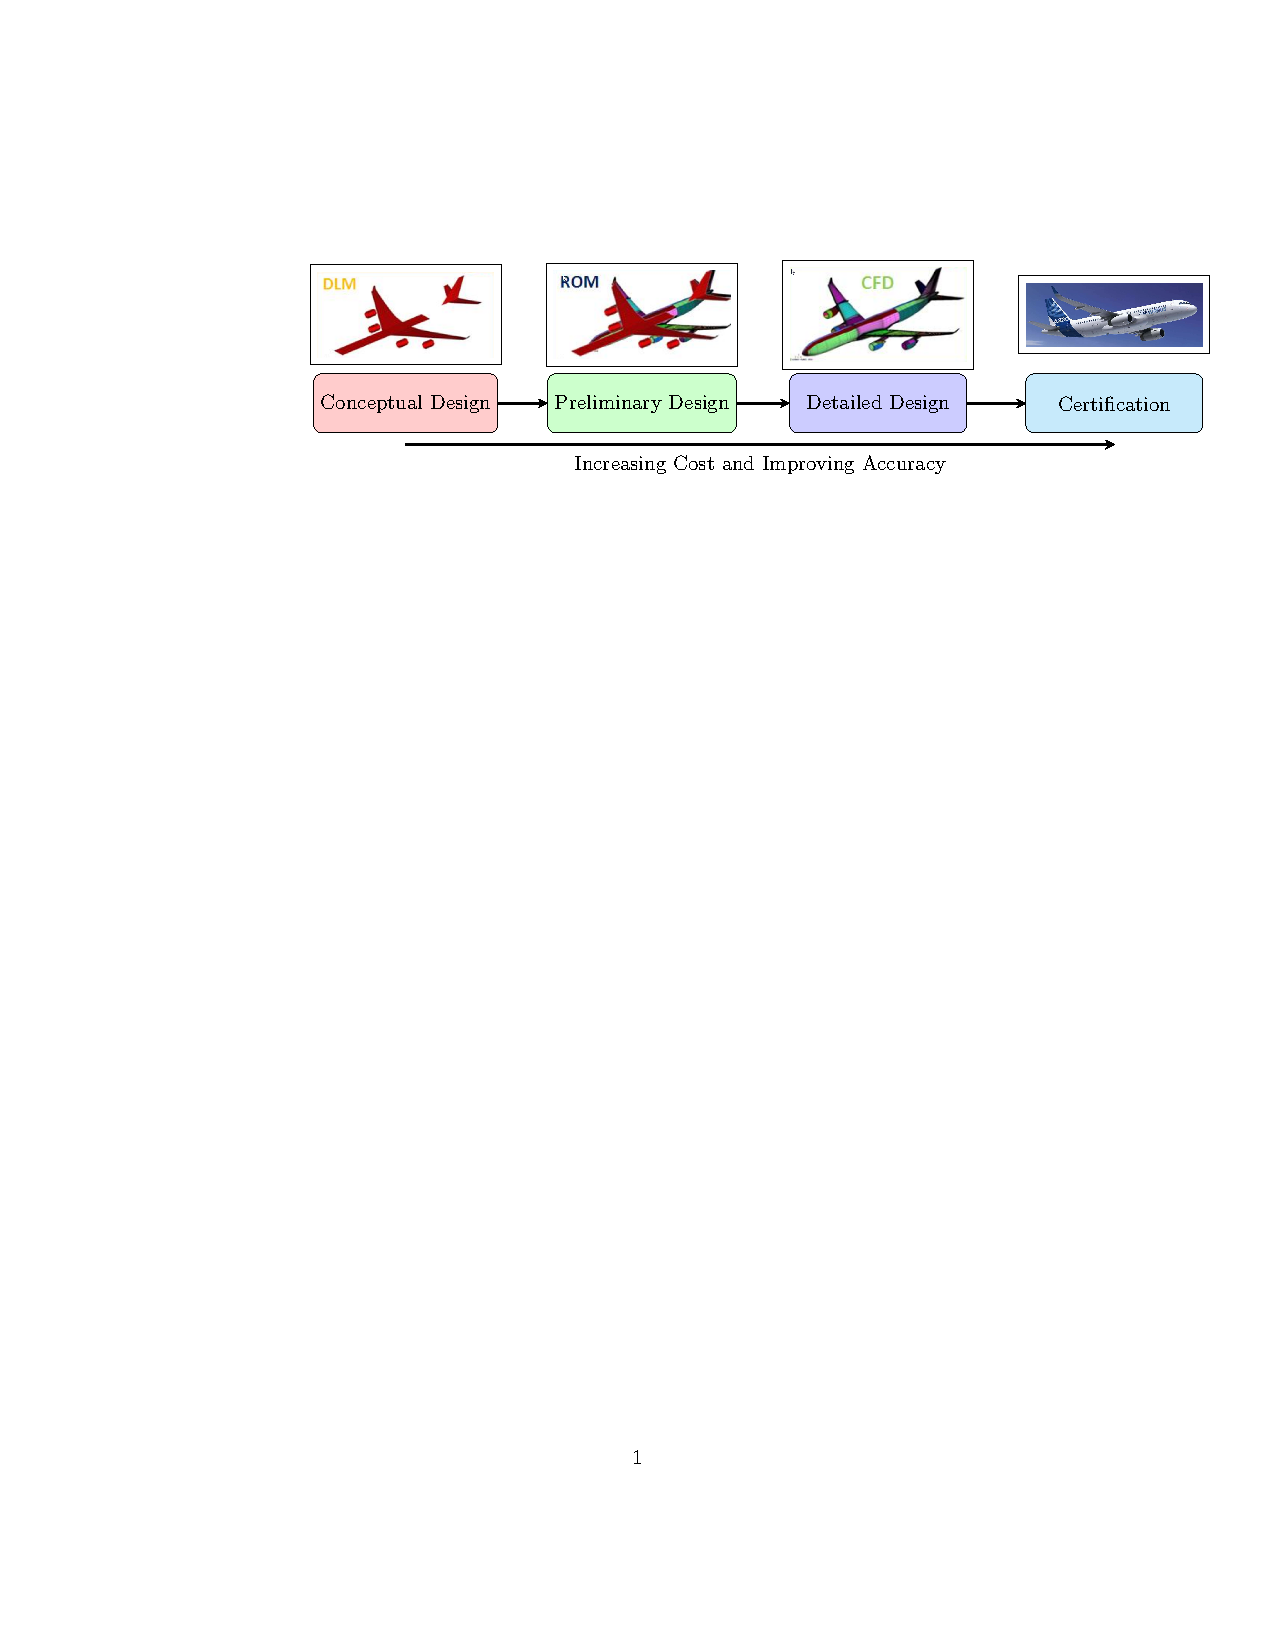
\includegraphics[clip, trim=4.5cm 19cm 0.5cm 4cm,width=0.95\textwidth]
    {flowchart/aircraftDesignCycleFlowChart}
  
  \caption{Phases of an aircraft design cycle}
\end{figure}

\section{Aircraft design cycle}\label{secSircraftDesignCycle}
\marginnote{\textsl{Design phases}}[1cm]
To simplify this process an aircraft design is broken down into several design phases (figure \ref{figPhasesOfAircraftDesign}). Each phase requires an ever increasing amount of predictions and fidelity. Preliminary design phase requires a few low-fidelity design trade-offs between major disciplines. Whereas, during detailed design phase, intensive intra-disciplinary and inter-disciplinary optimization's take place. Finally, during the flight-test and certification phase capability to predict real-time can provide significant gains in reducing the flight-test phase. These analyses cover large parts of flight envelope and require high-fidelity predictions. Hence the capability to accurately and quickly predict is an integral part of an aircraft design cycle \cite{raymer2012aircraft}. 

\marginnote{\textsl{Need for Speed}}[1cm]
In the last decade high-fidelity, physics based, non-linear mathematical simulations have become central to designing an aircraft. However, high-fidelity simulations are computationally expensive, this is the case for several Computational Fluid Dynamics (CFD) and Finite Element Method (FEM) based solvers. Due to this high cost high-fidelity simulations are launched only for a few carefully chosen configurations. This results in inefficient exploration of the the design space and thus a non-optimal design. A common strategy to speed up simulations is by reducing the physical complexity of the model to make quick predictions. As an example linear potential flows (simpler aerodynamic model), or coarser FEM meshes (simpler structural model) are regularly used during the preliminary design phase \cite{cummings2015applied}. While this is an acceptable practice during the preliminary design phase, during the detailed design phase physical complexity is needed to find a robust optimum design point \cite{raymer2012aircraft}.

\marginnote{\textsl{Need for accuracy}}[1cm]
Instead of approximating physical complexity, surrogate models\footnote{Surrogate models, learning algorithms and machine learning models will be used interchangeably throughout this manuscript} simplify mathematical complexity \cite{verveld2016reduced}. Surrogate models learn patterns between the input and output dataset and then are used to make predictions on the desired point. This property is very useful in quickly exploring the design space and finding a robust design point \cite{forrester2008engineering}. Moreover, surrogate models are commonly passed across disciplines to perform inter-disciplinary optimizations. For example, a loads department would prefer running a quick surrogate model over the costly CFD model while performing the load's loop.  

\marginnote{\textsl{Deduction vs Induction}}[1cm]
The main difference between the engineering design and surrogate modeling can be explained by the difference between deduction and induction \cite{domingos2012few} (figure \ref{fig:engineeringDesignVsSurrogateModelling}). Engineering design is deduction: where a very general formula is applied to a particular case (figure \ref{figDeduction}). The basics of Newtonian physics, when applied to a particular aircraft geometry, give inertial loads. The basics of aerodynamics, when applied to a particular set of aircraft geometry and aircraft states, give out aerodynamic pressures. Engineering design takes global rules and applies them to local configurations. Whereas, surrogate modeling is induction: it looks at local features and data, tries to find similarity measures between them and gives a global formula for the process (figure \ref{figInduction}). For example, an algorithm to detect faces in images will look at several images with and without faces, learn a facial pattern and make predictions on new images \cite{marszalek2007semantic}. We here see a possible complementary relationship between engineering design and machine learning; where engineering design needs models to generate data, machine learning needs data to generate models.

\begin{figure}[!ht]\label{fig:engineeringDesignVsSurrogateModelling}
  \centering
  \subfigure[Engineering design - Deduction: The figure shows an application of a general rule to a particular case.]
  {
    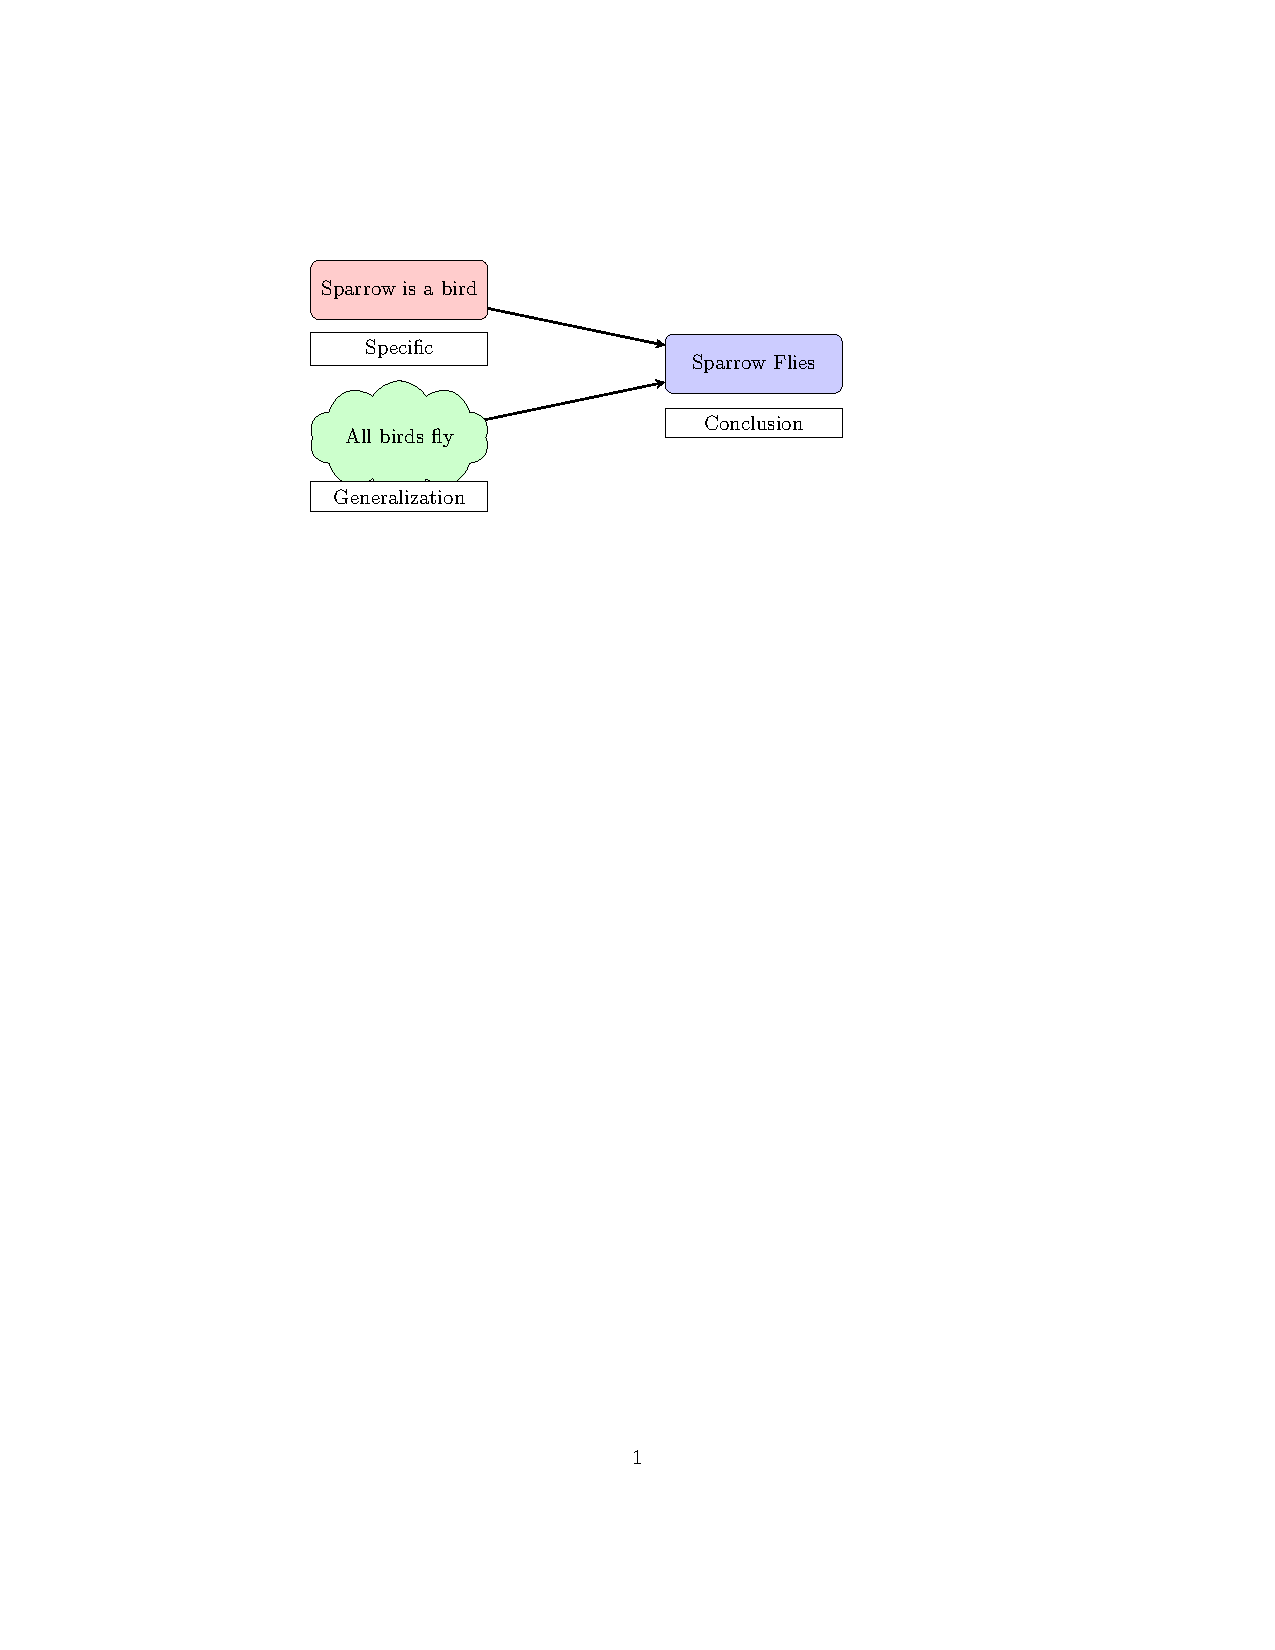
\includegraphics[clip, trim=4.5cm 19cm 4.5cm 4cm,width=0.45\textwidth]
    {flowchart/deduction}
    \label{figDeduction}
  }\quad
  \subfigure[Surrogate modelling - Induction: The figure shows how multiple examples can be used to infer underlying rules or patterns that govern the system.]
  {
    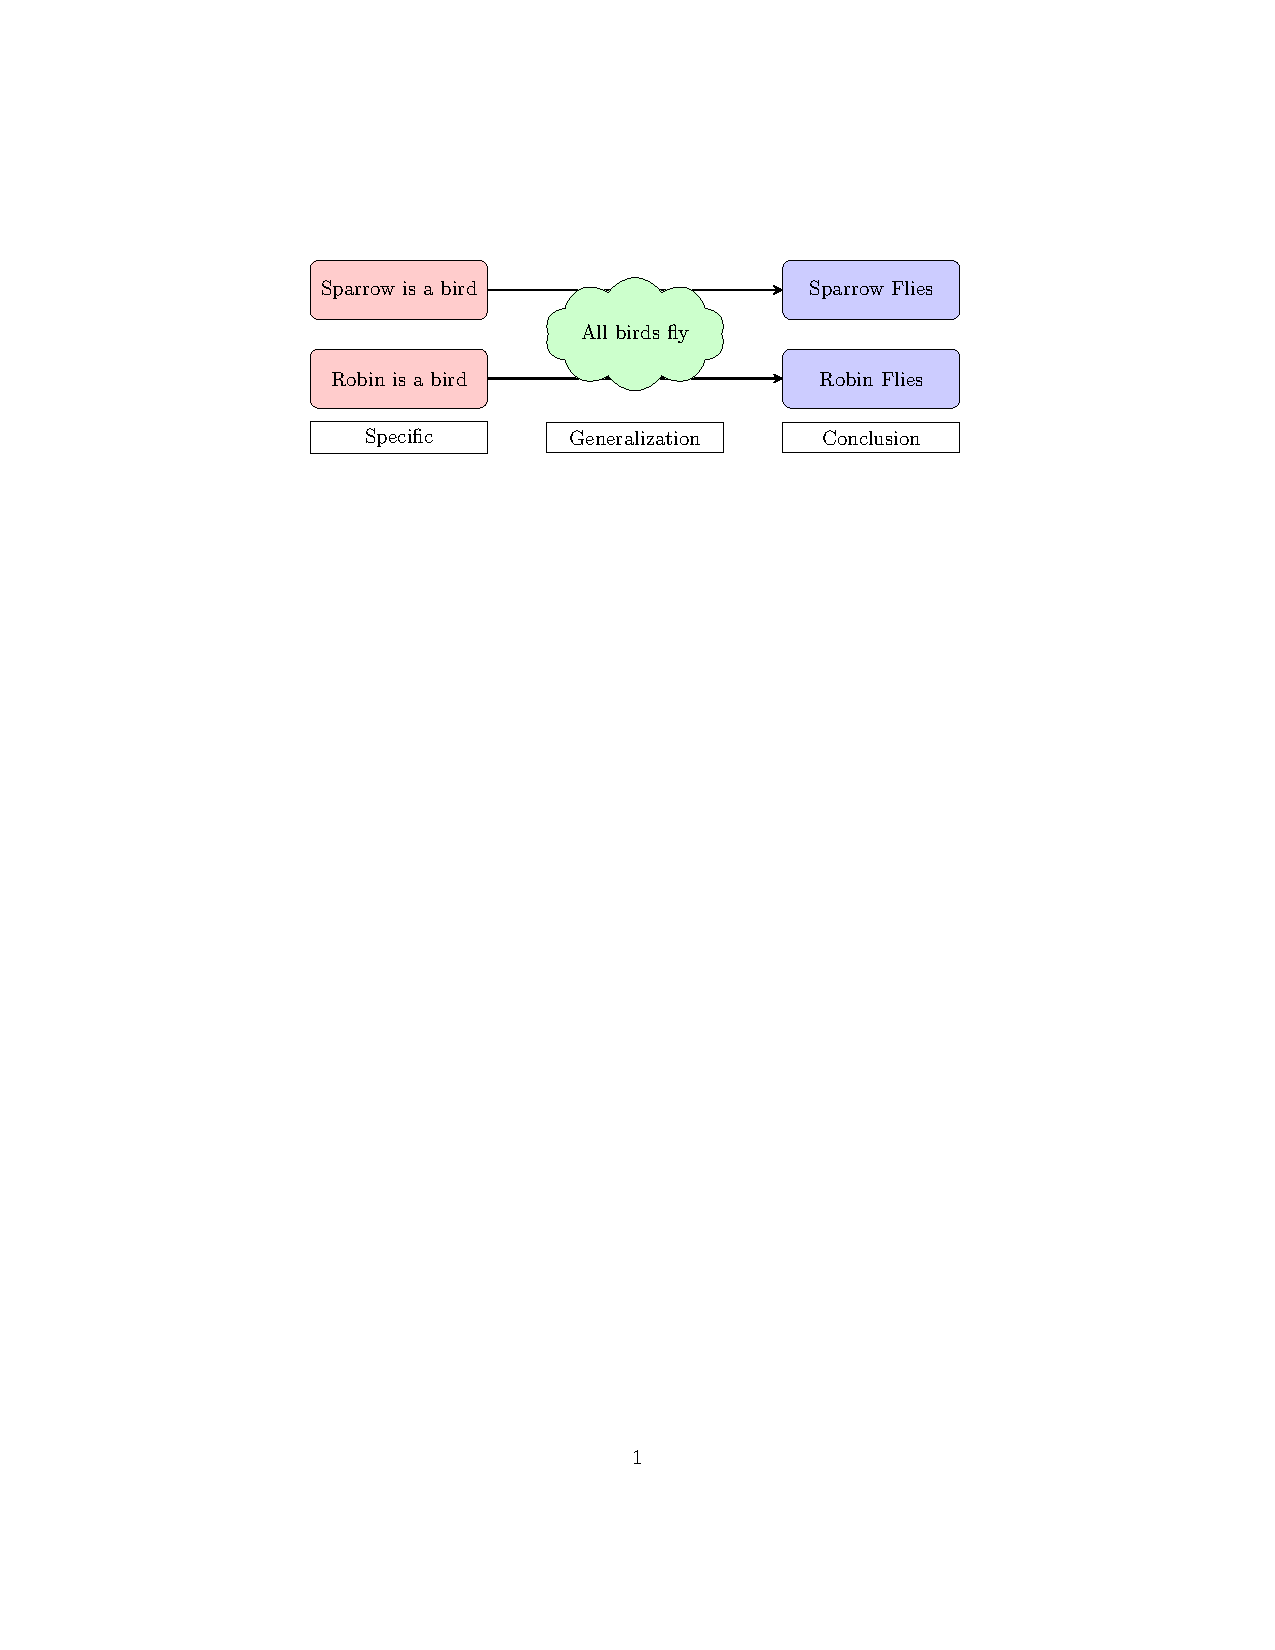
\includegraphics[clip, trim=4.5cm 20cm 4.5cm 4cm,width=0.45\textwidth]
    {flowchart/induction}
    \label{figInduction}
  }\quad
  \caption{Induction vs Deduction}
\end{figure}

\marginnote{\textsl{Developing faster models}}[1cm]
Since models are an integral part of any engineering design, model building in aircraft engineering was traditionally outsourced to research institutes. Researchers perform iterative experiments in a controlled environment and discover patterns between the physics of the system. For example, it took 200 years to iteratively develop the Gas law \footnote{\(Pressure \times Volume \approx numberOfMoles \times Temperature\)}, Boyle's law in 1600's found the relation between Pressure and Volume, Charle's Law in 1787 discovered the relationship between Volume and Temperature, while Gay-Lussac's Law in 1809 discovered the relationship between Pressure and Temperature \cite{clapeyron1834mémoire}. This is a rigorous and time-consuming method of developing models. Machine learning is a much more elegant method of building models. Using data and few basic assumptions, automatic models can be built between desired inputs and outputs. For example, while the first model of a neural network was proposed in 1950's \cite{kleene1951representation}, neural networks are today used daily for tasks such as tagging cat photos on facebook and converting speech to text\footnote{I wrote a fourth of this thesis using a text to speech software}. In this thesis, we wish to automatically build models for aircraft design tasks primarily to be used during the detailed design phase and certification phase. 


\section{Machine Learning}\label{secMachineLearning}
\marginnote{\textsl{Components of learning}}[1cm]
The core objective of learning algorithms is to find a transformation function between the inputs and outputs. There are three main components in a learning algorithm:
\begin{enumerate}
\item \textbf{Representation}: A learning algorithm starts with a family of functions. For example, a linear model is a family of linear functions, a trigonometric model defines a family of trigonometric functions. If an algorithm is not able to represent the actual function in its family of functions, it will find the closest function in its hypothesis space\footnote{The term family of functions, hypothesis space and representation will be used interchangeably throughout this manuscript}.
\item \textbf{Evaluation}: Some measure is needed to distinguish a good function from a bad function in the chosen hypothesis space. This measure is termed as evaluation; one example is the least squares error commonly used in many learning algorithms. 
\item \textbf{Optimization}: Finally, the algorithm iteratively searches in its hypothesis space to find the best possible function explaining the data. The choice of optimizer defines the speed of learning and is also important if there are multiple minima in the evaluation criteria.
\end{enumerate}

\marginnote{\textsl{Bias vs Variance}}[1cm]
Surrogate models suffer from the famous bias vs variance trade-off (figure \ref{figBiasVsVariance}), formalized by `Wolpert' in his famous "no free lunch theorem" \cite{wolpert1997no}. The constituent functions in a hypothesis space represent the bias or assumptions of the learning algorithm (eg. linear functions for linear regression). In the absence of sufficient assumptions, the family of functions in the search space becomes very large which leads to high variance or over-fitting in the surrogate model (figure \ref{subFigpredictionPoly15}). On the contrary, wrong bias means that the desired transformation function does not exist in the hypothesis space. In this case, the learning algorithm finds the closest function in its hypothesis space and leads to under-fitting (figure \ref{subFigpredictionPoly6}).

\begin{figure}[!ht]
  \centering
    \subfigure[{High-bias and low variance}]
  {
        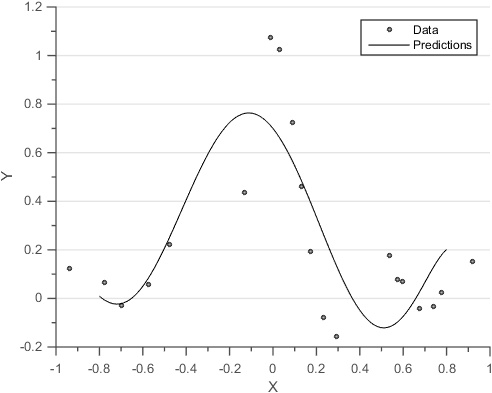
\includegraphics[width=0.29\textwidth]
        {images/predictionPoly6}
        \label{subFigpredictionPoly6}
  }\quad
\subfigure[{Low bias and High variance}]
  {
        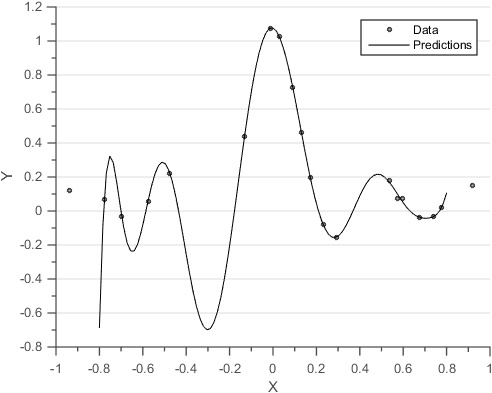
\includegraphics[width=0.29\textwidth]
        {images/predictionPoly15}
        \label{subFigpredictionPoly15}
  }\quad
  \subfigure[{Bias replaced with lots of data}]
  {
        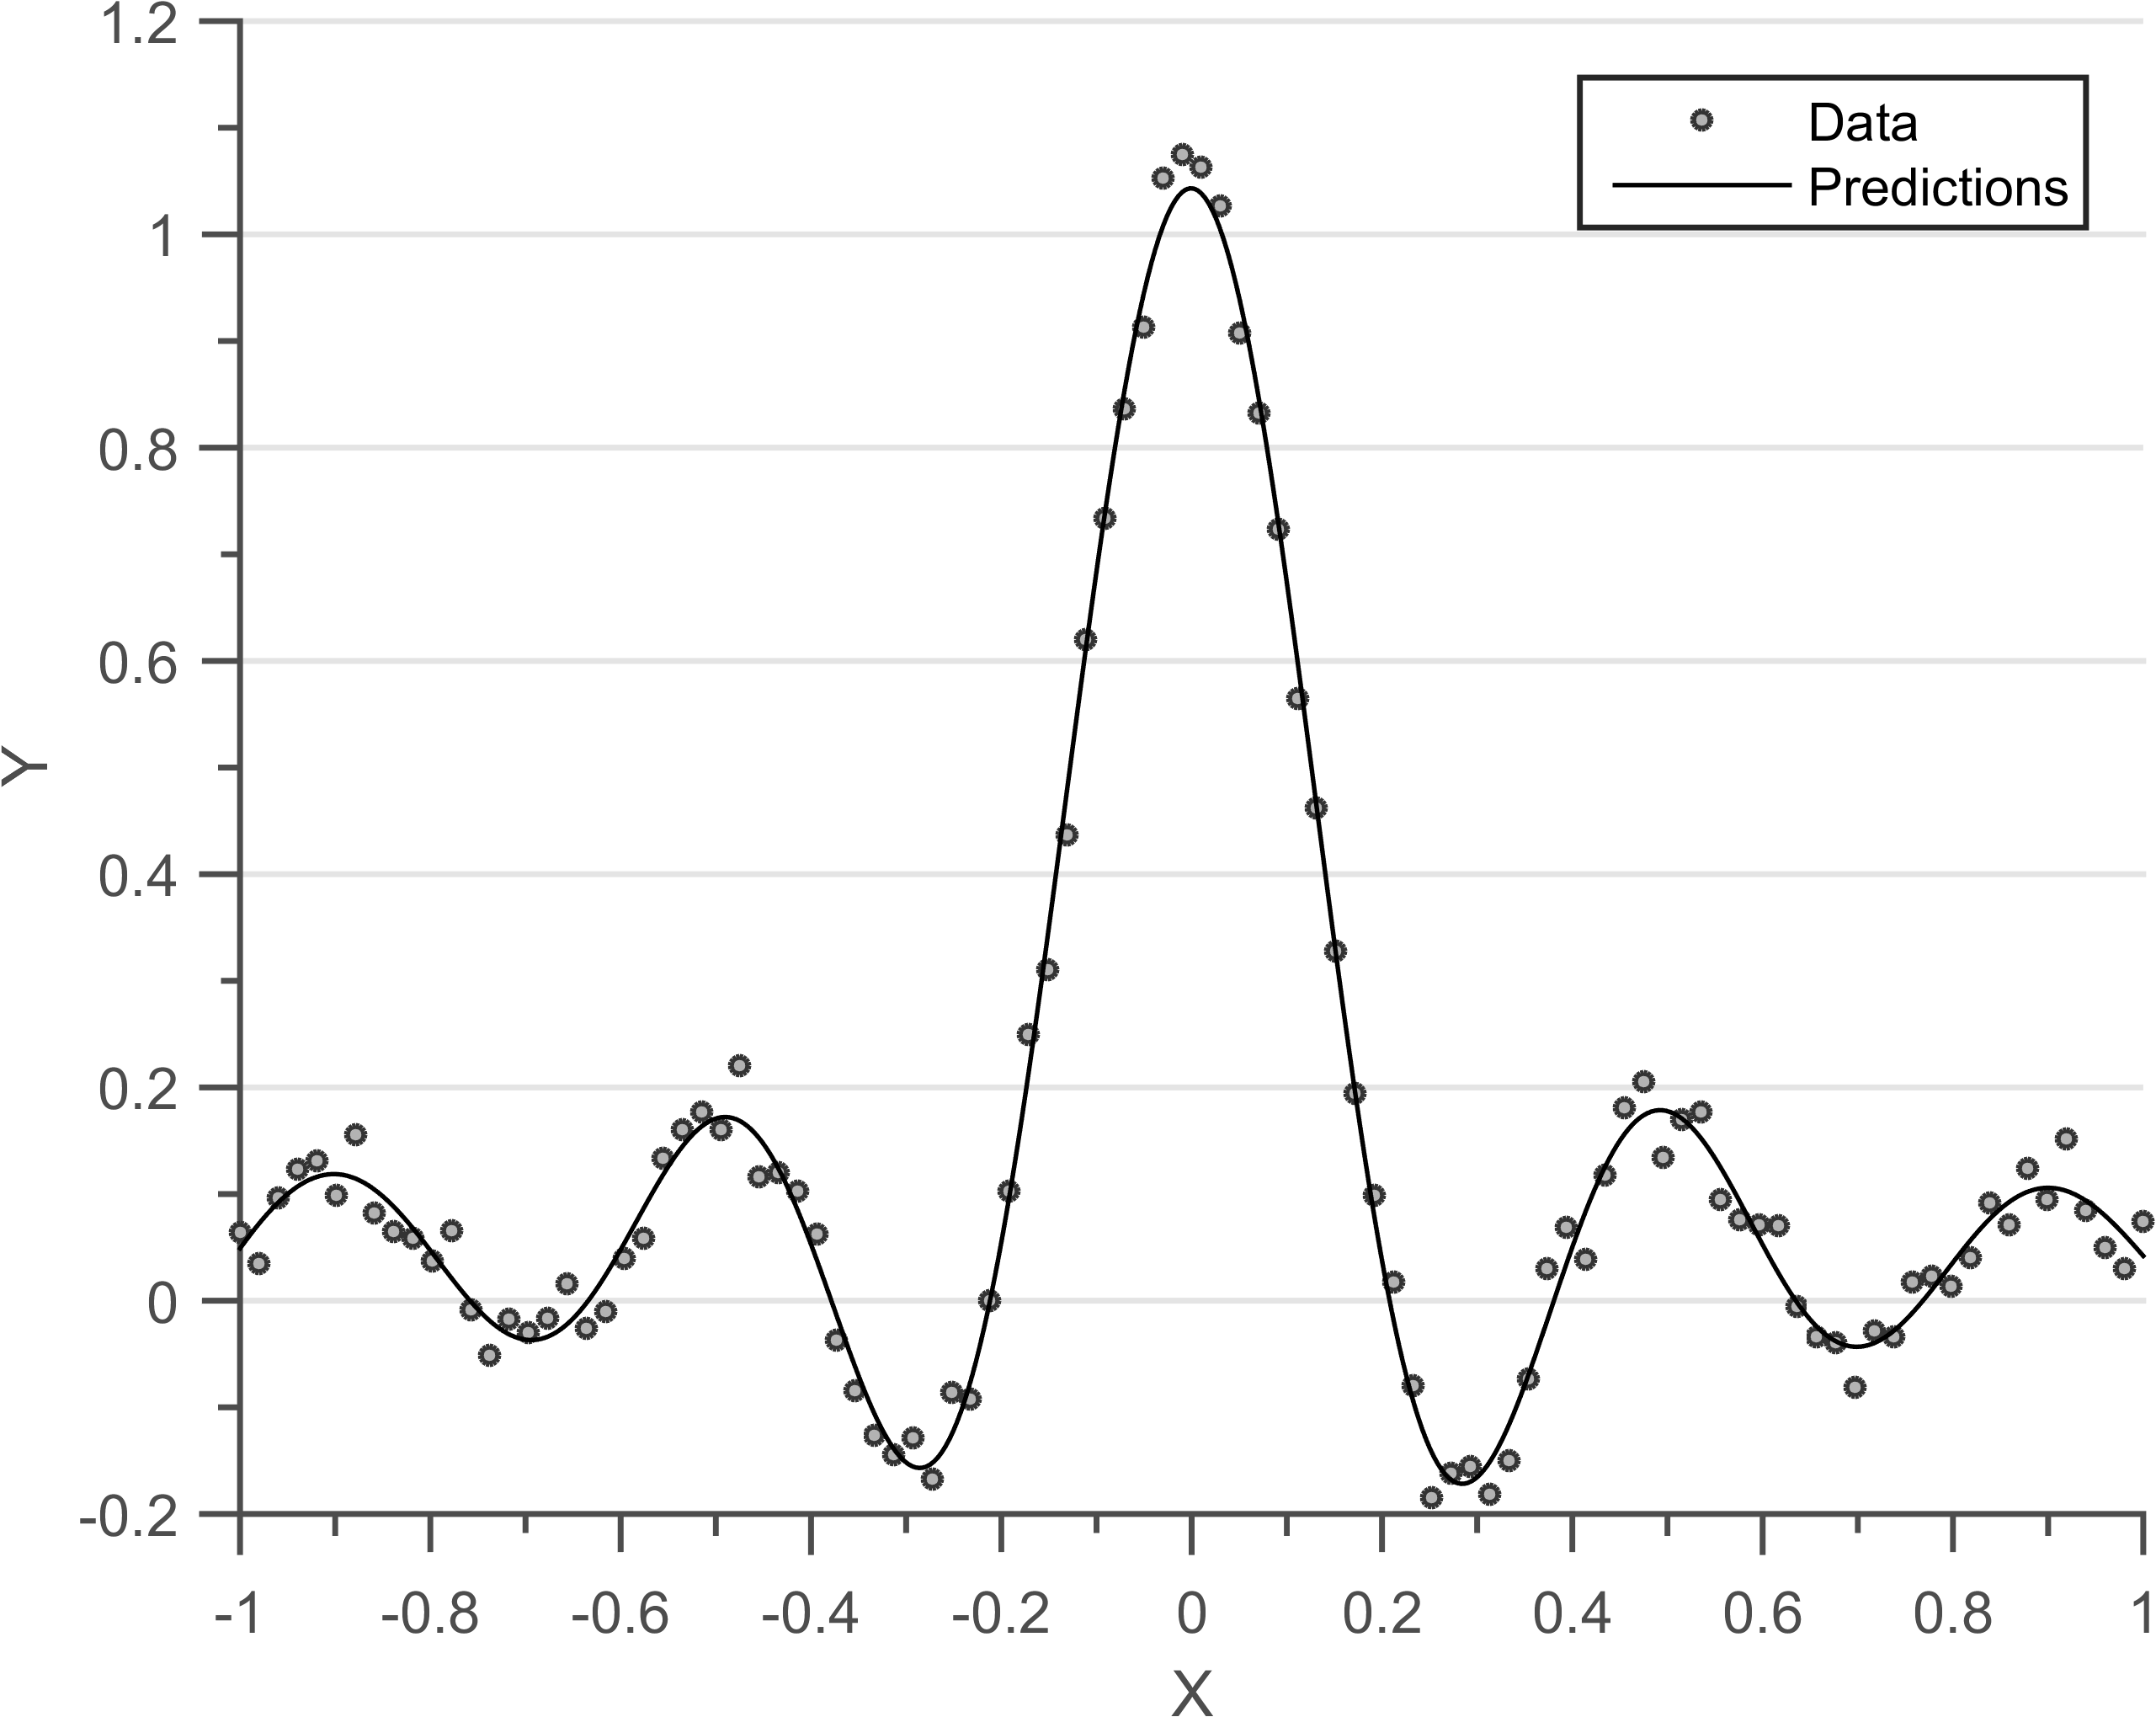
\includegraphics[width=0.29\textwidth]
        {images/posteriorSEInitialAtI100}
        \label{subFigposteriorSEInitialAtI100}
  }\quad
       \caption{Bias vs Variance trade-off}
       \label{figBiasVsVariance}
\end{figure}



\marginnote{\textsl{Soft and hard constraints}}[1cm]
One method to overcome this trade-off is by using lots and lots of data. Data acts as a hard constraint for learning algorithm, imagine a family of all possible continuous 2-dimensional functions in the range of $x \in [-1, 1]$ and $y \in [-1, 1]$. What will happen, given an observation $(x = 0, y = 0)$. All the functions that do not pass through this point will be eliminated, the new data point has basically reduced the possible family of functions. Whereas, bias acts as soft constraint, we can use the bias of linearity or smoothness to reduce our hypothesis space. Therefore, both bias and data help in reducing the hypothesis space\footnote{Bias can also be looked upon as distilled knowledge or patterns gained after interpreting huge amounts data}. Given access to more and more data we can progressively reduce the bias while learning models thereby relying more on true evidence. This is also the main concept behind deep learning, several layers of neural networks define a very large hypothesis space \cite{Goodfellow-et-al-2016, lecun2015deep}. 

Unfortunately, generating a huge amount of accurate data is a costly exercise in aircraft design e.g. a high fidelity CFD simulation runs for weeks \cite{murthy2014computational, jameson2012computational} and a flight-test campaign costs millions of euros \cite{fox2004test}. On another hand, we have a treasure trove of prior information about the physical systems, due to centuries of research and tinkering. We propose to build better machine learning models by integrating the time-tested available knowledge of physical systems with experimental data. 

\marginnote{\textsl{Contribution}}[1cm]
The main contribution of this thesis is to provide a framework on how to combine the prior knowledge from a physical system and add it to a learning algorithm. A model generated from merging of the two methodologies will be both consistent with the physics of the system and be quicker to evaluate. We integrate three types of prior knowledge by answering the following questions:
\begin{enumerate}
\item \textbf{Pattern}: How to add apriori information of a pattern in a learning algorithm? For example, given that shock is a discontinuous change in pressure, how to predict the position of shock on an airfoil (chapter \ref{chapStructureWithCovariance}). 
\item \textbf{Relationships}: How to add apriori information of relationships between measurements? For example given \(Loads = \int Pressures\), how to make a robust loads model when we measure both pressures and loads (chapter \ref{chapAddingEquationsInGP}).
\item \textbf{Simulation model}: How to merge apriori information of simulations with experiments? For example, given a simulation model and experimental data how to perform extrapolations on experimental data(chapter \ref{chapMultiTaskExtrapolation}). 
\end{enumerate}

To integrate the prior information we propose to use a Bayesian inference for model building. Bayesian inference is a method of statistical inference in which Bayes theorem is used to update an initial probability (prior) as more and evidence becomes available the final probability (posterior) gives our estimate. More specifically, we will use the Gaussian Processes (GP) Regression framework which is a subset of the Bayesian Inference algorithms to define prior information of physical systems. But, before deep diving into the details of GP let us have a look at a simple Bayesian Linear Regression algorithm.

\section{Bayesian Linear Regression}\label{secBayesianModelling}
Suppose we have access to a training set of observations (or outputs) \(Y = (y(x_{1}); \ldots ; y(x_{i}); \ldots ; y(x_{N}))\), evaluated at a set of known inputs \(X = (x_{1}; \ldots ; x_{i}; \ldots; x_{N})\), and we wish to predict \(y(x_{*})\) at a test input \(x_{*}\). The input and output can be multi-dimensional; \(x_{i} \in \mathbb{R}^{D_{inputs}}\) and \(y(x_{i}) \in \mathbb{R}^{D_{outputs}}\). The process of learning the transformation function \(f\) to make prediction at a new point is called as regression. In the following section we follow formulation for Bayesian Linear Regression provided by \cite{mackay2003information}.

\marginnote{\textsl{Basis functions}}[1cm]
A simple method to perform regression is by assuming a parametrized form of the function \(f\) and then minimizing the error between measurements and predictions to estimate the parameters of function. The function is written in terms of basis functions \(\phi(x)\). For example when \(\phi(x) = \{1, x\}\) we are performing linear regression, when \(\phi(x) = \{1, x, x^{2}, \ldots, x^{L}\}\) we are performing \(L^{th}\) order polynomial regression. We will focus on linear regression in this section and hence \(\phi(x) = \{1, x\}\).

\begin{equation}\label{eqBayesianLinearRegression}
f(x_{i}) = \begin{Bmatrix}
x^{0} & x^{1}
\end{Bmatrix}  \begin{Bmatrix}
w_{0}\\ 
w_{1}
\end{Bmatrix}
\quad \quad y(x_{i}) = f(x_{i}) + \epsilon
\end{equation}

\marginnote{\textsl{Likelihood}}[1cm]
Here, \(w\) are the parameters of the function. The measurements are corrupted by independent white noise \(\epsilon\), such that the noise is a random variable sampled from a white noise Gaussian with variance \(\sigma_{n}^{2}\)\footnote{\(\Pr[\epsilon] = \mathcal{N}(0, \sigma_{n} = \frac{1}{\sqrt{2\pi\sigma_{n}^{2}}}\exp^{-\frac{\epsilonç{2}}{2\sigma_{n}^{2}}}
)\)}. The above equations \ref{eqBayesianLinearRegression} can be combined to result in the likelihood \(\Pr[Y\mid X, w]\)

\begin{equation}\label{eqBayesianLikelihood}
\begin{aligned}
\Pr[Y \mid X, w]  & = \prod \Pr[y_{i}\mid x_{i}, w]\\
                & = \prod \mathcal{N}[x_{i}w , \sigma_{n}^{2}]\\
                & = \mathcal{N}(X w, \sigma_{n}^{2}I)    
\end{aligned}
\end{equation}

The notation \(\Pr[Y \mid X, w]\) symbolizes probability distribution of observations \(Y\) at the inputs \(X\) given the parameter \(w\). The notation \(\mathcal{N}[\mu , \Sigma]\) symbolizes a multi-variate Gaussian distribution for mean vector \(\mu\) and covariance matrix \(\Sigma\). 

\marginnote{\textsl{Prior}}[1cm]
While performing Bayesian inference we specify a prior distribution to encode our assumptions on the parameters before we look at the observations. For this case, we put a zero mean Gaussian prior on our weights.

\begin{equation}\label{eqBayesianPrior}
\Pr[w] = \mathcal{N}(0, \Sigma_{Prior})
\end{equation}

The prior distribution on \(w\) induces a prior distribution over functions parametrized by \(w\), effectively we are defining family of functions \((\Pr[f(x_{i})] = \mathcal{N}(0, x_{i}^{T}\Sigma_{Prior}x_{i}))\) by placing a prior distribution over \(w\). Once we have a prior distribution encoding our beliefs, we use Bayes rule to look at the observations and get a posterior distribution of parameters.

\begin{equation*}
posterior = \frac{likelihood \times prior}{marginal \quad likelihood}
\end{equation*}
\begin{equation}\label{eqBayesRule}
\Pr[w \mid Y, X] = \frac{\Pr[Y \mid X, w] \times \Pr[w]}{\Pr[Y \mid X]}
\end{equation}

\marginnote{\textsl{Marginal Likelihood}}[1cm]
The \textsl{marginal likelihood} is a normalization constant, for more details please refer to section \ref{secHyperParameter}. After, using the equation \ref{eqBayesianLikelihood}, \ref{eqBayesianPrior} and \ref{eqBayesRule} we can get the posterior distribution of weights as:

\begin{equation}\label{eqBayesianPosterior}
\Pr[w \mid Y, X]  = \mathcal{N}\left ( \frac{1}{\sigma_{n}^{2}} A^{-1}X Y , A^{-1} \right )
\end{equation}

Here, \(A = \sigma_{n}^{-2}XX^{T} + \Sigma_{Prior}^{-2}\). Thus the posterior distribution for function \(f\) at test point \(x_{*}\) becomes:

\begin{equation}\label{eqBayesianFunctionalPosterior}
\Pr[f \mid x_{*}, X, y]  = \mathcal{N}\left ( \frac{1}{\sigma_{n}^{2}} x_{*}A^{-1}XY , x_{*}^{T}A^{-1}x_{*} \right )
\end{equation}

\marginnote{\textsl{Posterior}}[1cm]
The mean \(\frac{1}{\sigma_{n}^{2}} x_{*}A^{-1}XY\) can be used as a prediction at the test point \(x_{*}\), while the variance is a measure of uncertainty for this prediction. We can thus obtain the prediction \(f(x_{*})\), using a prior set of beliefs (equation \ref{eqBayesianPrior}) and updating those beliefs using observations. While the Bayesian Linear Regression framework provides an opportunity to encode prior assumptions in terms of distributions of the parameters. A much more elegant and expressive method is by using Gaussian Processes to perform regression. Gaussian Processes are a distribution over functions and hence enable us to encode prior knowledge directly in the functional space. 

\marginnote{\textsl{Non-parametric models}}[1cm]
Learning algorithms are mainly divided into two main types. The first is defined by parametric models which can only represent a limited hypothesis space. They use parameters to describe the function between input and output domain. For example the weight parameters \(w\) in Bayesian Linear Regression. The second are non-parametric models whose hypothesis space grows with the size of data. Non-parametric models use data to represent functions, Gaussian Process Regression is a type of non-parametric model. One can imagine a non-parametric model like a stretched rubber sheet: whenever it sees data it deforms accordingly to compensate for the new data point. Hence the more data it sees the more it starts mimicking the actual function. 

\marginnote{\textsl{Gaussian Process}}[1cm]
Gaussian Process or Kriging was first used in the context of Geo-statistics research by Daniel Krige \cite{krige1951statistical}, this was later formalized by Matheron in his seminal work "Principals of Geo-statistics" \cite{matheron1963principles}. Recently, interest in the Gaussian Process (GP) grew in the machine learning community from neural networks research. It was shown that a Bayesian neural network becomes a Gaussian process as the number of neurons tends to infinity \cite{neal2012bayesian}. Gaussian processes are probabilistic distributions over functions, which provide a Bayesian non-parametric approach to smoothing and interpolation. A Gaussian Process can be fully parameterized by its mean and covariance function. More generally, a Gaussian Process is a method to probabilistically define a family of functions, chapter \ref{chapGp} expands GP in more detail. 

\section{Outline}\label{secOutline}
This thesis is divided into three main parts, each part is then divided into individual chapters and their constituent sections. This part sets up the prerequisites required to understand the concepts introduced in the next two parts. The first chapter demonstrates the need for performing regression in aircraft design tasks and describes a very basic Bayesian Linear Regression scheme. 

\marginnote{\textsl{Chapter \ref{chapGp}}}[1cm]
Chapter \ref{chapGp} shows the key processes involved in a GP regression framework. GPs as distributions over functions have a rich history in geo-statistics and machine learning. The second chapter heavily draws ideas from \cite{krige2015statistical, matheron1963principles} of the geo-statistics community and \cite{Stein1999Springer, kennedy2000predicting, Rasmussen2005, mackay2003information} of the machine-learning community, showing a process flow of how to perform regression using GPs. The remaining chapter unfolds as follows, section \ref{secPrior} describes the key constituents of a GP and how to draw random functions from a GP. Section \ref{secPosterior} describes how to perform prediction in presence and absence of measurement noise. Section \ref{secHyperParameter} introduces marginal likelihood as a form of evaluation method to automatically choose hyper-parameters. 

\marginnote{\textsl{Chapter \ref{chapSparseGPRegression}}}[1cm]
Chapter \ref{chapSparseGPRegression} deals with the problem of scaling GP regression to massively many points. Traditional GPs are computationally infeasible on a standard laptop if the number of data points increase \(\mathcal{O}(10^4)\). There exist two main methods to scale a GP regression, one using reduced set of inducing points while another based on mixture of experts methodology. This chapter draws heavily from the works of \cite{quinonero2005unifying, seeger2003fast, Snelson06sparsegaussian, Titsias09variationallearning} for the approximation method of inducing points and \cite{cao2014generalized, tresp2000bayesian, chen2009bagging, deisenroth2015distributed} for the approximation method of mixture of experts, please refer to the individual publications for more detail. We demonstrate the limitations and capabilities of both the methods on a toy dataset, giving directions to choosing optimal parameters and extracting the best possible result.  

\textbf{Description of the other two parts}

%%% Local Variables: 
%%% mode: latex
%%% TeX-master: "isae-report-template"
%%% End: 

\chapter{Gaussian Process Regression}
\label{chapGp}

Suppose we perform a simulation or experiment on an input point $x_{j} \in \mathbb{R}^{D_{inputs}}$and measure an output $y_{j} \in \mathbb{R}$. In this chapter we assume that the input is $D_{inputs}$ dimensional and the output is one dimensional. We can thus have a data set of $N$ observations, $\{\mathcal{D} = (x_{j}, y_{j}) | j \in [1; N] \}$. The full input and output vectors can be denoted as $X = \{x_{1}; x_{2}; \ldots ; x_{N}\}$ and $Y = \{y_{1}; y_{2}; \ldots ; y_{N}\}$ such that $X \in \mathbb{R}^{N \times P}$ and $Y \in \mathbb{R}^{N }$. Given this data we are interested in making predictions for new input points $x_{*}$ \footnote{Also called as test point, prediction point or target point.}that are not present in our series of experiments. This means that we need to use out training data and learn, the true physical process  $f(x)$ that generates our data set.

As discussed in the previous chapter, to learn the governing function $f(x)$ we first start with a family of functions. Gaussian Process (GP) can be used to probabilistically define a family of functions. More formally, a GP is a distribution over functions such that any finite set of function values $[f(x_{1}), f(x_{2}), \ldots, f(x_{N})]$ have a joint Gaussian distribution \cite{rasmussen2006gaussian}. 

\marginnote{\textsl{Infinite dimensional random vector}}[1cm]
While a normal distribution describes a scalar random variable, example $X \sim \mathcal{N}(0, 1)$ defines a Gaussian variable with mean $0$ and variance $1$. A multi variate distribution defines a vector of random variables, for example $\{X\} \sim \mathcal{N}(\{0, 0\}, [1, 0; 0, 1])$ defines a Gaussian vector with mean $\{0, 0\}$ and covariance $[1, 0; 0, 1]$. A GP is the extension of this concept in the functional space. We can also think of a function as an infinite dimensional vector, each entry in the vector specifying the function value $f(x)$ at a particular point $x$ \footnote{Yes blew my mind as well!}. 

\marginnote{\textsl{Mean}}[1cm]
A GP model before conditioning on data can be completely parameterized by its mean

\begin{equation}\label{eq:meanGP}
\mathbf{E}[f(x)] = m(x)
\end{equation}

\marginnote{\textsl{Covariance}}[1cm]
and its covariance function also called a kernel. In the context of the GPs a kernel is a measure of similarity between pairs of functional values $(f(x))$ evaluated at input points , often involving an inner product of basis functions $\phi(x)$ \cite{bishop2006pattern}. Please refer to chapter \ref{chapBasicCovarianceKernels} for a more detailed insight into kernels.   \footnote{The terms covariance functions, kernel and kernel functions will be used interchangeably during the reminder of this thesis}:

\begin{equation}\label{eq:covarianceGP}
Cov[f(x) - m(x), f(x') - m(x')] = k(x_{1}, x_{2})
\end{equation}

We can formally write the probability of the function $f$ as:

\begin{equation}\label{equationGPdefinition}
\Pr[f(x)] = GP(m(x), k(x_{1}, x_{2}))
\end{equation}

The notation $\Pr(f( x))$ symbolizes probability distribution of function $f$ at the inputs $x$. A function randomly drawn from a GP yields a random function around the mean function $m(x)$ and of the shape as defined by covariance function $k(x_{1}, x_{2})$. 

\marginnote{\textsl{Tractable}}[1cm]
Performing inference on an infinite dimensional vector (function) can be a computationally intensive task. Thankfully, due to the marginalization property of Gaussians, if we ask for properties of the function at a finite number of points, then  GP will give us the same answer if we ignore the infinitely many other points. In other words any finite set of function values $[f(x_{1}), f(x_{2}), \ldots, f(x_{N})]$ have a joint Gaussian distribution in GP (also the  definition of GP). This property means that GP specified in equation \ref{equationGPdefinition} also specifies equation \ref{equationGPMarginalizationProperty}. This makes GPes computationally tractable, one of the major benefits of GP. 


\begin{equation}\label{equationGPMarginalizationProperty}
\Pr\left [ \begin{matrix}
f(x_{1})
\\ f(x_{2})
\end{matrix} \right ] = \mathcal{N}\left (\left [ \begin{matrix}
m(x_{1})
\\ m(x_{2})

\end{matrix} \right ] , \left [ \begin{matrix}
k(x_{1}, x_{1}) & k(x_{1}, x_{2})\\ 
k(x_{2}, x_{1}) & k(x_{2}, x_{2})
\end{matrix} \right ] \right )
\end{equation}

While performing regression in a GP framework we first define a family of functions also called prior (section \ref{secPrior}). The next step involves taking observations and eliminating all the functions in our prior which do not obey the observations, this step gives us the posterior mean and variance (section \ref{secPosterior}). Finally, we can further improve our predictions by fine-tuning our hyper-parameters (section \ref{secHyperParameter}).

\section{Prior} \label{secPrior}
In the Bayesian framework, a prior is a probability distribution before looking at any evidence. In the context of a GP Regression, this is provided by the mean and covariance function. 

\subsection{Hyperparameters}
Both mean and covariance functions are specified by a set of hyper-parameters $\theta$. The hyper-parameters are very similar to weight parameter ($w$) during Bayesian Linear Regression (section \ref{secBayesianModelling}), these are the parameters of the GP. Selecting a prior in GP boils down to choosing an appropriate functional form of the mean and covariance matrix and then choosing the hyper-parameters of the prior \cite{duvenaud2013structure}. 

Automatically, predicting the values of hyper-parameters is important to choose a good prior. We will look at how to choose good hyper-parameters in section \ref{secHyperParameter}. 

\subsection{Mean function}\label{subSecCH2MeanFunction}
The mean function $m(x)$ of a GP represents its trend. In Universal Kriging, we usually choose a mean function of the form $m(x) = \phi(x)^{T}\theta$, with $\phi(x) = (\phi_{1}(x), \ldots , f_{p}(x))$ being a vector of basis functions, generally including a constant function and $\theta \in \mathbb{R}^{p}$ is a vector of hyper-parameters \cite{matheron1963principles}. In Simple Kriging we assume a constant mean function $m(x) = \theta$.

\marginnote{\textsl{Zero mean}}[1cm]
Without loss of generality, we can assume the mean function to be zero everywhere, since uncertainty about the mean function can be taken into account by adding an extra term to the covariance function (Chapter \ref{chapBasicCovarianceKernels}).  

\begin{equation}\label{equationMeanZeroGPdefinition}
\Pr[f(x)] = GP(0 , k(x_{1}, x_{2}, \theta))
\end{equation}

We assume a zero mean prior through out this section. After accounting for the zero mean, the GP model can be completely parametrized by the kernel. Hence the problem of learning in a GP is exactly the problem of finding suitable properties of the covariance function \cite{rasmussen2006gaussian} (equation \ref{equationMeanZeroGPdefinition}). 


\subsection{Covariance function}\label{subSecCH2Covariance}
The covariance function is a positive definite kernel, such that for any $a_{i} \in \mathbb{R}$ equation \ref{equationPDKernel} holds \cite{Stein1999Springer}.

\begin{equation}\label{equationPDKernel}
\sum_{i=1}^{N}\sum_{j=1}^{N}a_{i}a_{j}k(x,x') \geq 0
\end{equation}

A popular choice of covariance function is a Squared Exponential (SE) function (equation \ref{eqnSquaredExponential}), because it defines a family of highly smooth (infinitely differentiable) non-linear functions as shown in figure \ref{figGPPriors}.

\begin{equation}\label{eqnSquaredExponential}
k_{SE}(x_{1}, x_{2}, \theta) = \theta_{amplitude}^2exp[-\frac{d^2}{2\theta_{lengthScale}^2}]
\end{equation}

\marginnote{\textsl{SE kernel}}[1cm]
For the case of the SE kernel the hyper-parameters $(\theta = [\theta_{amplitude}, \theta_{lengthScale}])$ are; amplitude $(\theta_{amplitude})$ which defines average distance from mean and the length scale $(\theta_{lengthScale})$ which defines the smoothness of functions. Here, $d$ defines the absolute distance between points $|x-x'|$. Covariance functions which are purely a function of distance $d$ are called as isotropic stationary functions. These covariance functions remains unchanged if the points $x_{1}, x_{2}$ are rotated or translated. Hence a family of functions defined by stationary kernels will have similar local features throughout the input domain. 

\marginnote{\textsl{Length-Scale}}[1cm]
When $x$ tends to $x'$ then $k(x_{1}, x_{2})$ approaches $\theta_{amplitude}^{2}$, this means that $f(x)$ is highly correlated with $f(x')$. This is a good characteristic for smooth functions, since points in the neighbourhood must be alike. If $x$ is far away from  $x'$ then $k(x_{1}, x_{2})$ tends to zero, this means that far away points are loosely correlated. Hence, far off observations will have negligible effect while performing interpolations. How fast or slow the covariance decreases with distance depends on the length scale parameter $\theta_{lengthScale}$, smaller length-scale means a faster moving function. In general we cannot extrapolate more than $\theta_{lengthScale}$ units from the closest data-point \cite{duvenaud-thesis-2014}. 

\subsection{Sampling functions from GP priors}\label{subSecSamplingFunctionsGPPrior}
To have a look at the constituent functions in a prior we can randomly sample functions from the GP. Since any finite set of set of function values have a joint Gaussian distribution in a GP. To draw random functions from a GP we choose $N*$ input points $X_{*} = \{x_{1*}; x_{2*}; \ldots ; x_{N*}\}$ and write corresponding mean vector $m(X_{*})$ and covariance matrix $K(X_{*}, X_{*} )$ \footnote{The covariance matrix is also called the Gram matrix} using equation \ref{equationGPMarginalizationProperty} and \ref{eqnSquaredExponential}. We then generate a random Gaussian vector $f(X_{*})$ for this multi-variate Gaussian (equation \ref{equationMeanZeroGPdefinition}) and plot the generated values as a function of inputs $X_{*}$. 

\begin{equation}\label{eqnCovMatrixSquaredExponential}
K(X_{*}, X_{*} ) = \left [ \begin{matrix}
k(x_{1*}, x_{1*}) & k(x_{1*}, x_{2*}) & \ldots & k(x_{1*}, x_{N*})
\\ k(x_{2*}, x_{1*}) & k(x_{2*}, x_{2*}) & \ldots & k(x_{2*}, x_{N*})
\\ \vdots & \vdots & \ddots & \vdots
\\ k(x_{N*}, x_{1*}) & k(x_{N*}, x_{2*}) & \ldots & k(x_{N*}, x_{N*})
\end{matrix} \right ] 
\end{equation}

Figure \ref{figGPCovarianceMatrix} shows the covariance matrix for Standard Exponential kernel with different hyper-parameters at the input points $X^{*} = \{[0:0.02:1]\}$. The SE kernel of figure \ref{subFigcovSEmatrix_1} has a lower length-scale than figure \ref{subFigcovSEmatrix_2}. Note, how the covariance values are more spread out for figure \ref{subFigcovSEmatrix_2}.

\begin{figure}[!ht]
  \centering
    \subfigure[{Covariance matrix for a Standard Exponential (SE) Kernel with $(\theta = [1, 0.2])$ at the input points $X^{*} = \{[0:0.02:1]\}$. }]
  {
        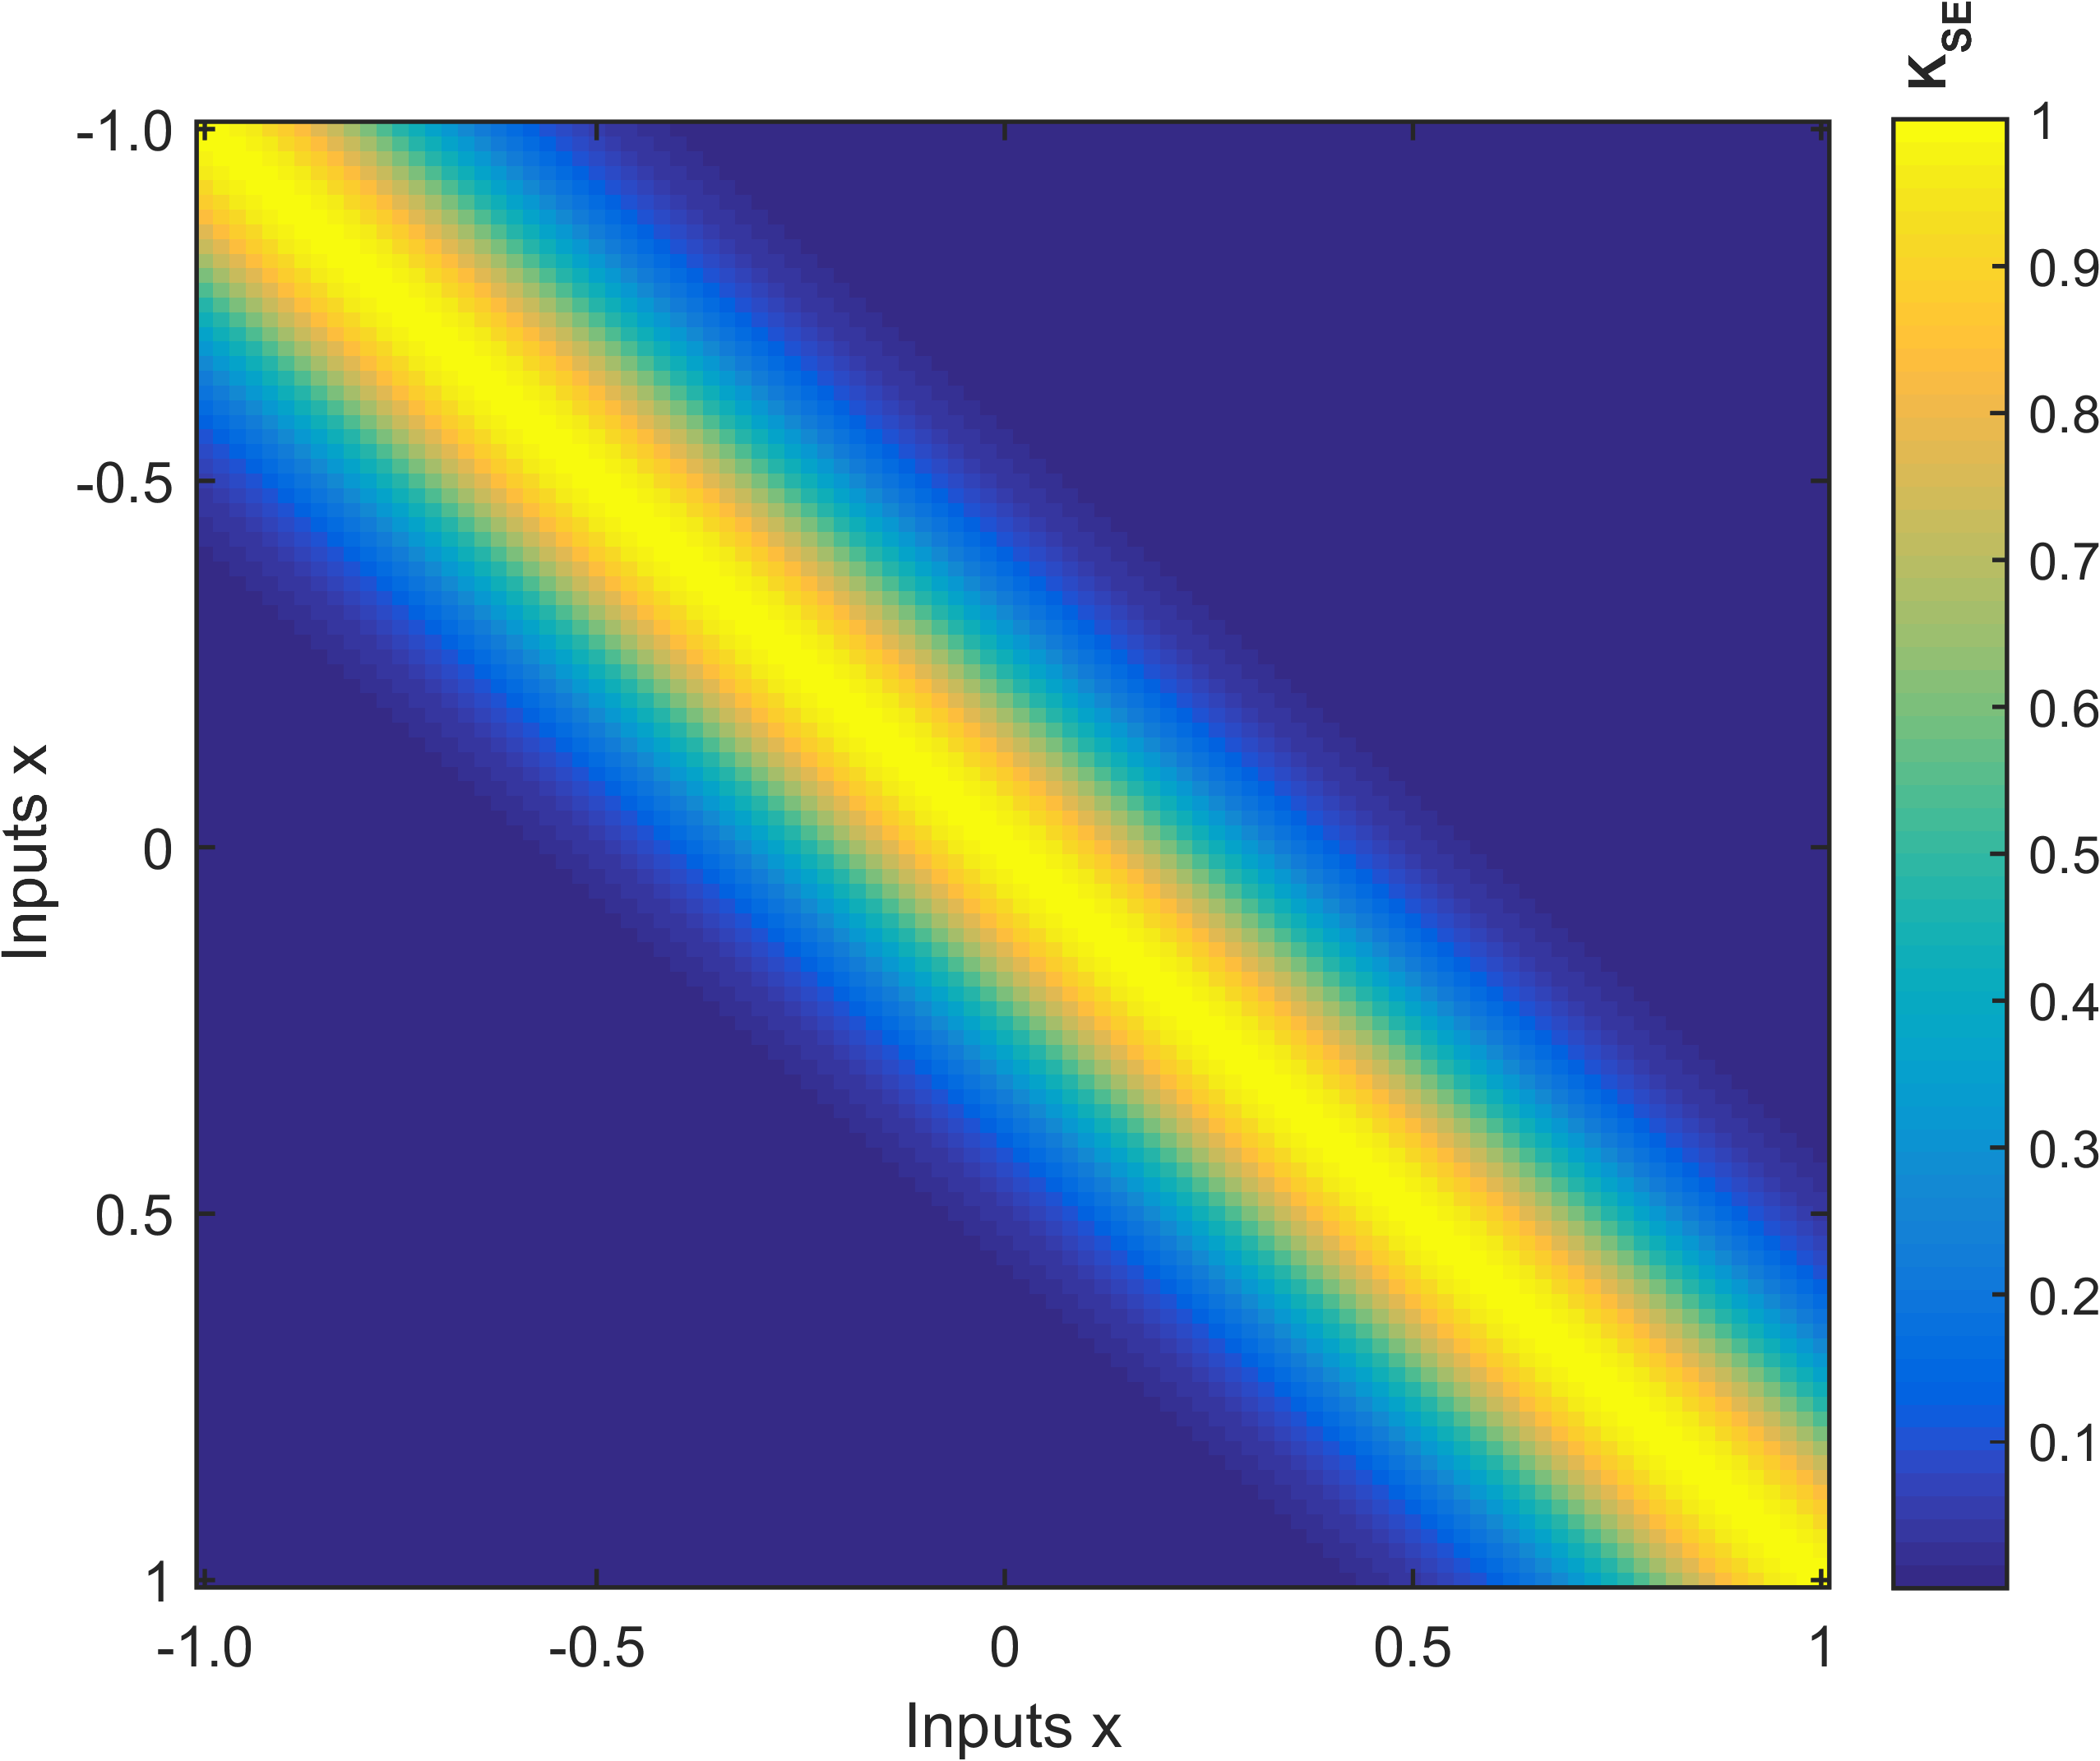
\includegraphics[width=0.45\textwidth]
        {images/covSEmatrix_1}
        \label{subFigcovSEmatrix_1}
  }\quad
\subfigure[{Covariance matrix for a Standard Exponential (SE) with $(\theta = [1, 0.5])$ at the input points $X^{*} = \{[0:0.02:1]\}$}]
  {
        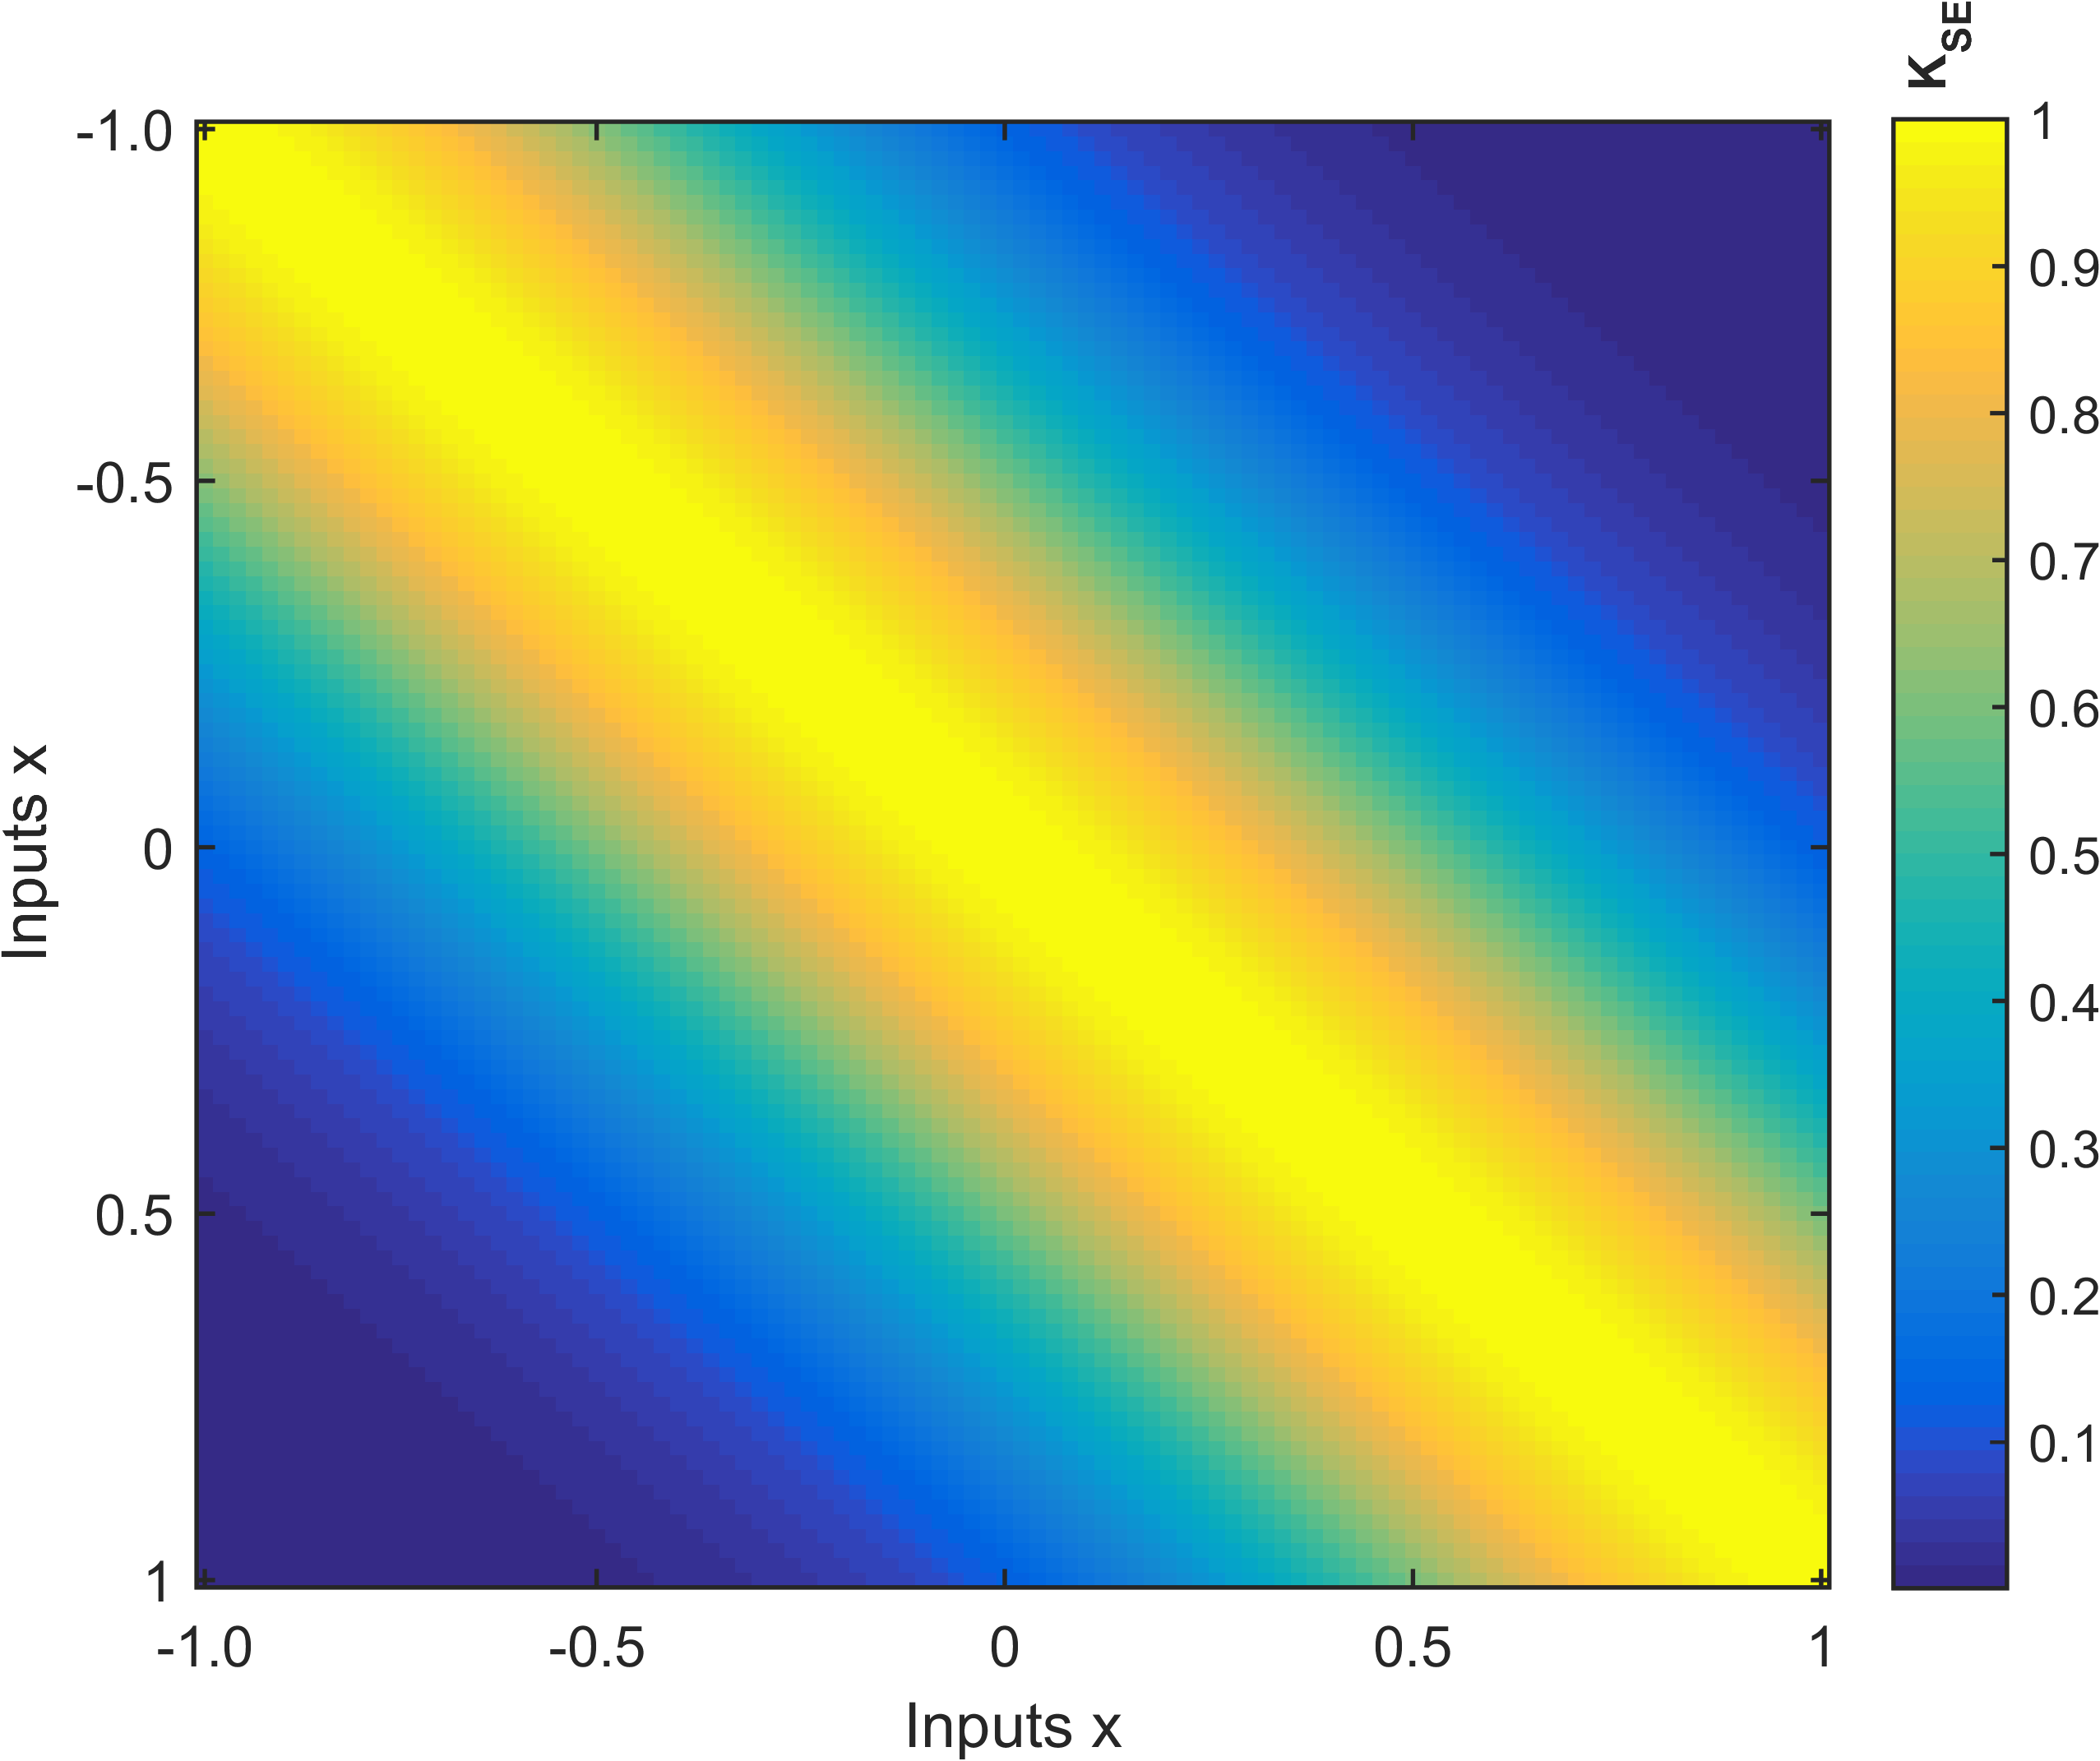
\includegraphics[width=0.45\textwidth]
        {images/covSEmatrix_2}
        \label{subFigcovSEmatrix_2}
  }\quad
  
       \caption{Covariance matrix for a Standard Exponential kernel with different hyper-parameters at the input points $X^{*} = \{[0:0.02:1]\}$. The SE kernel of figure \ref{subFigcovSEmatrix_1} has a lower length-scale than figure \ref{subFigcovSEmatrix_2}. Note, how the covariance values are more spread out for figure \ref{subFigcovSEmatrix_2}.}\label{figGPCovarianceMatrix}
\end{figure}

To generate a random Gaussian vector $f(X_{*})$ of length $N_{*}$, we first calculate the Cholesky decomposition\footnote{Cholesky Decomposition is also called the square-root of matrix and is defined for positive definite matrices} of the covariance matrix $K(X_{*}, X_{*}) = LL^{T}$, where $L$ is a lower triangular matrix. We then generate a random vector $U$, such that $U = \mathcal{N}(0, I)$ and $I$ is an identity matrix of size $N_{*}$.  The random vector can be then computed as, $f(X_{*}) = m(X_{*}) + LU$ and when plotted with the inputs $X_{*}$ gives a randomly drawn function. Figure \ref{figGPPriors} shows 5 random functions drawn for a zero mean GP with the covariance matrices of figure \ref{figGPCovarianceMatrix}. The solid black line defines the mean function, shaded blue region defines 95\% confidence interval (2$\sigma$) distance away from the mean. The dashed lines are five functions drawn at random from a GP prior. We can observe that figure \ref{subFigSEPrior_1} varies faster when compared to figure \ref{subFigSEPrior_2} due to smaller length scale hyper-parameter. 

\begin{figure}[!ht]
  \centering
    \subfigure[{Draws from a GP prior with mean zero and Standard Exponential (SE) Kernel with $(\theta = [1, 0.2])$. }]
  {
        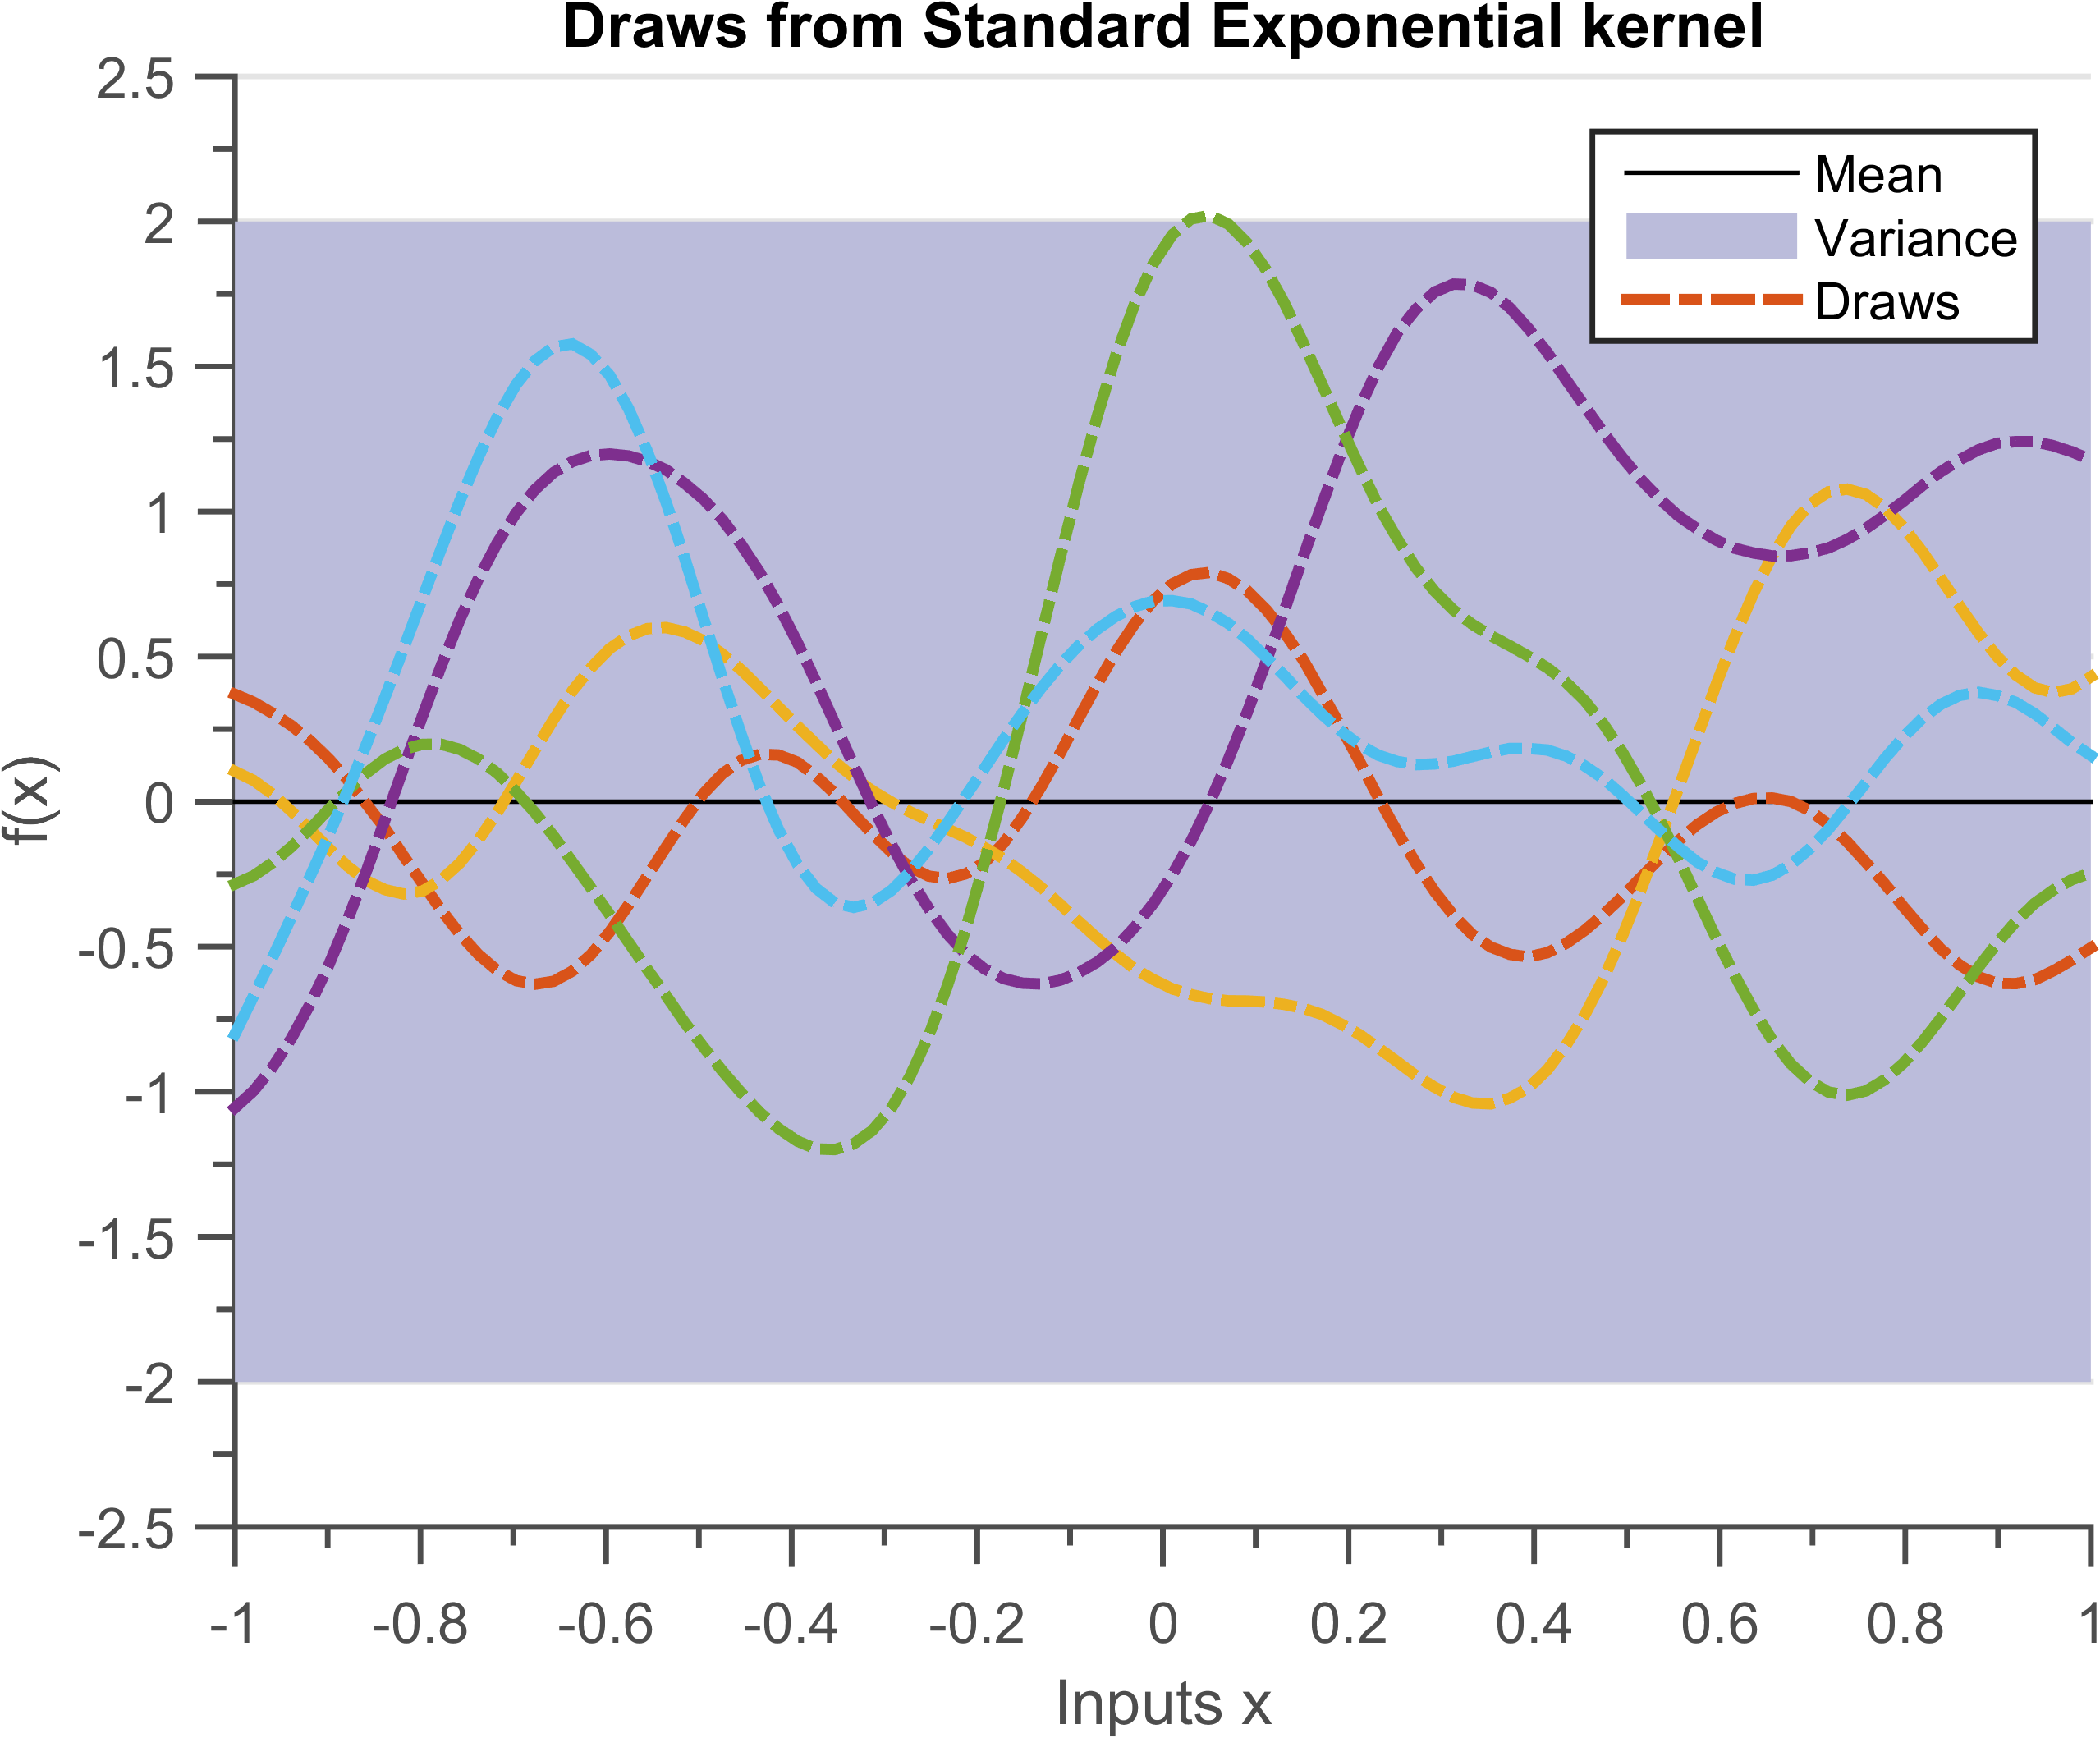
\includegraphics[width=0.45\textwidth]
        {images/drawsSEKernel_1}
        \label{subFigSEPrior_1}
  }\quad
\subfigure[{Draws from a GP prior with mean zero and Standard Exponential (SE) with $(\theta = [1, 0.5])$}]
  {
        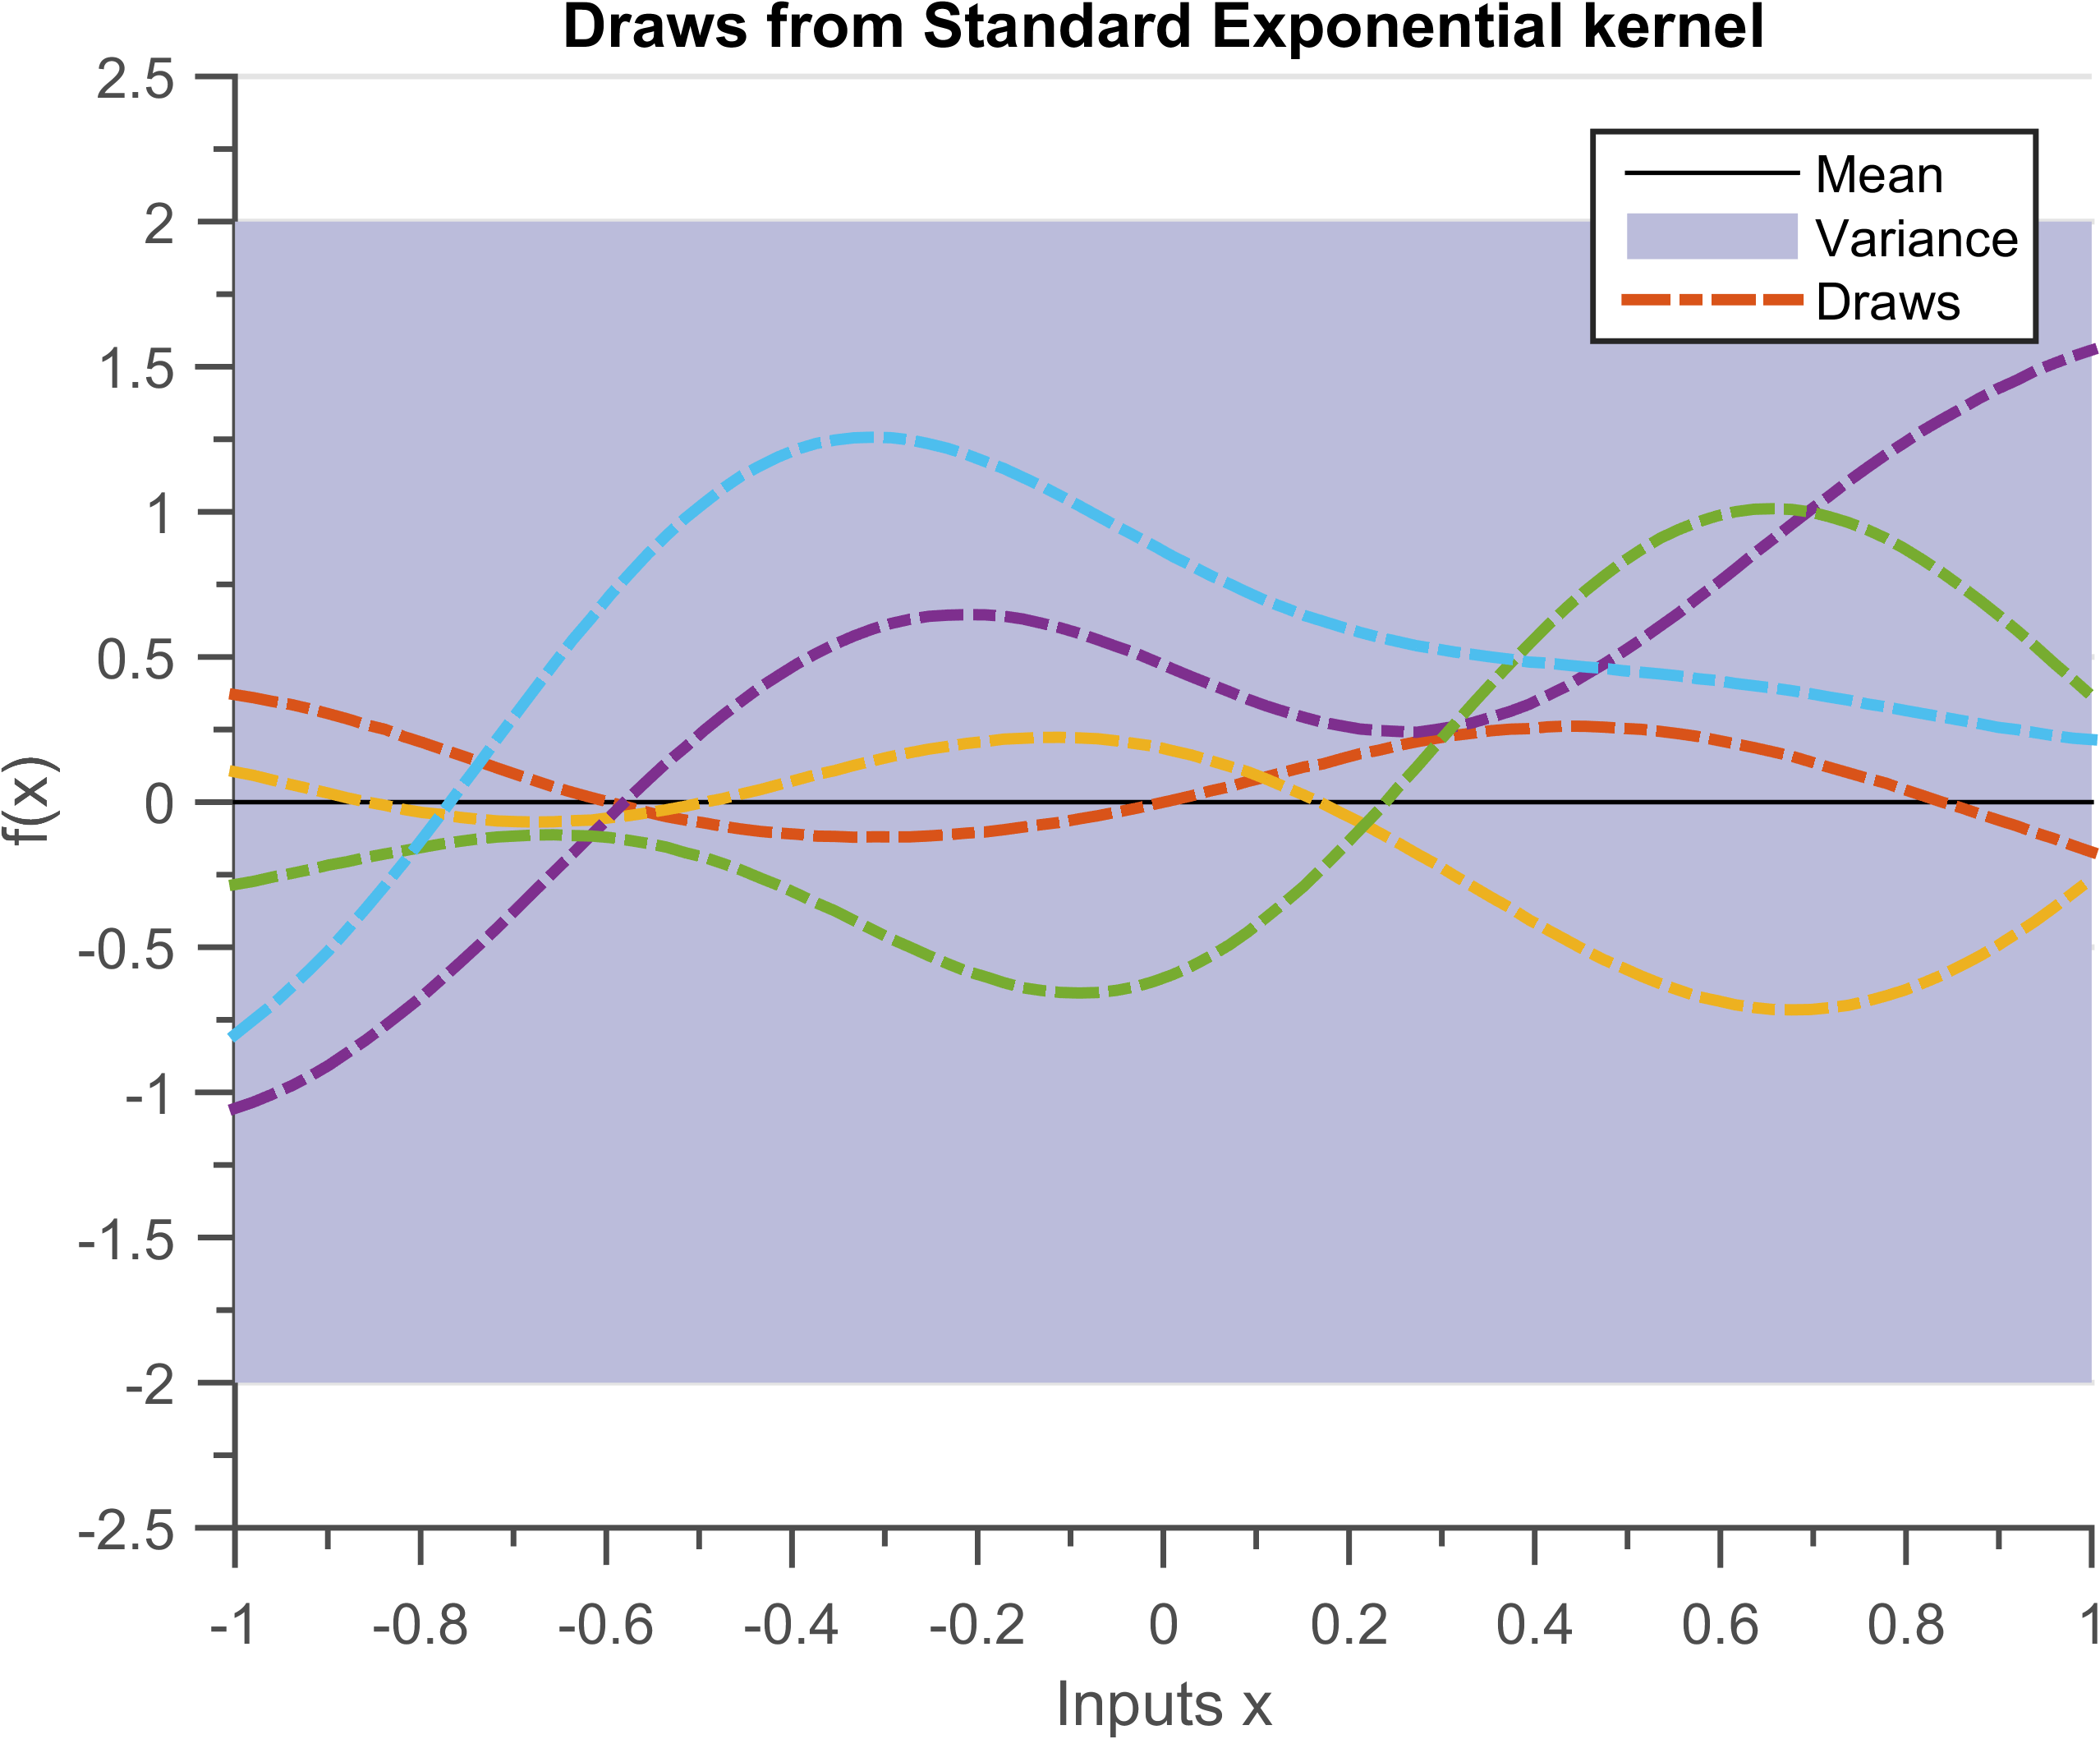
\includegraphics[width=0.45\textwidth]
        {images/drawsSEKernel_2}
        \label{subFigSEPrior_2}
  }\quad
  
       \caption{The solid black line defines the mean function, shaded blue region defines 95\% confidence interval (2$\sigma$) distance away from the mean. The dashed lines are five functions drawn at random from a GP prior. We can observe that figure \ref{subFigSEPrior_1} varies faster when compared to figure \ref{subFigSEPrior_2} due to smaller length scale hyper-parameter.       }\label{figGPPriors}
\end{figure}



\section{Posterior}\label{secPosterior}
Once we have defined an appropriate prior we wish to incorporate the information of training data set into the probabilistic framework. In the Bayesian framework, a posterior is the probability distribution after updating the information of evidence into prior knowledge. 


\subsection{Posterior with Noise-free observations}\label{subSecPosteriorNoiseFree}
We first consider the case of noise-free observations, that is we know $\{y(x_{i}) = f_{i} | i \in [1; N] \}$. This is case for many high-fidelity computer simulations, since high-fidelity computer simulations can be treated as having no noise \cite{sacks1989design}. If we desire to interpolate at $N_{*}$ test points $X_{*}$, then the multi-variate distribution of the training outputs $f(X)$ and test outputs $f(X_{*})$ according to the GP prior, test and training points is given by equation \ref{equationJointPriorNoiseFree}.

\begin{equation}\label{equationJointPriorNoiseFree}
\Pr\left [ \begin{matrix}
f(X)
\\ f(X_{*})
\end{matrix} \right ] = 
\mathcal{N}\left (\left [ \begin{matrix} 0 \\ 0 \end{matrix} \right ]
, 
\left [ \begin{matrix}
K(X, X) & K(X, X_{*})\\ 
K(X_{*}, X) & K(X_{*}, X_{*})
\end{matrix} \right ]
\right)
\end{equation}

$K(X, X_{*})$ is $N \times N_{*}$ covariance matrix between the training points $X$ and test points $X_{*}$ (equation \ref{eqnCovMatrixSquaredExponential}). The other covariance matrices $K(X, X)$, $K(X_{*}, X)$ and $K(X_{*}, X_{*})$ can be computed similarly. 

The posterior will be the the conditional probability of $f(X_{*})$ given the prior and data set. For a multi-variate Gaussian the conditional distribution is also a multi-variate Gaussian and can be calculated tractably, for a more detailed derivation refer to appendix \textbf{refer to the appendix here}. Graphically, we can imagine that the Bayes theorem is removing all the functions from our prior family of functions that do not pass through the data set (figure \ref{figGPNoiseLessPosteriors}). The predicted distribution after adding the information of data set into the prior can be written as:

  \begin{equation}\label{eqNoiseFreePosteriorGP}
  \begin{aligned}
  \Pr(f(X_{*}) \mid X_{*}, X, f(X)) = GP(  & K(X_{*}, X)( K(X, X) )^{-1}f(X),   \\ 
                                & K(X_{*}, X_{*}) - K(X_{*}, X)( K(X, X) )^{-1} K(X, X_{*}))
  \end{aligned}
  \end{equation}

The term $K(X_{*}, X)( K(X, X) )^{-1}f(X)$ is the predicted mean of the posterior at the test points $X_{*}$. The term $K(X_{*}, X_{*}) - K(X_{*}, X)( K(X, X) )^{-1} K(X, X_{*})$ is the predicted covariance. 

\textbf{define $\mathcal{D}_{2}$}


\begin{figure}[!ht]
  \centering
    \subfigure[{Posterior distribution for the case of noiseless observations. Prior is a GP with mean zero and covariance as Standard Exponential (SE) Kernel with $(\theta = [1, 0.2])$, data set is $\{x = -0.5; f = 0\}$.}]
  {
        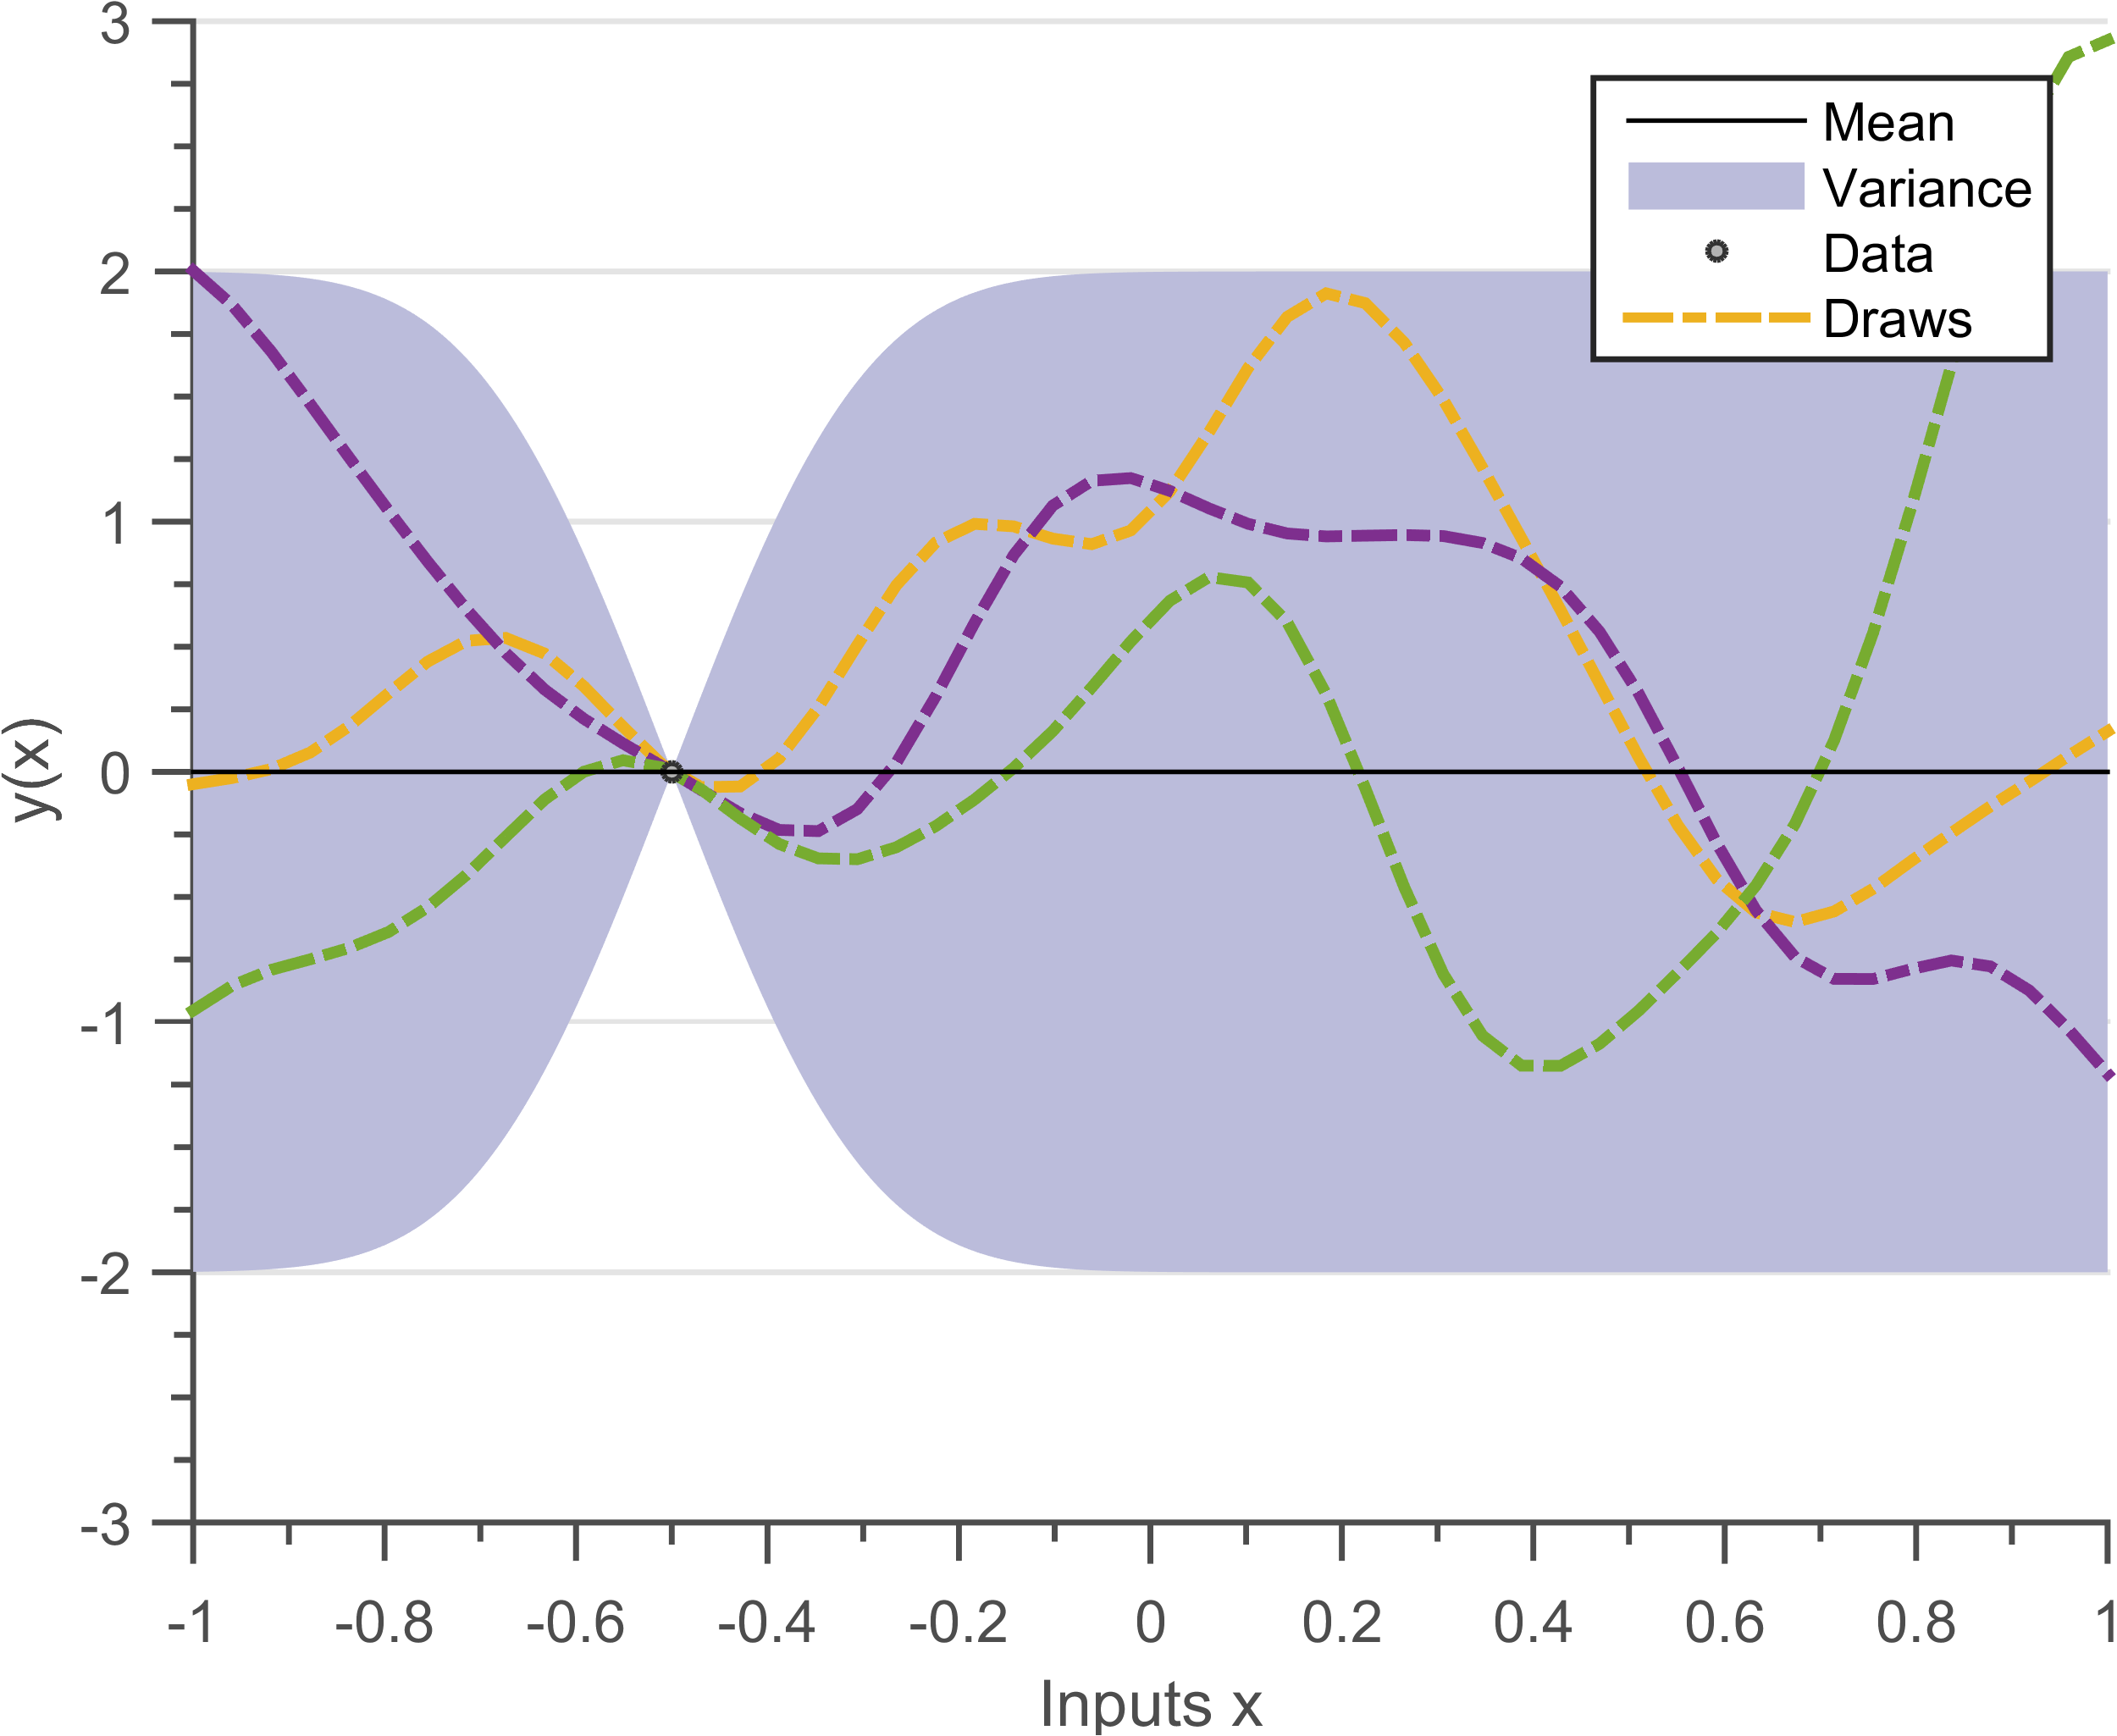
\includegraphics[width=0.45\textwidth]
        {images/posteriorSENoiseLess_1}
        \label{posteriorSENoiseLess_1}
  }\quad
\subfigure[{Posterior distribution for the case of noiseless observations. Prior is a GP with mean zero and covariance as Standard Exponential (SE) Kernel with $(\theta = [1, 0.2])$, data set is $\{x = [-0.5, 0.33, 0.66]; f = [0, 0.5, 0.5]\}$}.  ]
  {
        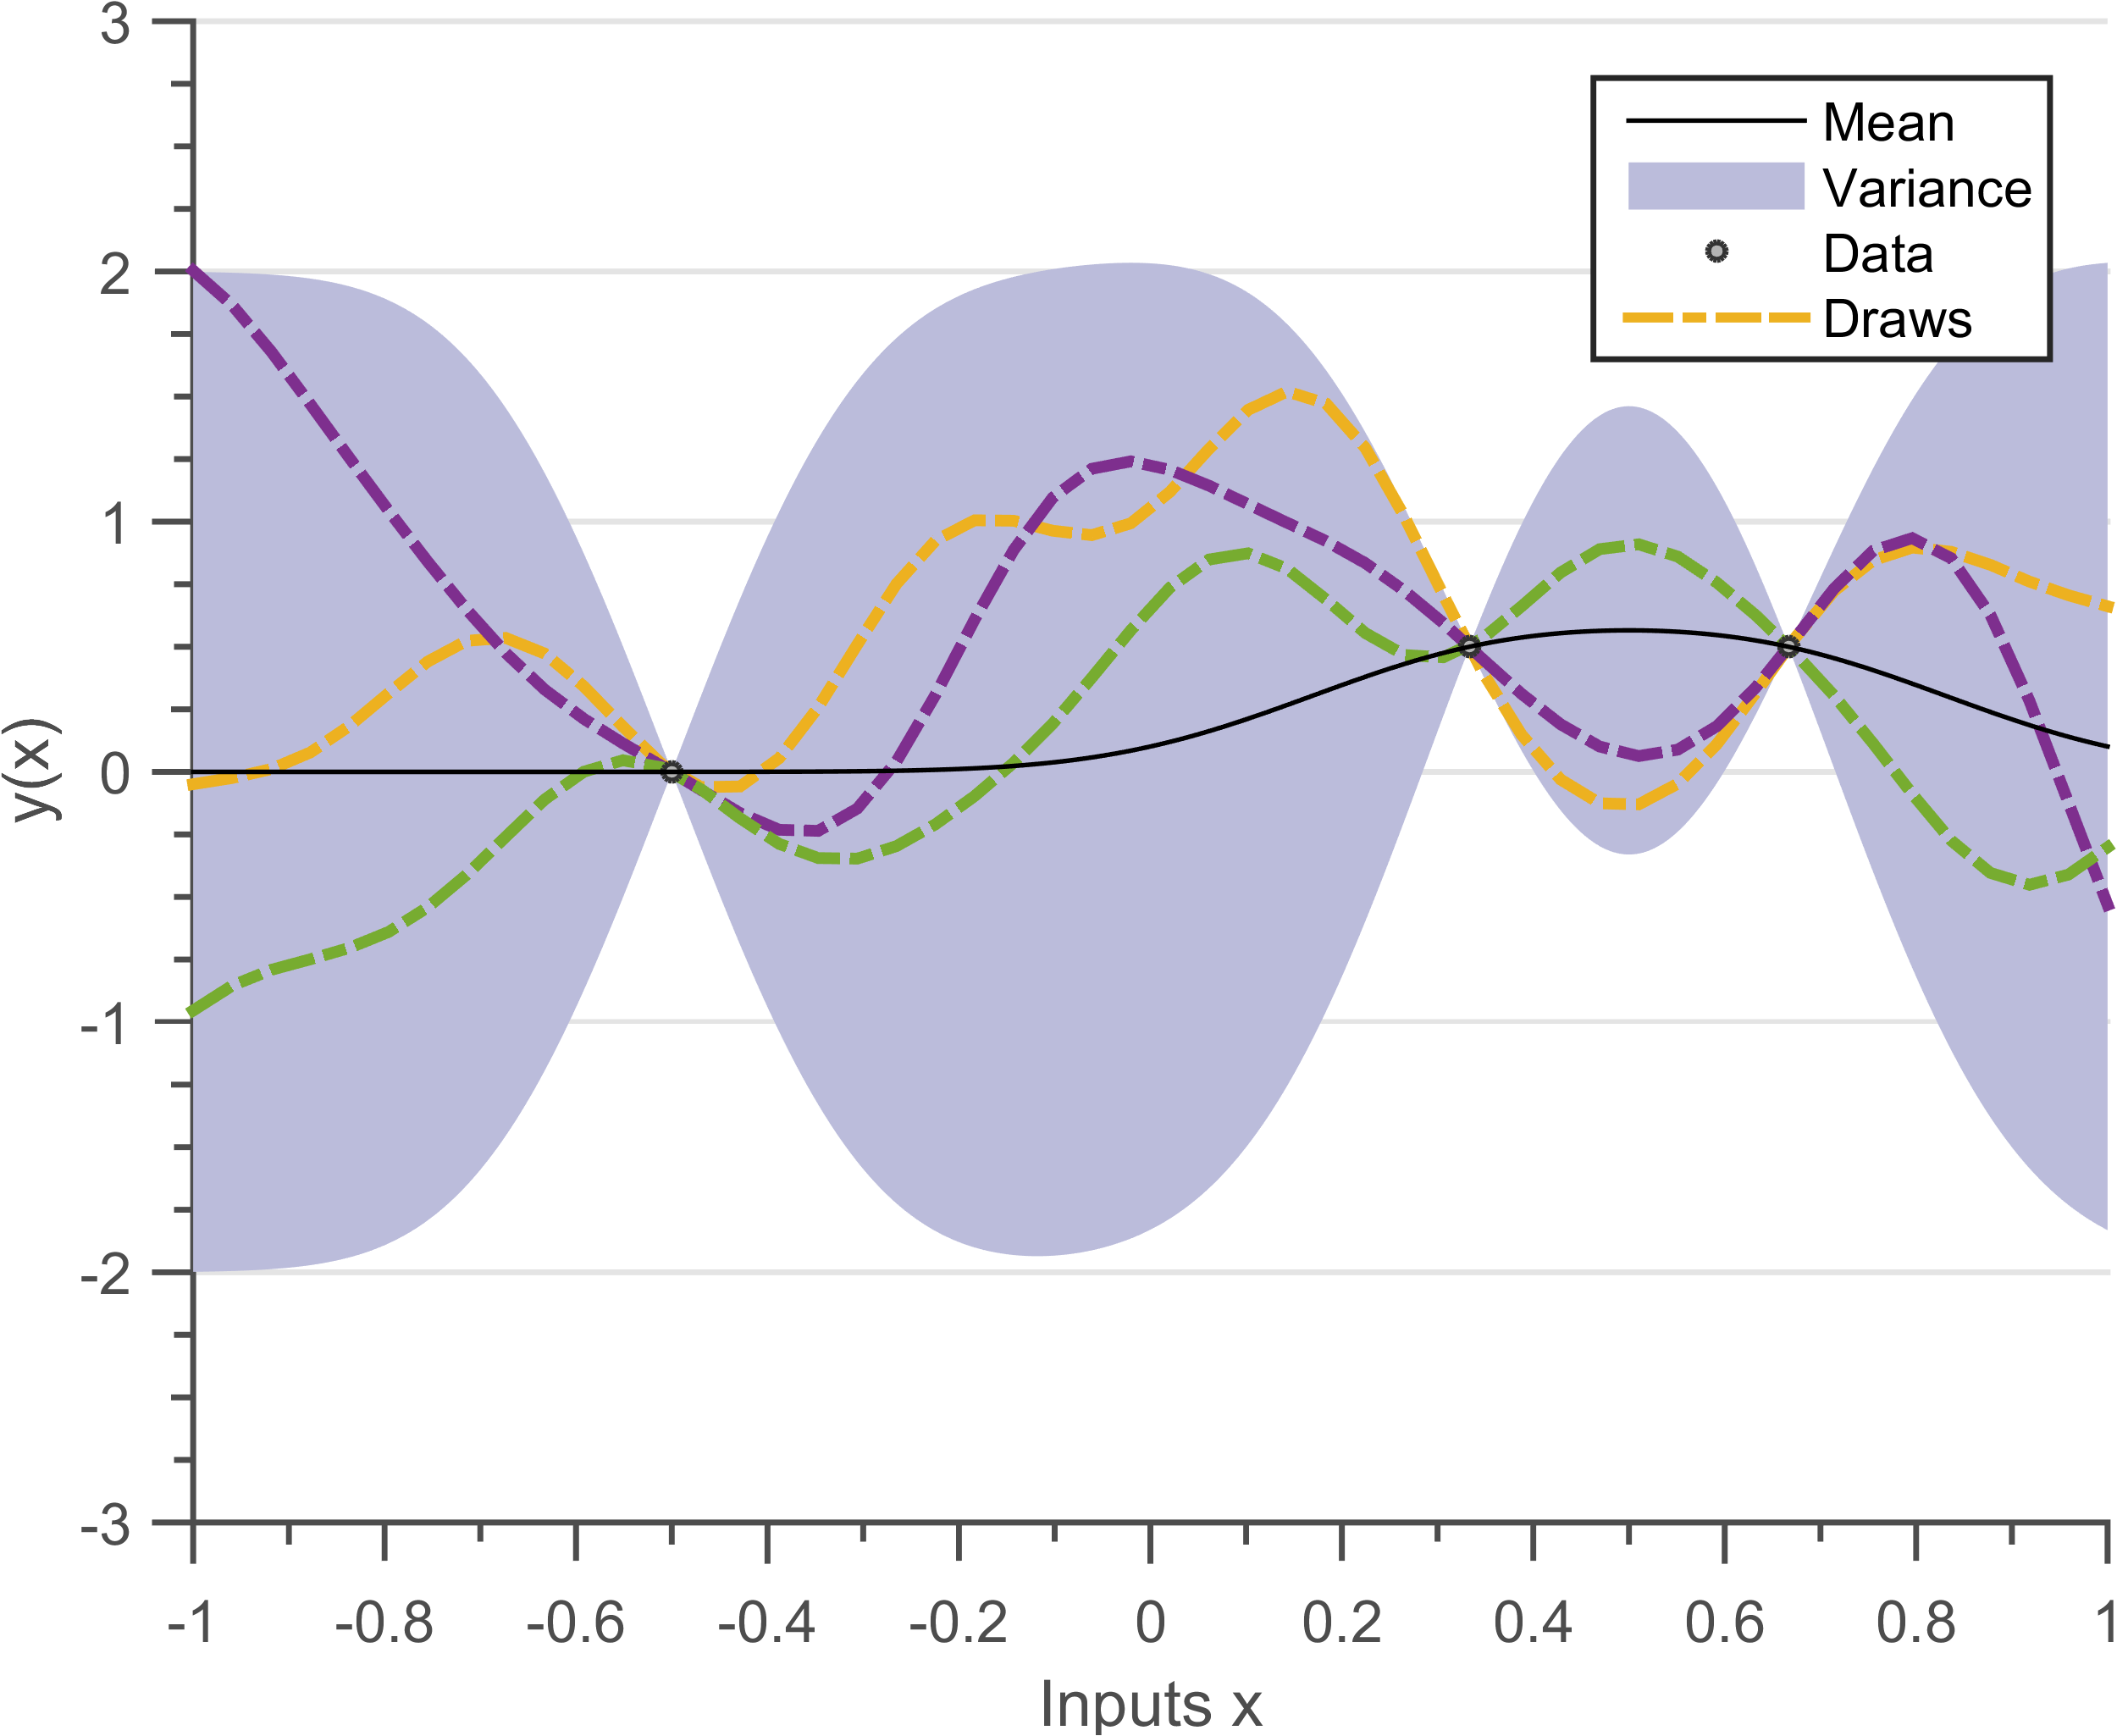
\includegraphics[width=0.45\textwidth]
        {images/posteriorSENoiseLess_3}
        \label{posteriorSENoiseLess_3}
  }\quad
  
       \caption{Prediction in the case of noiseless observations. The solid black line defines the mean function, blue region defines 95\% confidence interval (2$\sigma$) distance away from the mean. The dashed lines are three functions drawn at random from a GP posterior. We can observe that Bayes Theorem eliminates all the functions that do not pass through the observed data-set.}
       \label{figGPNoiseLessPosteriors}
\end{figure}

Figure \ref{figGPNoiseLessPosteriors} shows the posterior GP after adding observed data into the initial prior. We can see that Bayes theorem eliminates all the functions in the prior that does not pass through the data. The solid black line defines the mean function, blue region defines 95\% confidence interval (2$\sigma$) distance away from the mean. The mean of the of the posterior distribution is also used as a point estimate for interpolation. The dashed lines are three functions drawn at random from a GP posterior. Random functions can be sampled from the posterior distribution as described in the earlier section. 

\subsection{Posterior with Noisy observations}\label{subSecPosteriorNoisy}
If we assume a more general case of noisy observations then the measured outputs can be written as:

\begin{equation}\label{eqNoiseEquation}
y(x) = f(x) + \epsilon
\end{equation}

Such that $\epsilon$ is an independent random noise sampled from a white noise Gaussian $\mathcal{N}(0, \sigma_{n}^{2})$. We can thus write the prior GP of the noisy case as:

\begin{equation}\label{equationMeanZeroGPNoisydefinition}
\Pr[y(x) \mid X, \sigma_{n}] = GP(0 , k(x_{1}, x_{2}) + \sigma^{2}_{n}\delta_{xx'})
\end{equation}

Here, $\delta_{xx'}$ is a Kronecker delta which is one iff $x = x'$ and zero otherwise. Since the noise is independent for each observation hence there is no noise term for covariances between inputs. The joint distribution of the training outputs $Y(X)$ and true physical process $f(X_{*})$ according to the above prior becomes:

\begin{equation}\label{equationJointPriorNoisy}
\Pr\left [ \begin{matrix}
Y(X)
\\ f(X_{*})
\end{matrix} \right ]
= 
\mathcal{N}\left (
\left [ \begin{matrix}
0
\\ 0

\end{matrix} \right ] , \left [ \begin{matrix}
K(X, X) + \sigma^{2}_{n}I & K(X, X_{*})\\ 
K(X_{*}, X) & K(X_{*}, X_{*})
\end{matrix} \right ] 
\right )
\end{equation}

The difference between equation \ref{equationJointPriorNoisy} and \ref{equationJointPriorNoiseFree} is the addition of noise term $\sigma^{2}_{n}I$. The noise is assumed to be independent hence is multiplied to an identity matrix, to know how to add more complex noise models please refer to chapter \ref{chapBasicCovarianceKernels}. The posterior distribution of $f(X_{*})$ can be calculated as:

  \begin{equation}\label{eqNoisyPredictiveGP}
  \begin{aligned}
      \Pr(f(X_{*}) \mid X_{*}, X, Y(X)) = GP(  & K(X_{*}, X)( K(X, X) + \sigma^{2}_{n}I)^{-1}f(X),   \\ 
                                & K(X_{*}, X_{*}) - K(X_{*}, X)( K(X, X) + \sigma^{2}_{n}I)^{-1} K(X, X_{*}) 
  \end{aligned}
  \end{equation}

Figure \ref{figGPNoisyPosteriors} shows the posterior GP after adding observed data into the initial prior. The solid black line defines the mean function, blue region defines 95\% confidence interval (2$\sigma$) distance away from the mean. The dashed lines are three functions drawn at random from a GP posterior. Random functions can be sampled from the posterior distribution as described in the earlier section \ref{secPrior}.  Due to the inclusion of noise in the prior, we see that the draws from posterior are not necessarily passing from the observed point.

\begin{figure}[!ht]
  \centering
    \subfigure[{Posterior distribution for the case of noisy observations. Prior is a GP with mean zero, covariance as Standard Exponential (SE) Kernel with $(\theta = [1, 0.2])$ and noise as $\sigma_{n} = [0.02])$, , data set is $\{x = -0.5; f = 0\}$.}]
  {
        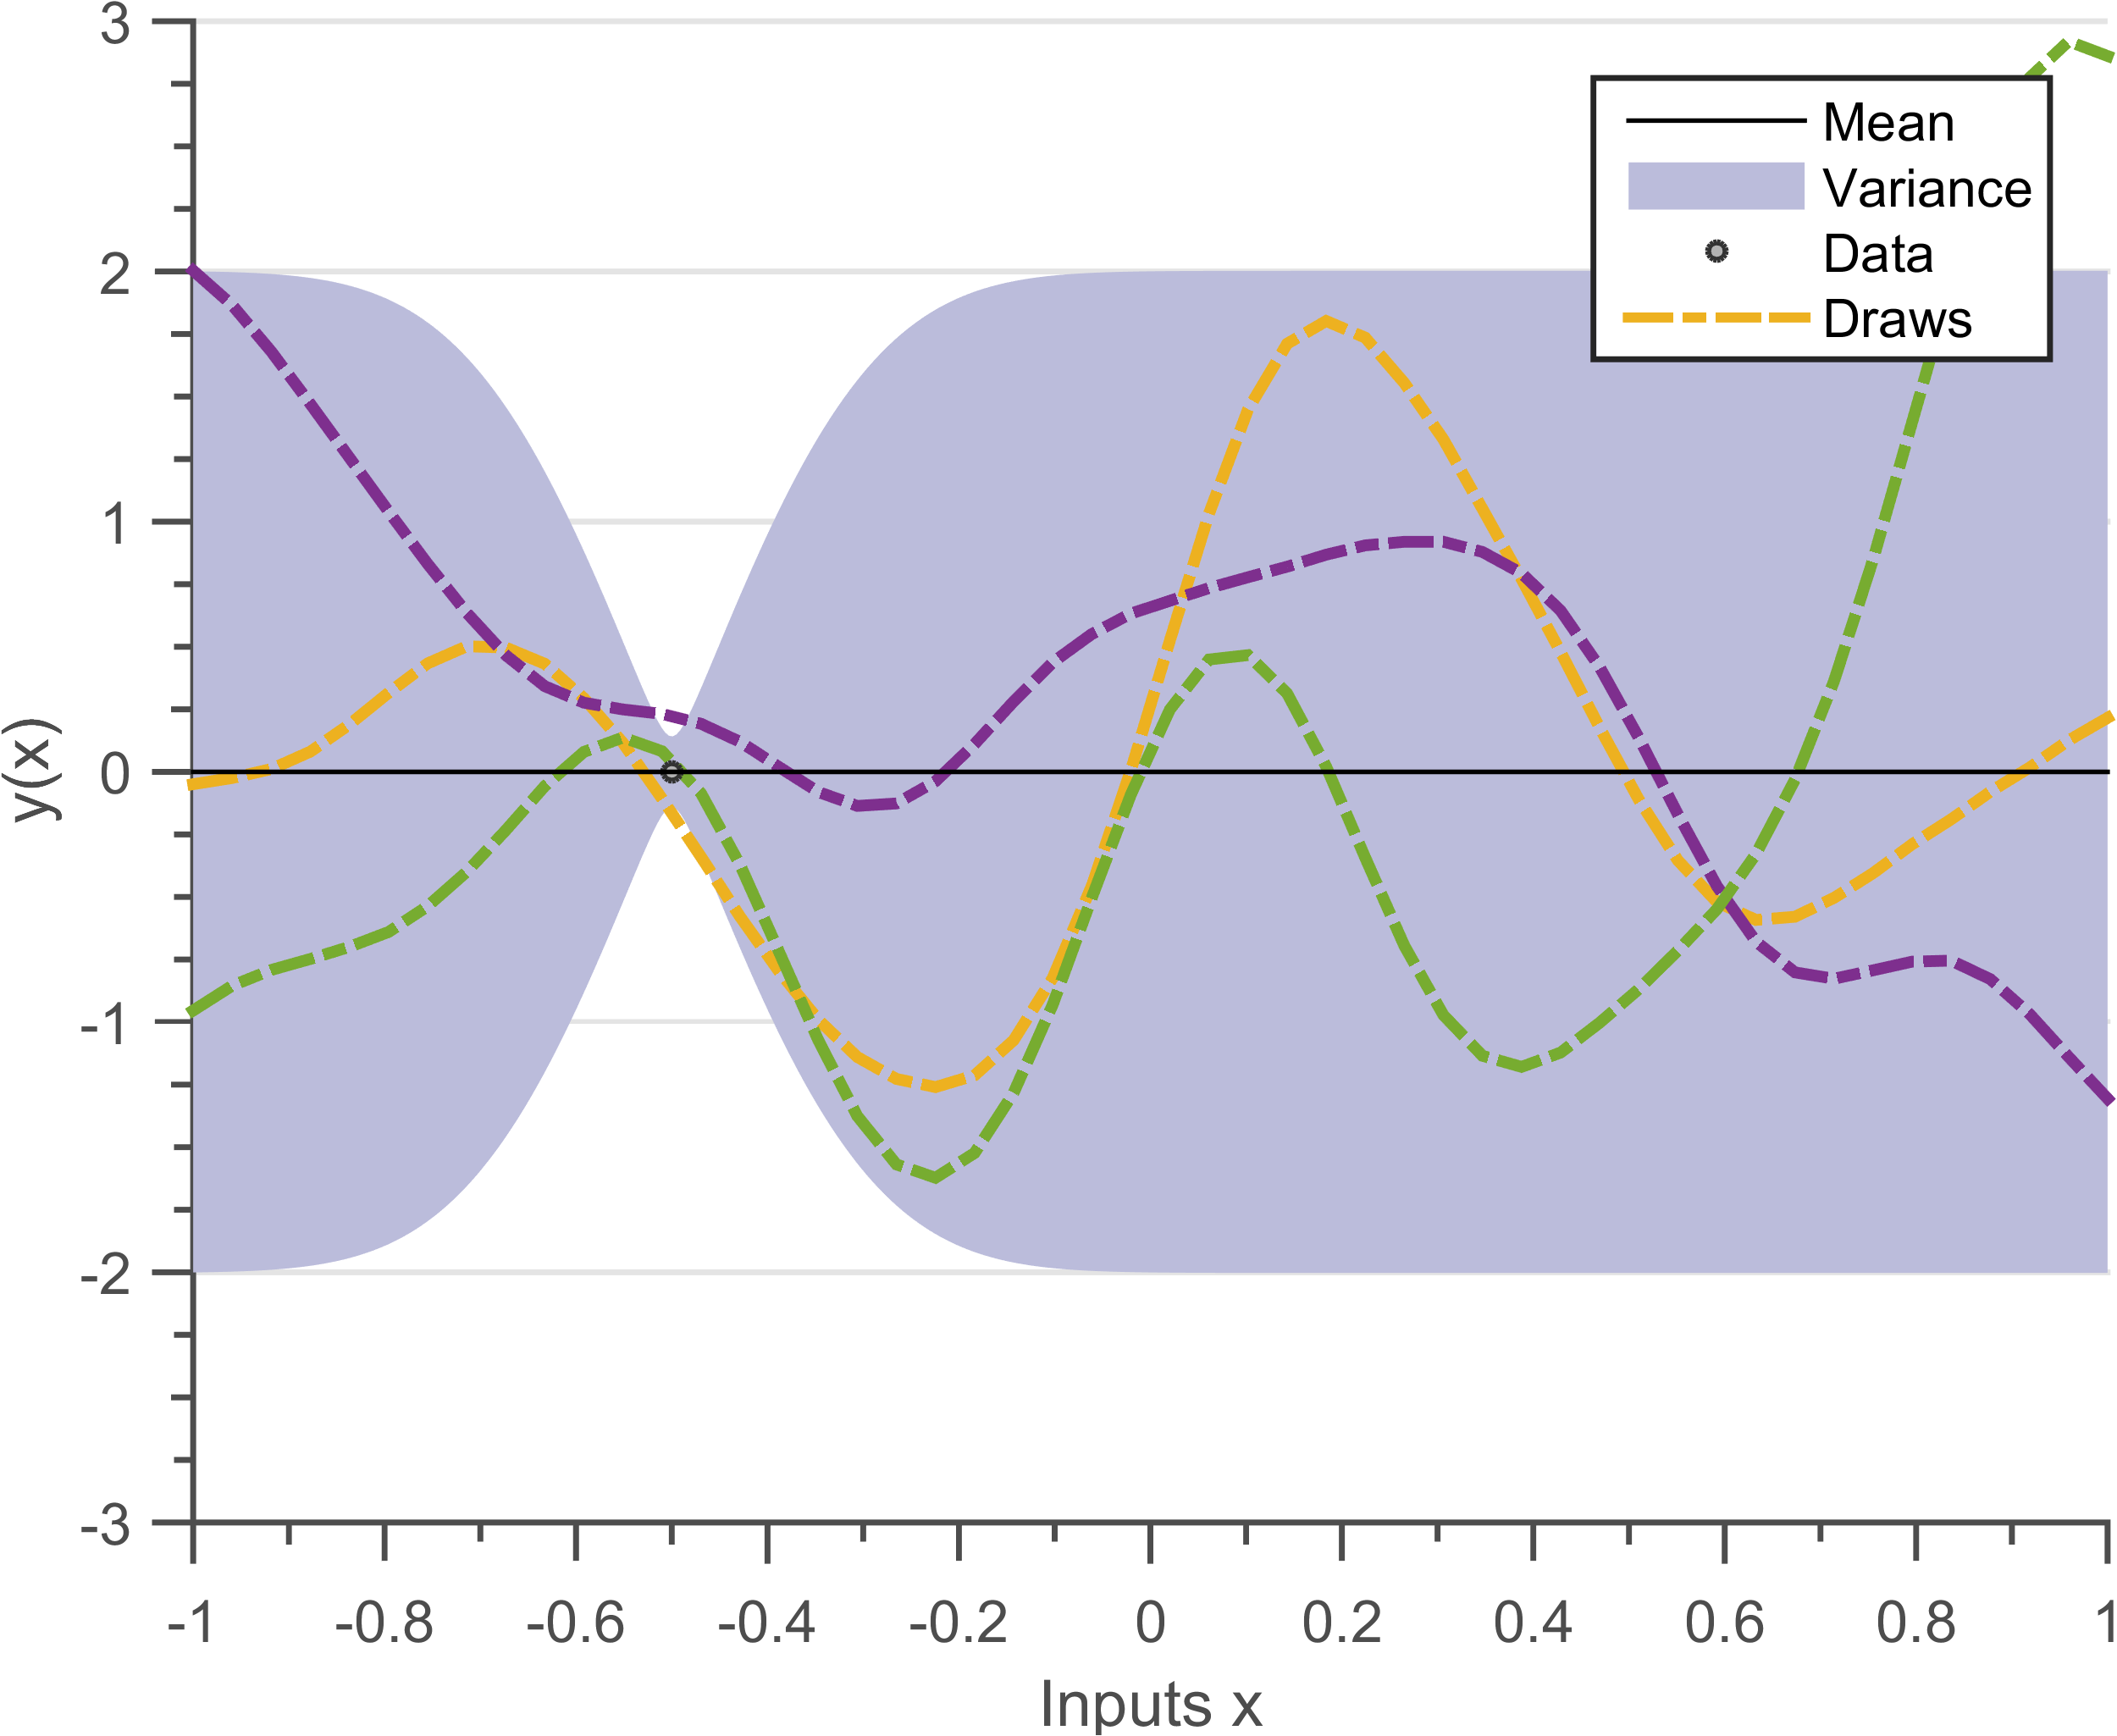
\includegraphics[width=0.45\textwidth]
        {images/posteriorSENoisy_1}
        \label{posteriorSENoisy_1}
  }\quad
\subfigure[{Posterior distribution for the case of noisy observations. Prior is a GP with mean zero, covariance as Standard Exponential (SE) Kernel with $(\theta = [1, 0.2])$ and noise as $\sigma_{n} = [0.02])$, , data set is $\{x = [-0.5, 0.33, 0.66]; f = [0, 0.5, 0.5]\}$.}]
  {
        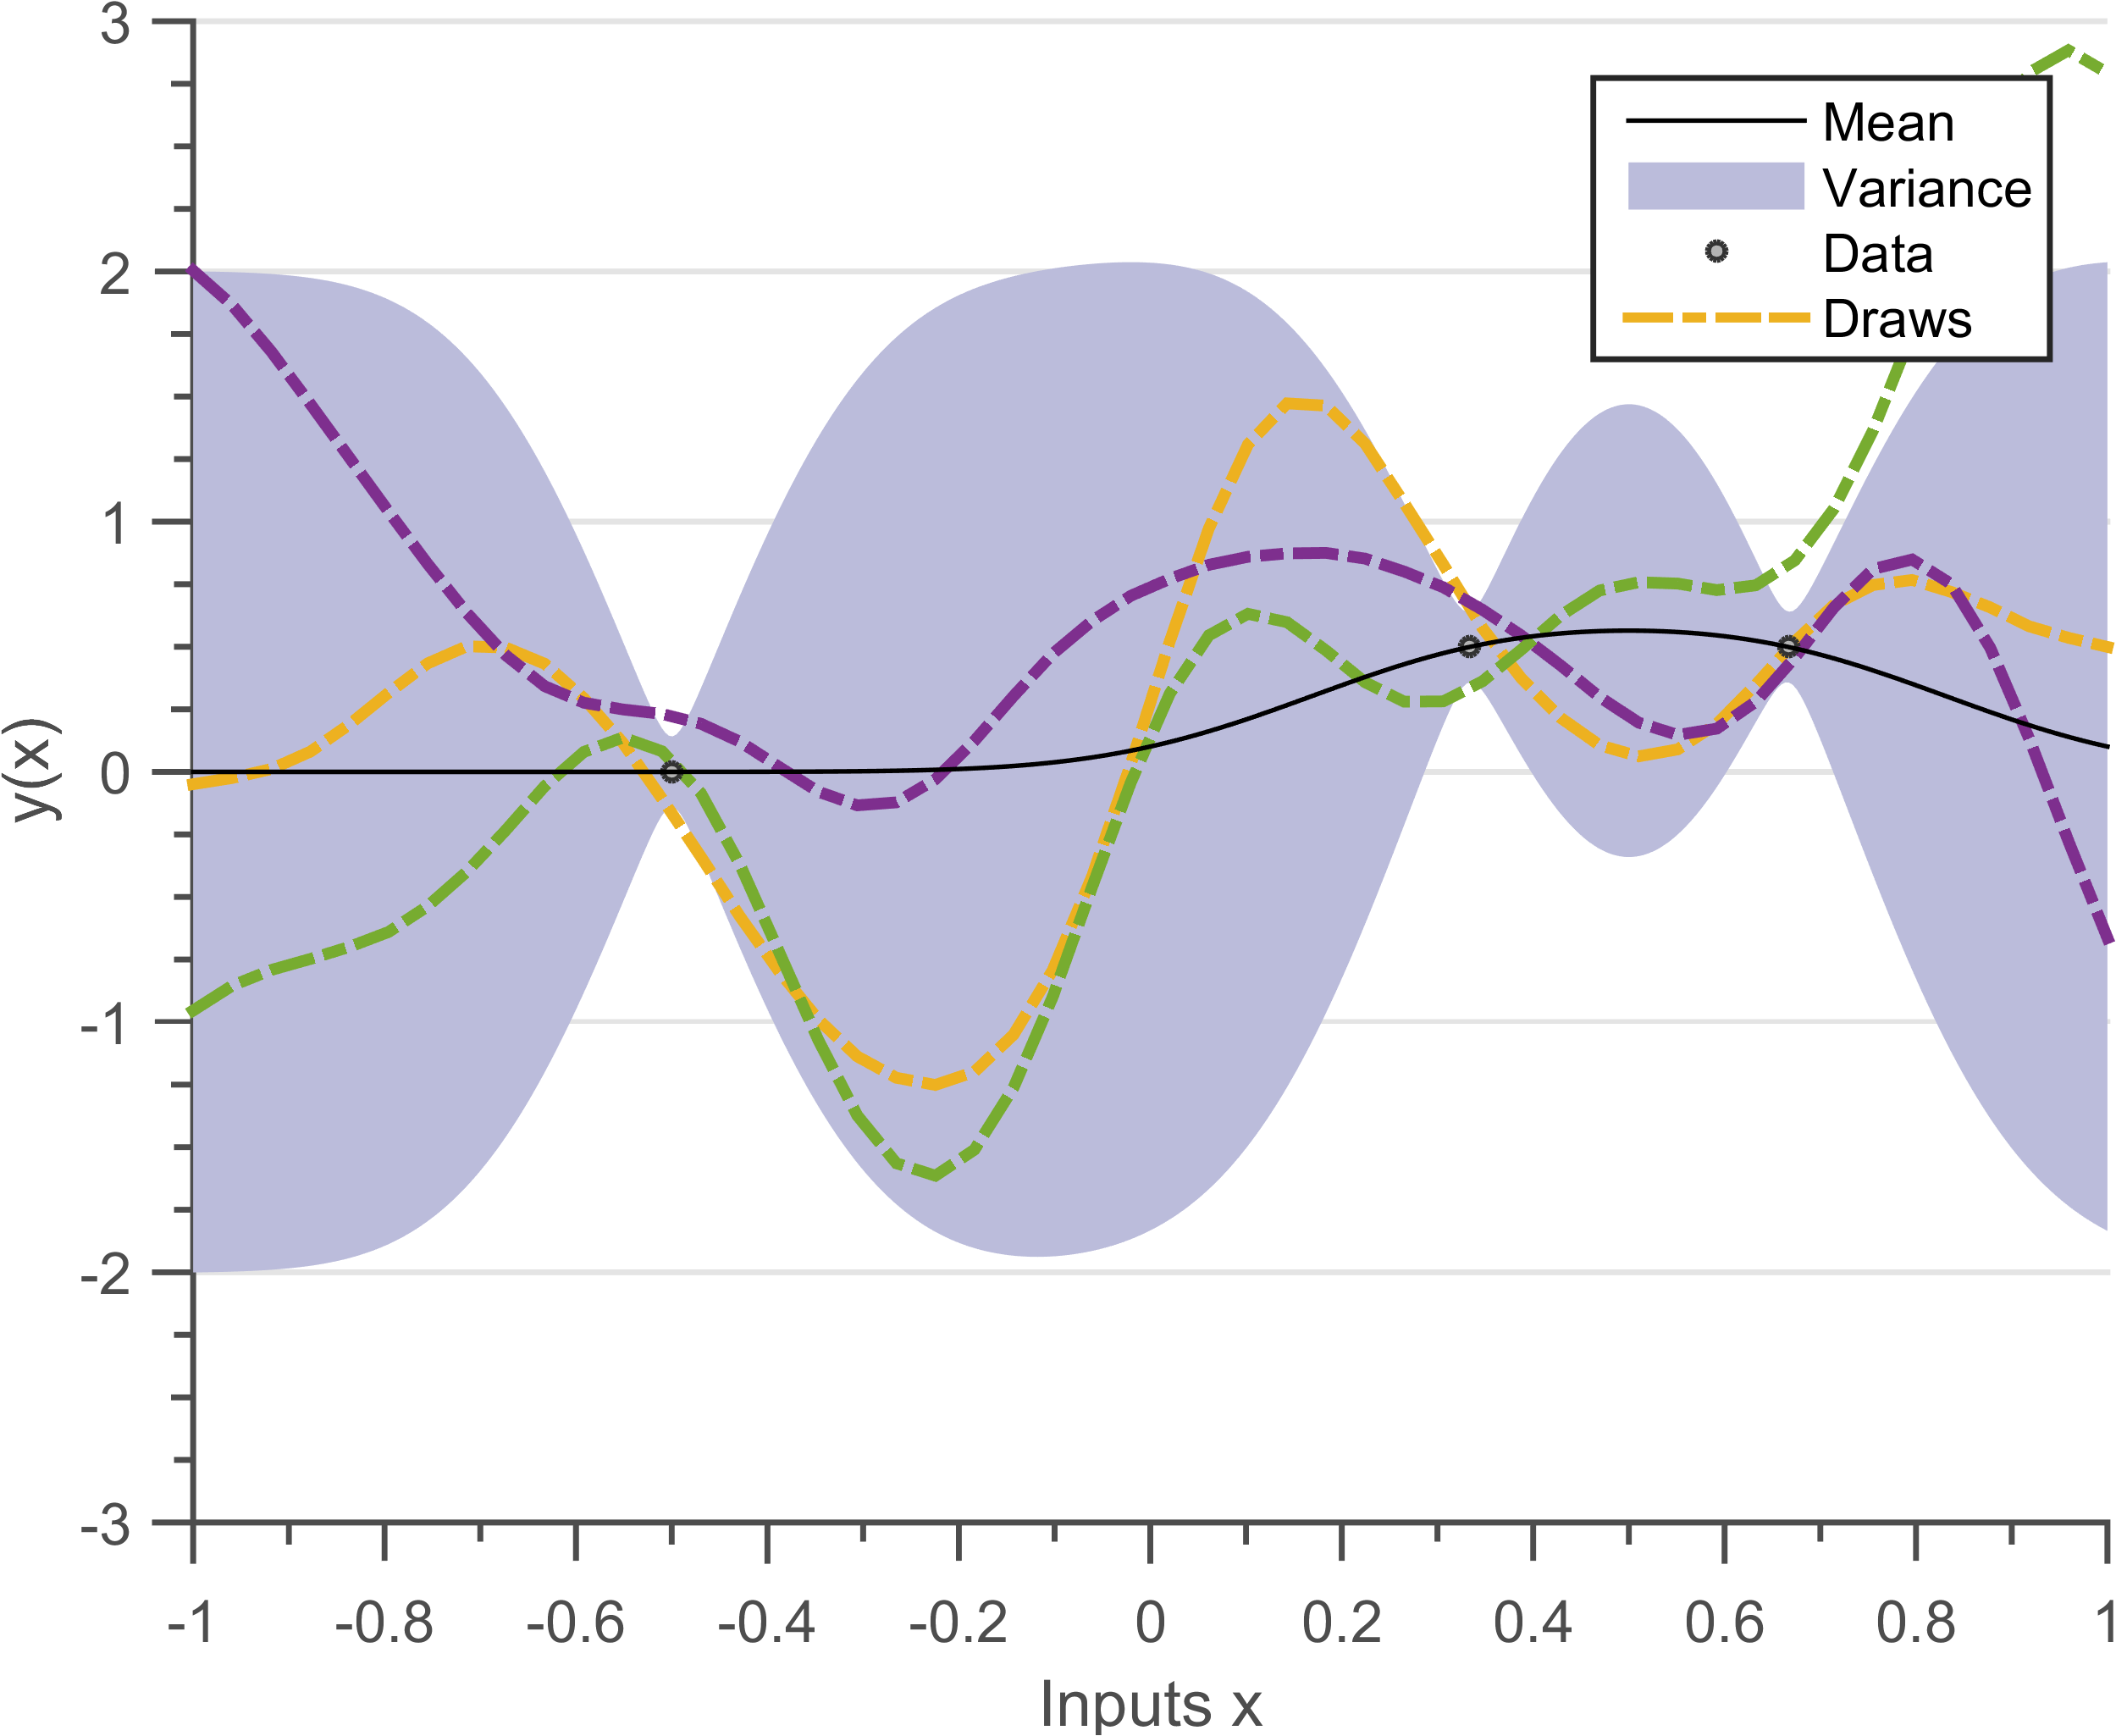
\includegraphics[width=0.45\textwidth]
        {images/posteriorSENoisy_3}
        \label{posteriorSENoisy_3}
  }\quad
  
       \caption{Prediction in the case of noisy observations. The solid black line defines the mean function, blue region defines 95\% confidence interval (2$\sigma$) distance away from the mean. The dashed lines are three functions drawn at random from a GP posterior. The mean and the draws do not pass exactly from the observation point.}
       \label{figGPNoisyPosteriors}
\end{figure}

\subsection{Interpretation of posterior}
We will now introduce a short hand notation and replace the lengthy notation $K(X, X)$ with $K_{XX}$ and $K(X, X_{*})$ with $K_{XX_{*}}$. For the case when we have only one test point $x_{*}$ we can write the predictive mean and variance in short-hand as:

  \begin{equation}\label{eqNoisyPredictiveMean}
  \mathbf{E}[f(x_{*})] = K_{Xx_{*}}^{T}( K_{XX} + \sigma^{2}_{n}I)^{-1}Y
  \end{equation}
  \begin{equation}\label{eqNoisyPredictiveCovariance}
	Cov[f(x_{*})] = K_{x_{*}x_{*}} - K_{Xx_{*}}^{T}( K_{XX} + \sigma^{2}_{n}I )^{-1} K_{Xx_{*}}
  \end{equation}

\paragraph{Precision Matrix}  
Both the predictive mean (equation \ref{eqNoisyPredictiveMean}) and predictive covariance (equation \ref{eqNoisyPredictiveCovariance}) need inverse of the covariance matrix $( K_{XX} + \sigma^{2}_{n}I)^{-1}$. The inverse of a covariance matrix is also known as a precision matrix. While the elements of a covariance matrix capture the variance and correlation information, a precision matrix contains the conditional dependence information \cite{mackay2003information}. Thus, if the $(i, j)^{th}$ element of a precision matrix is zero, the $i^{th}$ and $j^{th}$ random variables are conditionally independent. 

Calculating the precision matrix is a $\mathcal{O}\left ( N^{3} \right )$ operation for a covariance matrix of size $N$. After $N \sim 10,000$ a normal computer runs out of RAM and we thus cannot perform the inversion. Fortunately, there exist several approximations to efficiently inverse the covariance matrix and perform predictions, details are available in section \ref{chapScalingGPR}.

\paragraph{Predicted mean}
The predictive mean is a linear combination of the observations $y_{i}$, and has participation-factor of $K_{Xx_{*}}^{T}( K_{XX} + \sigma^{2}_{n}I)^{-1}$. For a SE kernel $K_{Xx_{*}}^{T}$ decreases exponentially with distance, hence observations closer to $x_{*}$ have more impact on the final prediction (equation \ref{eqNoisyPredictiveMeanLinearInY}). 
  
  \begin{equation}\label{eqNoisyPredictiveMeanLinearInY}
  \mathbf{E}[f(x_{*})] = \sum_{i = 1}^{N} K_{Xx_{*}}^{T}( K_{XX} + \sigma^{2}_{n}I)^{-1}y_{i}
  \end{equation}

The predictive mean can also be interpreted as a linear combination of the basis functions $K_{x_{i}x_{*}}$, and participation factors $( K_{XX} + \sigma^{2}_{n}I)^{-1}Y$ (equation \ref{eqNoisyPredictiveMeanLinearInBasis}). 

  \begin{equation}\label{eqNoisyPredictiveMeanLinearInBasis}
  \mathbf{E}[f(x_{*})] = \sum_{i = 1}^{N} K_{x_{i}x_{*}}( K_{XX} + \sigma^{2}_{n}I)^{-1}Y
  \end{equation}
  
This means that even though a GP represents of an infinite-dimensional vector (function), we only care about the $N$ dimensional multivariate Gaussian (section \ref{equationJointPriorNoisy}) to actually predict the mean. If the precision matrix is cached, then calculating the mean is an $\mathcal{O}\left ( N \right )$ operation.

\paragraph{Predicted variance}
The predictive variance is a combination of two terms $K_{x_{*}x_{*}}$ which is the variance due to prior assumptions and $- K_{Xx_{*}}^{T}( K_{XX} + \sigma^{2}_{n}I )^{-1} K_{Xx_{*}}$ which denotes the decrease in variance due to observations. The predictive distribution of test targets $y(x_{*})$ can be calculated by adding a noise term $\sigma^{2}_{n}$ in predictive covariance equation \ref{eqNoisyPredictiveCovariance}. 

  \begin{equation}\label{eqNoisyPredictiveCovarianceOnNoisyTarget}
	Cov[y(x_{*})] = K_{x_{*}x_{*}} - K_{Xx_{*}}^{T}( K_{XX} + \sigma^{2}_{n}I )^{-1} K_{Xx_{*}} + \sigma_{n}^{2}
  \end{equation}
  
We observe that the predicted variance in not dependent on the observations $y$, this is one of the flaws in GP regression. Since the assumption that the dataset $(\mathcal{D})$ comes from a GP might not necessarily be true, the predicted variance can poorly represent the model error. Hence, predicted variance is not necessarily a measure of model error but an efficient method to track uncertainties arising from the prior assumption and non-continuous observations \cite{shah2014student}.

The mean and variance are highly dependent on the kernel hyper-parameters. In order to automatically learn the hyper-parameters, we must perform model selection. Section \ref{secHyperParameter} details how to fine-tune hyper-parameters to find an optimal prediction.

\section{Choosing Hyper-parameters}\label{secHyperParameter}
Since the properties of functions under a GP are controlled by the functional form of the covariance kernel and its hyper-parameters, model selection amounts to choosing a functional form and learning the hyper-parameters $\theta$ from data. In this section we discuss how to select an optimal model by tuning hyper-parameters for a given covariance function. Please refer to chapter \ref{chapAddingEquationsInGP} for discussion on how to choose covariance functions. 

Figure \ref{figGPRMarginal} demonstrates that choosing optimal hyper-parameters is very vital for accurate prediction. Figure  \ref{figGPRMarginal} compares the posterior distributions obtained for SE priors with 2 different hyper-parameters. We observe that the mean of figure \ref{subFigPosterior1} passes through all the observed data points but is more complex. The mean in figure \ref{subFigPosterior3} is a smooth function but does not fit the data properly. 

  \begin{figure}[!ht]
  \centering
    \subfigure[{Posterior between SE prior with hyper-parameters $(\theta = [0.35, 0.05]; \sigma_{noise} = 0.01)$ and data. }]
    %$\log (ML) = -35.3$]
  {
        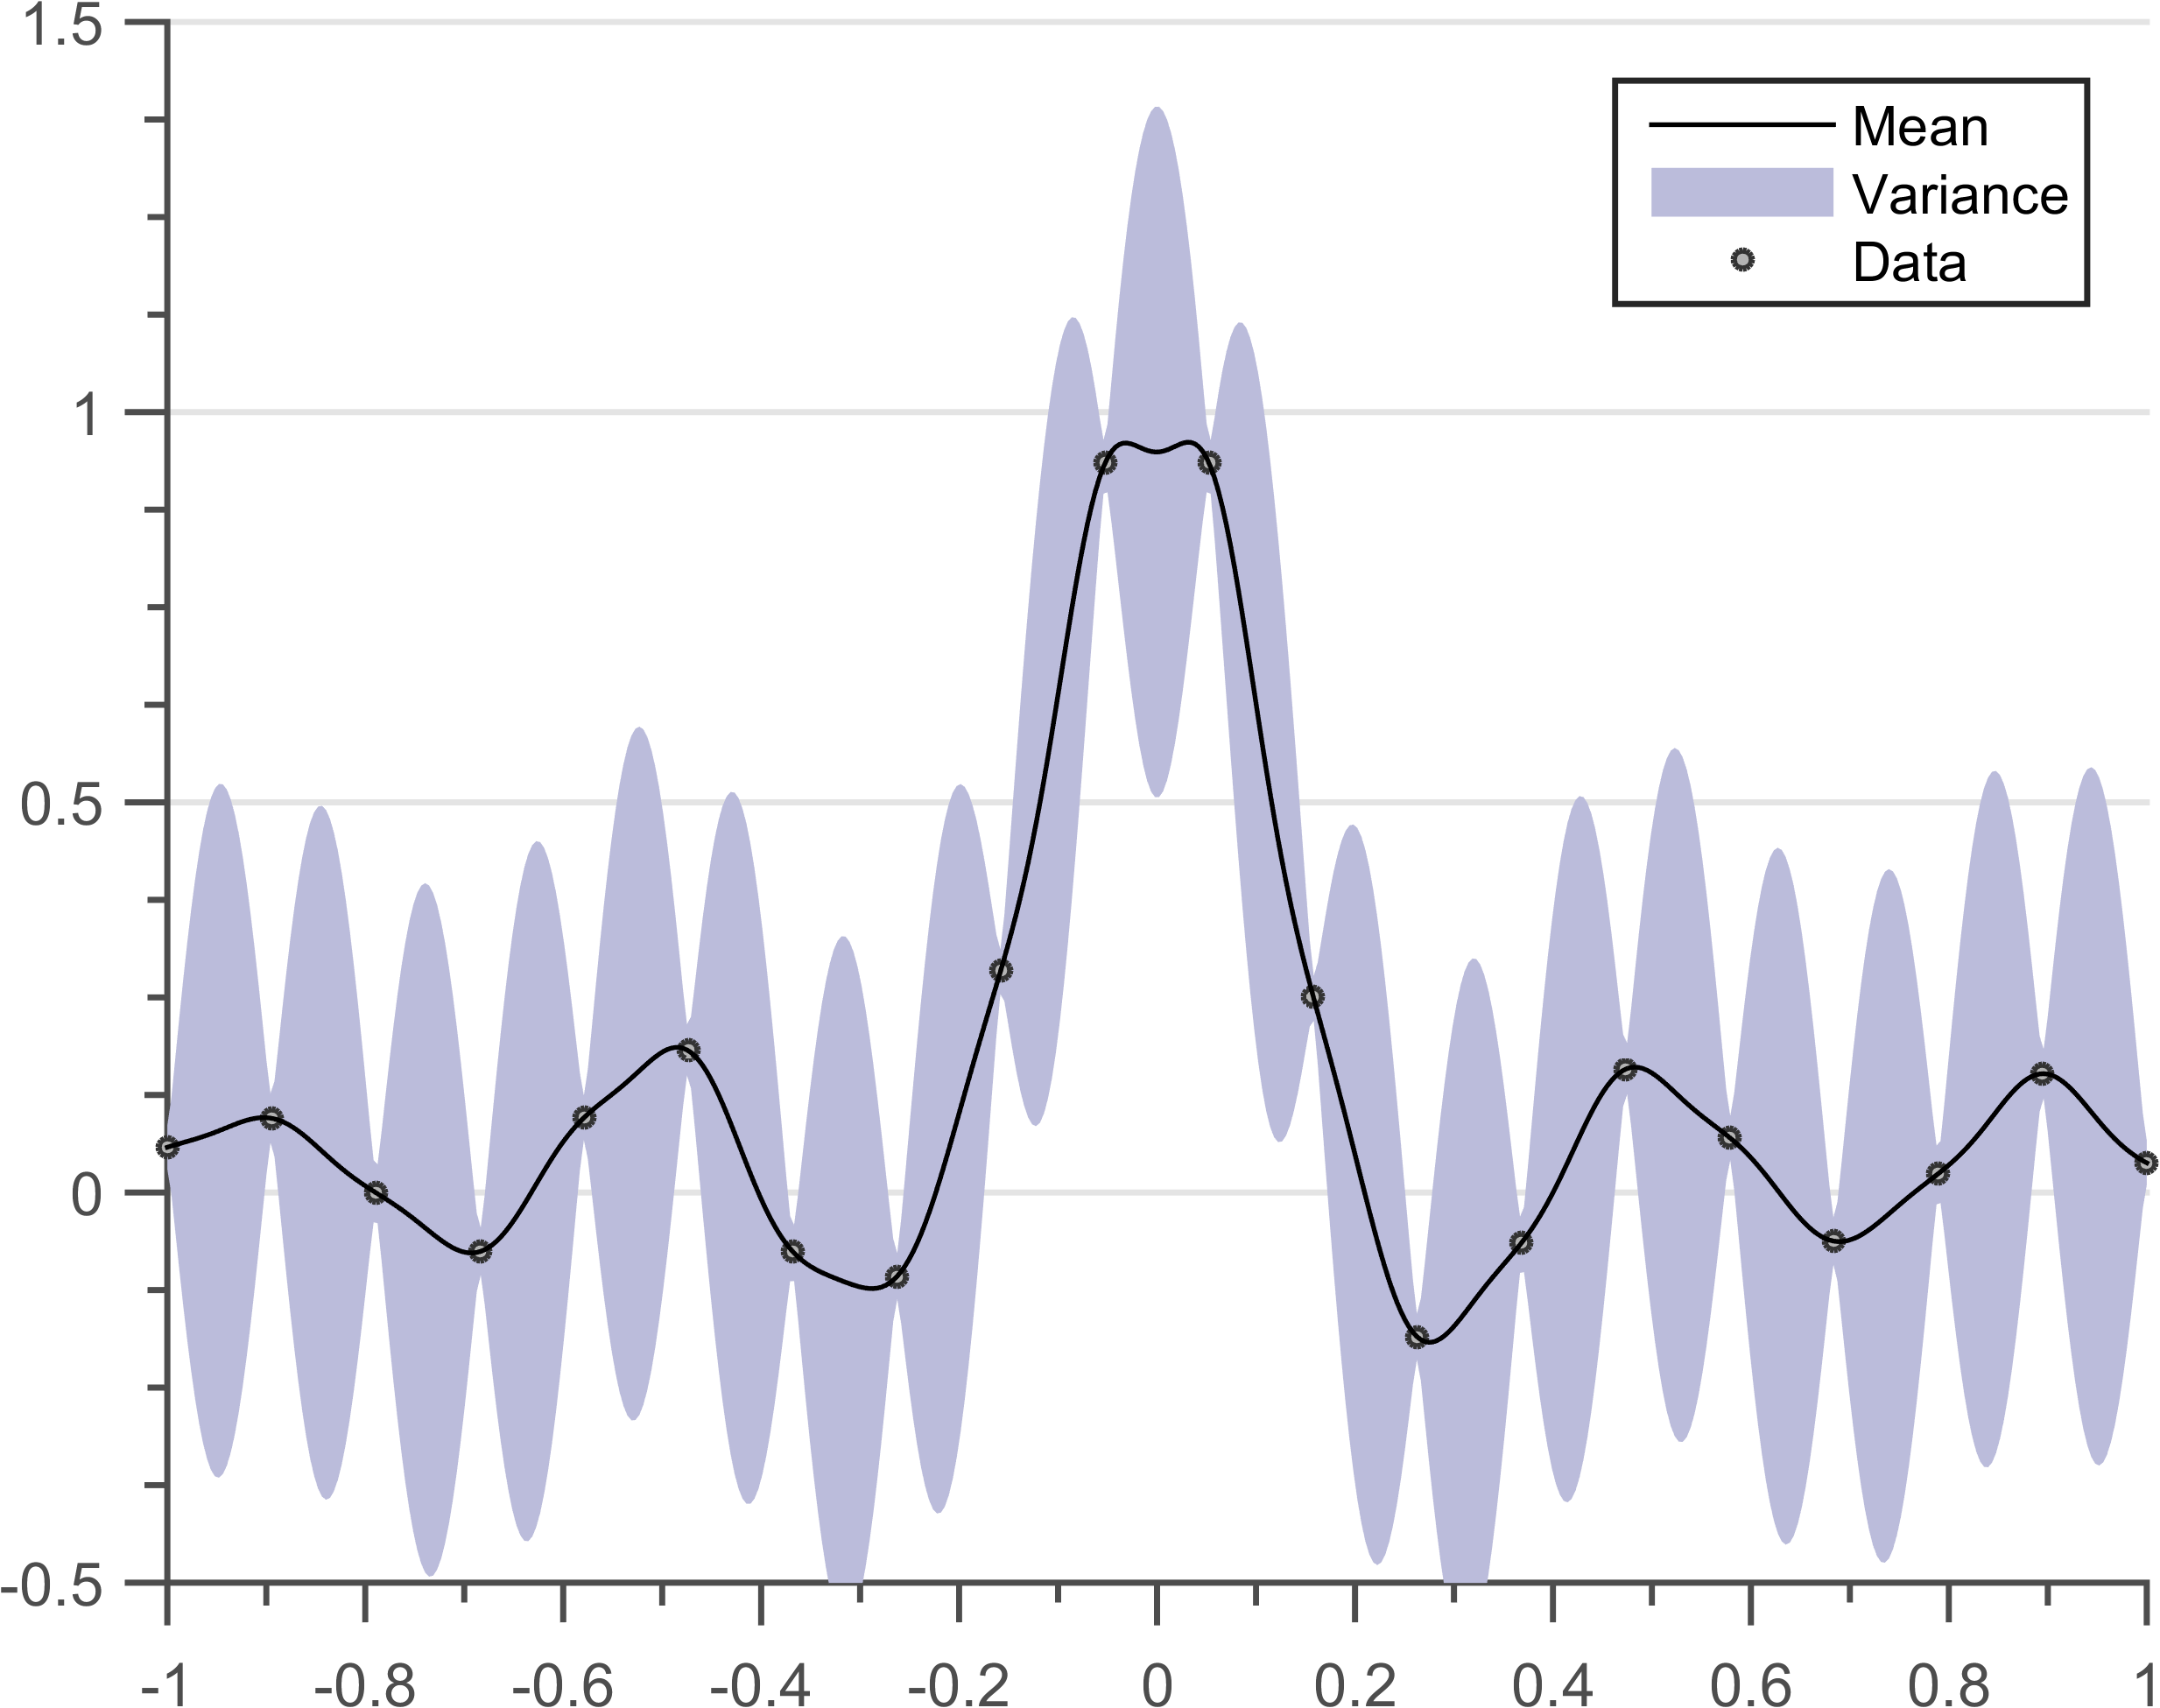
\includegraphics[width=0.45\textwidth]
        {images/posteriorSE1}
        \label{subFigPosterior1}
  }\quad
\subfigure[{Posterior between SE prior with hyper-parameters $(\theta = [0.35, 0.5]; \sigma_{noise} = 0.01)$ and data. }]
%$\log (ML) = -8.2$}]
  {
        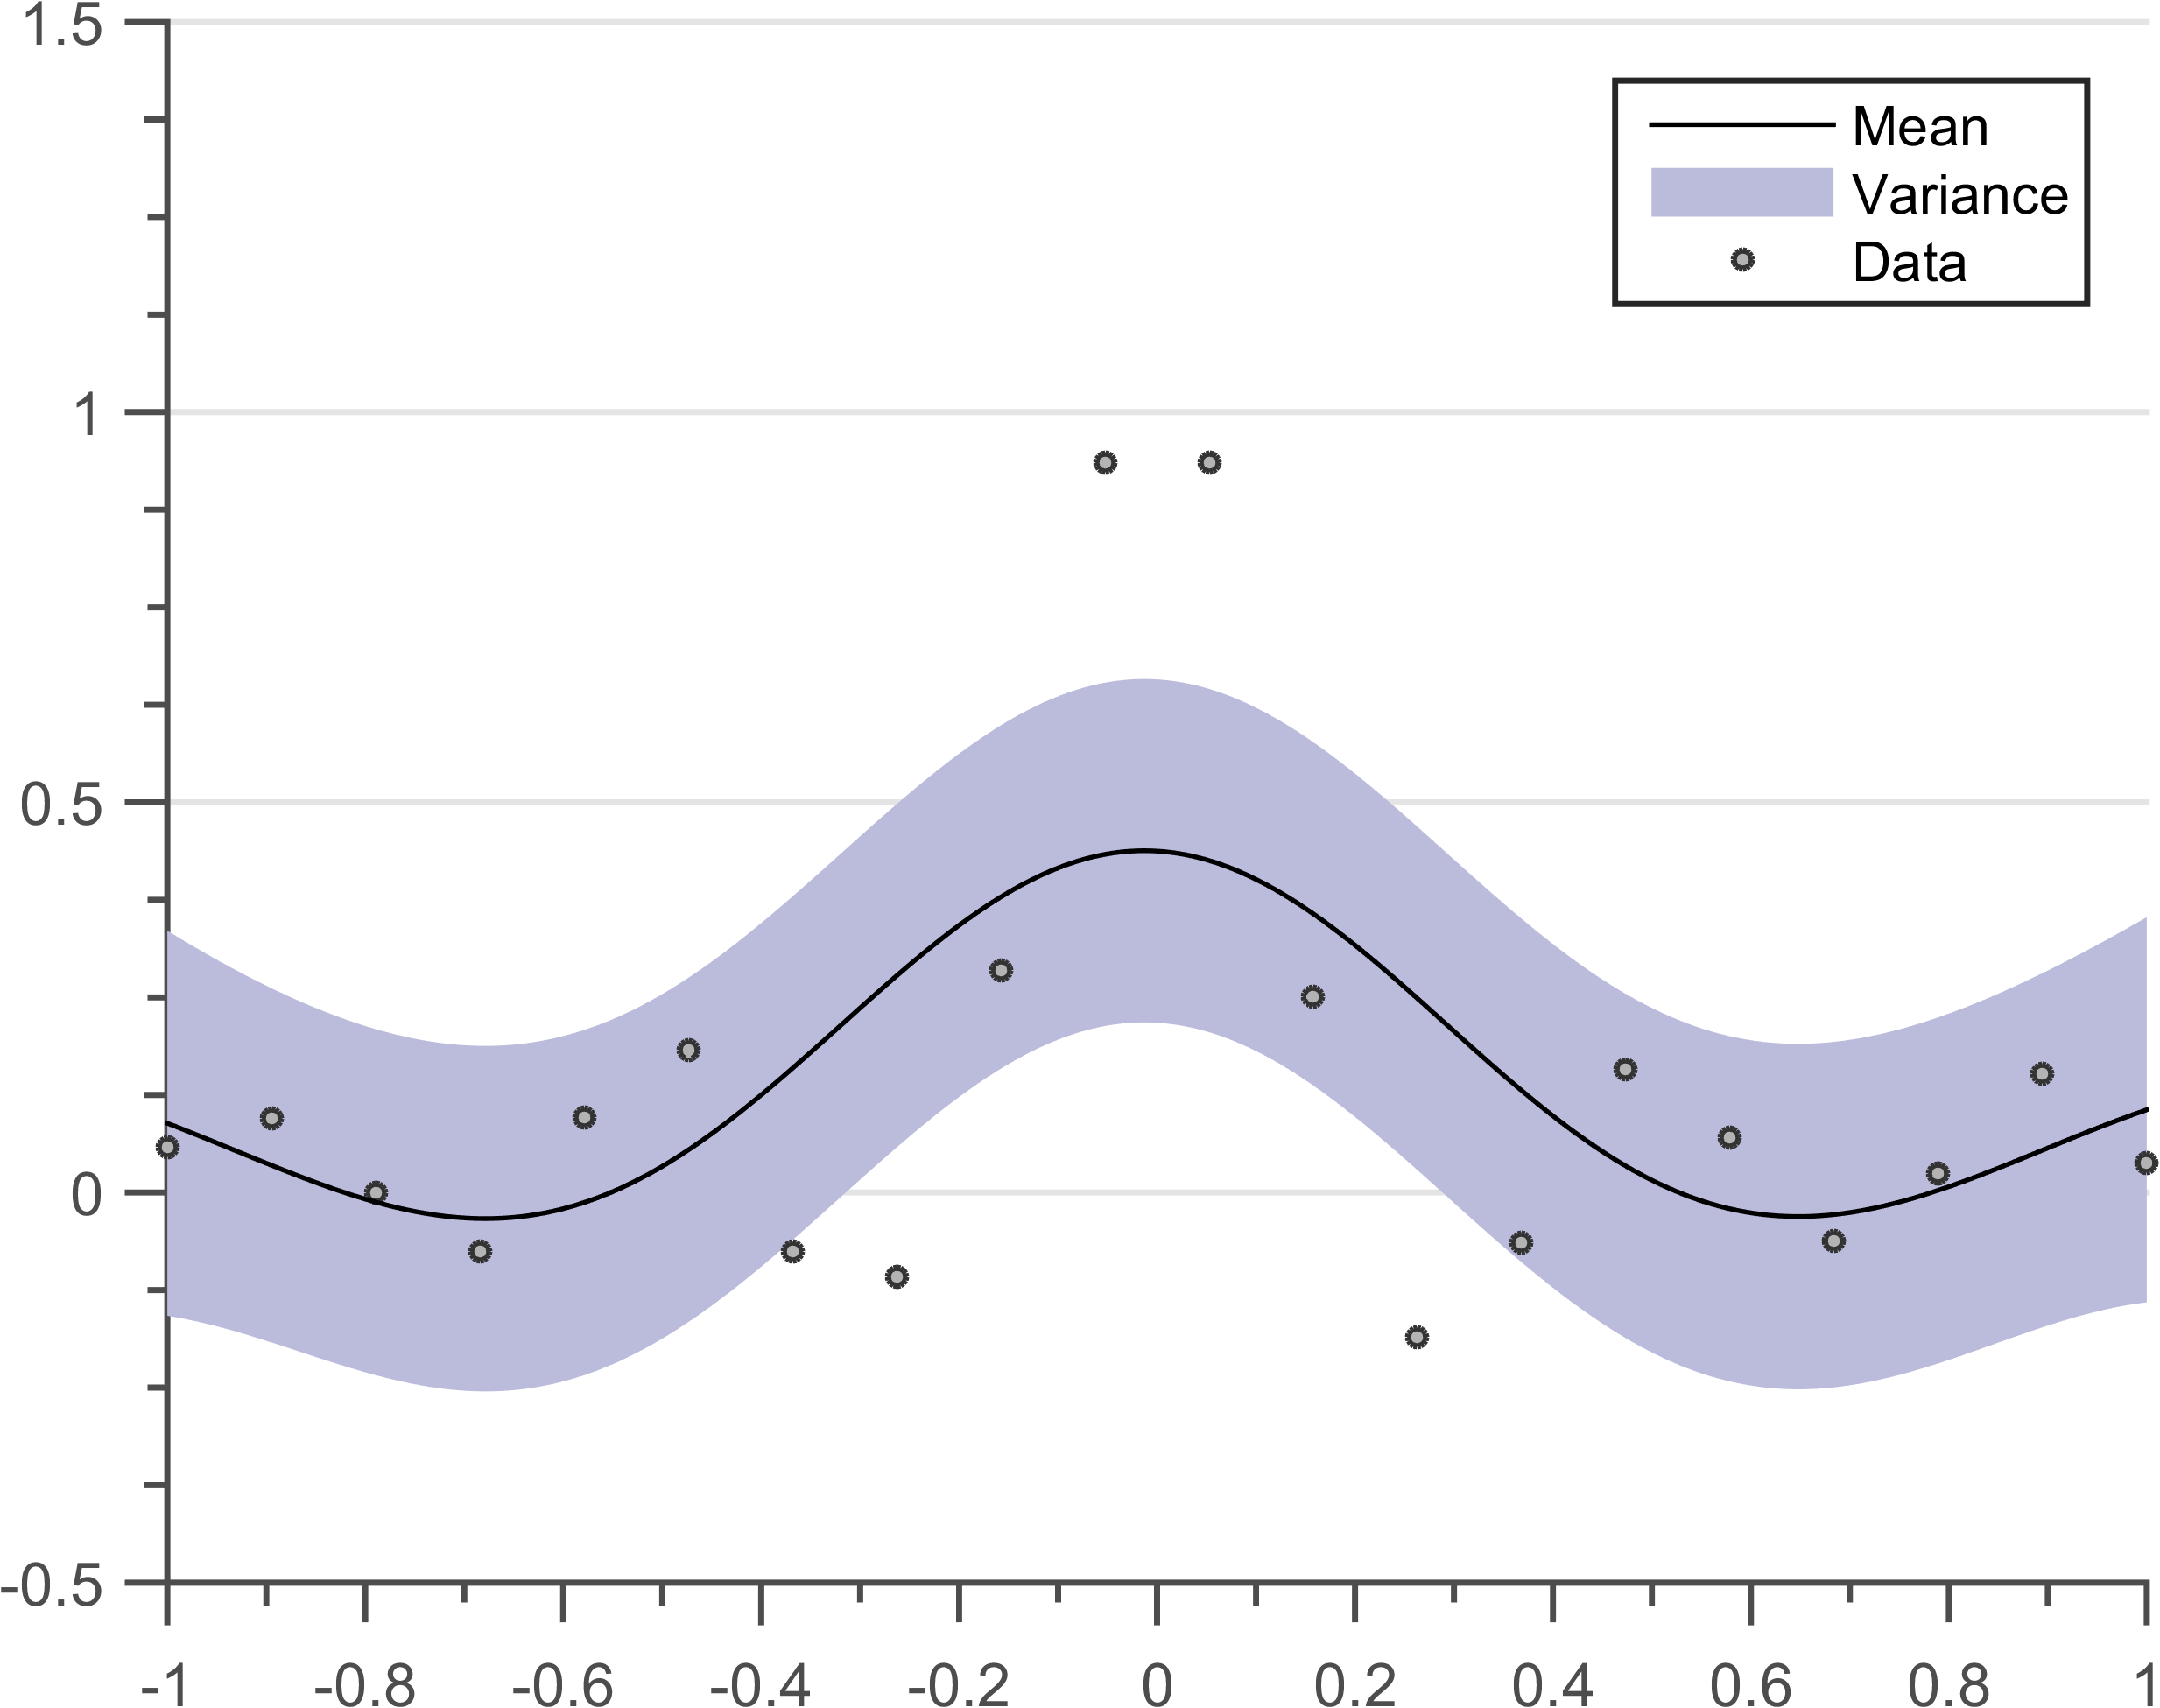
\includegraphics[width=0.45\textwidth]
        {images/posteriorSE3}
        \label{subFigPosterior3}
  }\quad
       \caption{Posteriors for 2 different sets of hyper-parameters. Solid black line defines the mean function, blue region defines 95\% confidence interval (2$\sigma$) distance away from mean. }\label{figGPRMarginal}
\end{figure}

Since hyper-parameters control the family of functions in the hypothesis space and are equivalent to parameters $w$, in a pure Bayesian framework we should put a prior over our hyper-parameters $\Pr[\theta]$ and use Bayes Rule to estimate the posterior $\Pr[\theta \mid \mathcal{D}]$ over our data set. However, this approach becomes intractable and several sampling schemes have been proposed to calculate the posterior of hyper-parameters \cite{osborne2010bayesian, neal2011mcmc}.

Another method to find the optimal hyper-parameters is by performing Cross-Validation (CV). CV procedure is to split the experimental design set into two disjoint sets, one is used for training and the other one is used to monitor the performance
of the surrogate model. A particular case of CV is the Leave-One-Out (LOO) where test sets are obtained by removing one observation at-a-time. Although this can be time-consuming, there are computational short-cuts available for this scheme \cite{rasmussen2006gaussian, dubrule1983cross, le2013multi}. 

In this manuscript we neither put a prior over our hyper-parameters nor use LOO-CV for choosing hyper-parameters. We use the marginal likelihood also called evidence to find optimal hyper-parameters \cite{mackay2003information}. The probability of generating the observations $(Y)$ at the points $(X)$ from a prior (defined by $k(x_{1}, x_{2}, \theta)$) is called the marginal likelihood $\Pr[Y \mid X, \theta]$. In other words, marginal likelihood is the probability that our data set $\mathcal{D}$ was generated from a particular prior. Hence, when we maximize a marginal likelihood we are finding the best prior that could generate our data set. Using equation \ref{equationMeanZeroGPNoisydefinition} and \ref{equationJointPriorNoisy} we get:

\begin{equation}\label{equationMarginalLikelihood}
\begin{aligned}
\Pr[Y(X) \mid X, \theta, \sigma_{n}] & = \mathcal{N}(0 , K(X, X') + \sigma^{2}_{n}I)  \\
& = \frac{1}{\sqrt{(2\pi)^{N/2} K_{XX}}} exp^{-\frac{1}{2}Y^{T}K_{XX}Y}
\end{aligned}
\end{equation}

 Directly, maximizing the marginal likelihood with respect to the hyper-parameters can be inefficient. This is because the marginal likelihood does not vary significantly with the hyper-parameters. Hence to speed up the optimization process we generally maximize the log of marginal likelihood. 

  \begin{equation}\label{eqExactNLML}
\log(\Pr [Y \mid X, \theta ]) = -\frac{1}{2}Y^{T}[K_{XX}+ \sigma_{noise}^{2}I]^{-1}Y - \log\left |  K_{XX}+ \sigma_{noise}^{2}I\right | - \frac{n}{2}\log(2\pi)
  \end{equation}
  
The marginal likelihood is a trade-off between a data-fit term $(\frac{1}{2}Y^{T}K_{XX}^{-1}Y)$ and a model complexity term $(\log\left |  K_{XX}\right |)$. The optimization of ML($\theta$) provides the best compromise in terms of explaining the existing data set \{($x_{i}, y_{i}$)\} and the initial assumptions encoded in the prior. 

Figure \ref{subFigmaximizingMarginalLikelihood} shows the contours of marginal likelihood with respect to length-scale $\theta_{lengthScale}$ and noise $\sigma_{n}$ hyper-parameters. The data set is same as used in figure \ref{figGPRMarginal} and the prior is a zero mean with SE kernel. Figure \ref{subFigPosteriorOptimized} shows the posterior for same data set as used in figure \ref{figGPRMarginal} but for the hyper-parameters where marginal likelihood is maximum. The marginal likelihood could have multiple maximas in the space of hyper-parameters, hence care should be taken while initializing hyper-parameters for optimizing the log of marginal likelihood. 


  \begin{figure}[!ht]
  \centering
    \subfigure[{Marginal likelihood contours for varying noise and length-scale parameter. The amplitude hyper parameter is $(\theta_{amplitude} = [0.35])$.  Also shown on the figure are locations of hyper-parameters for figures \ref{subFigPosterior1} and \ref{subFigPosteriorOptimized}.}]
  {
        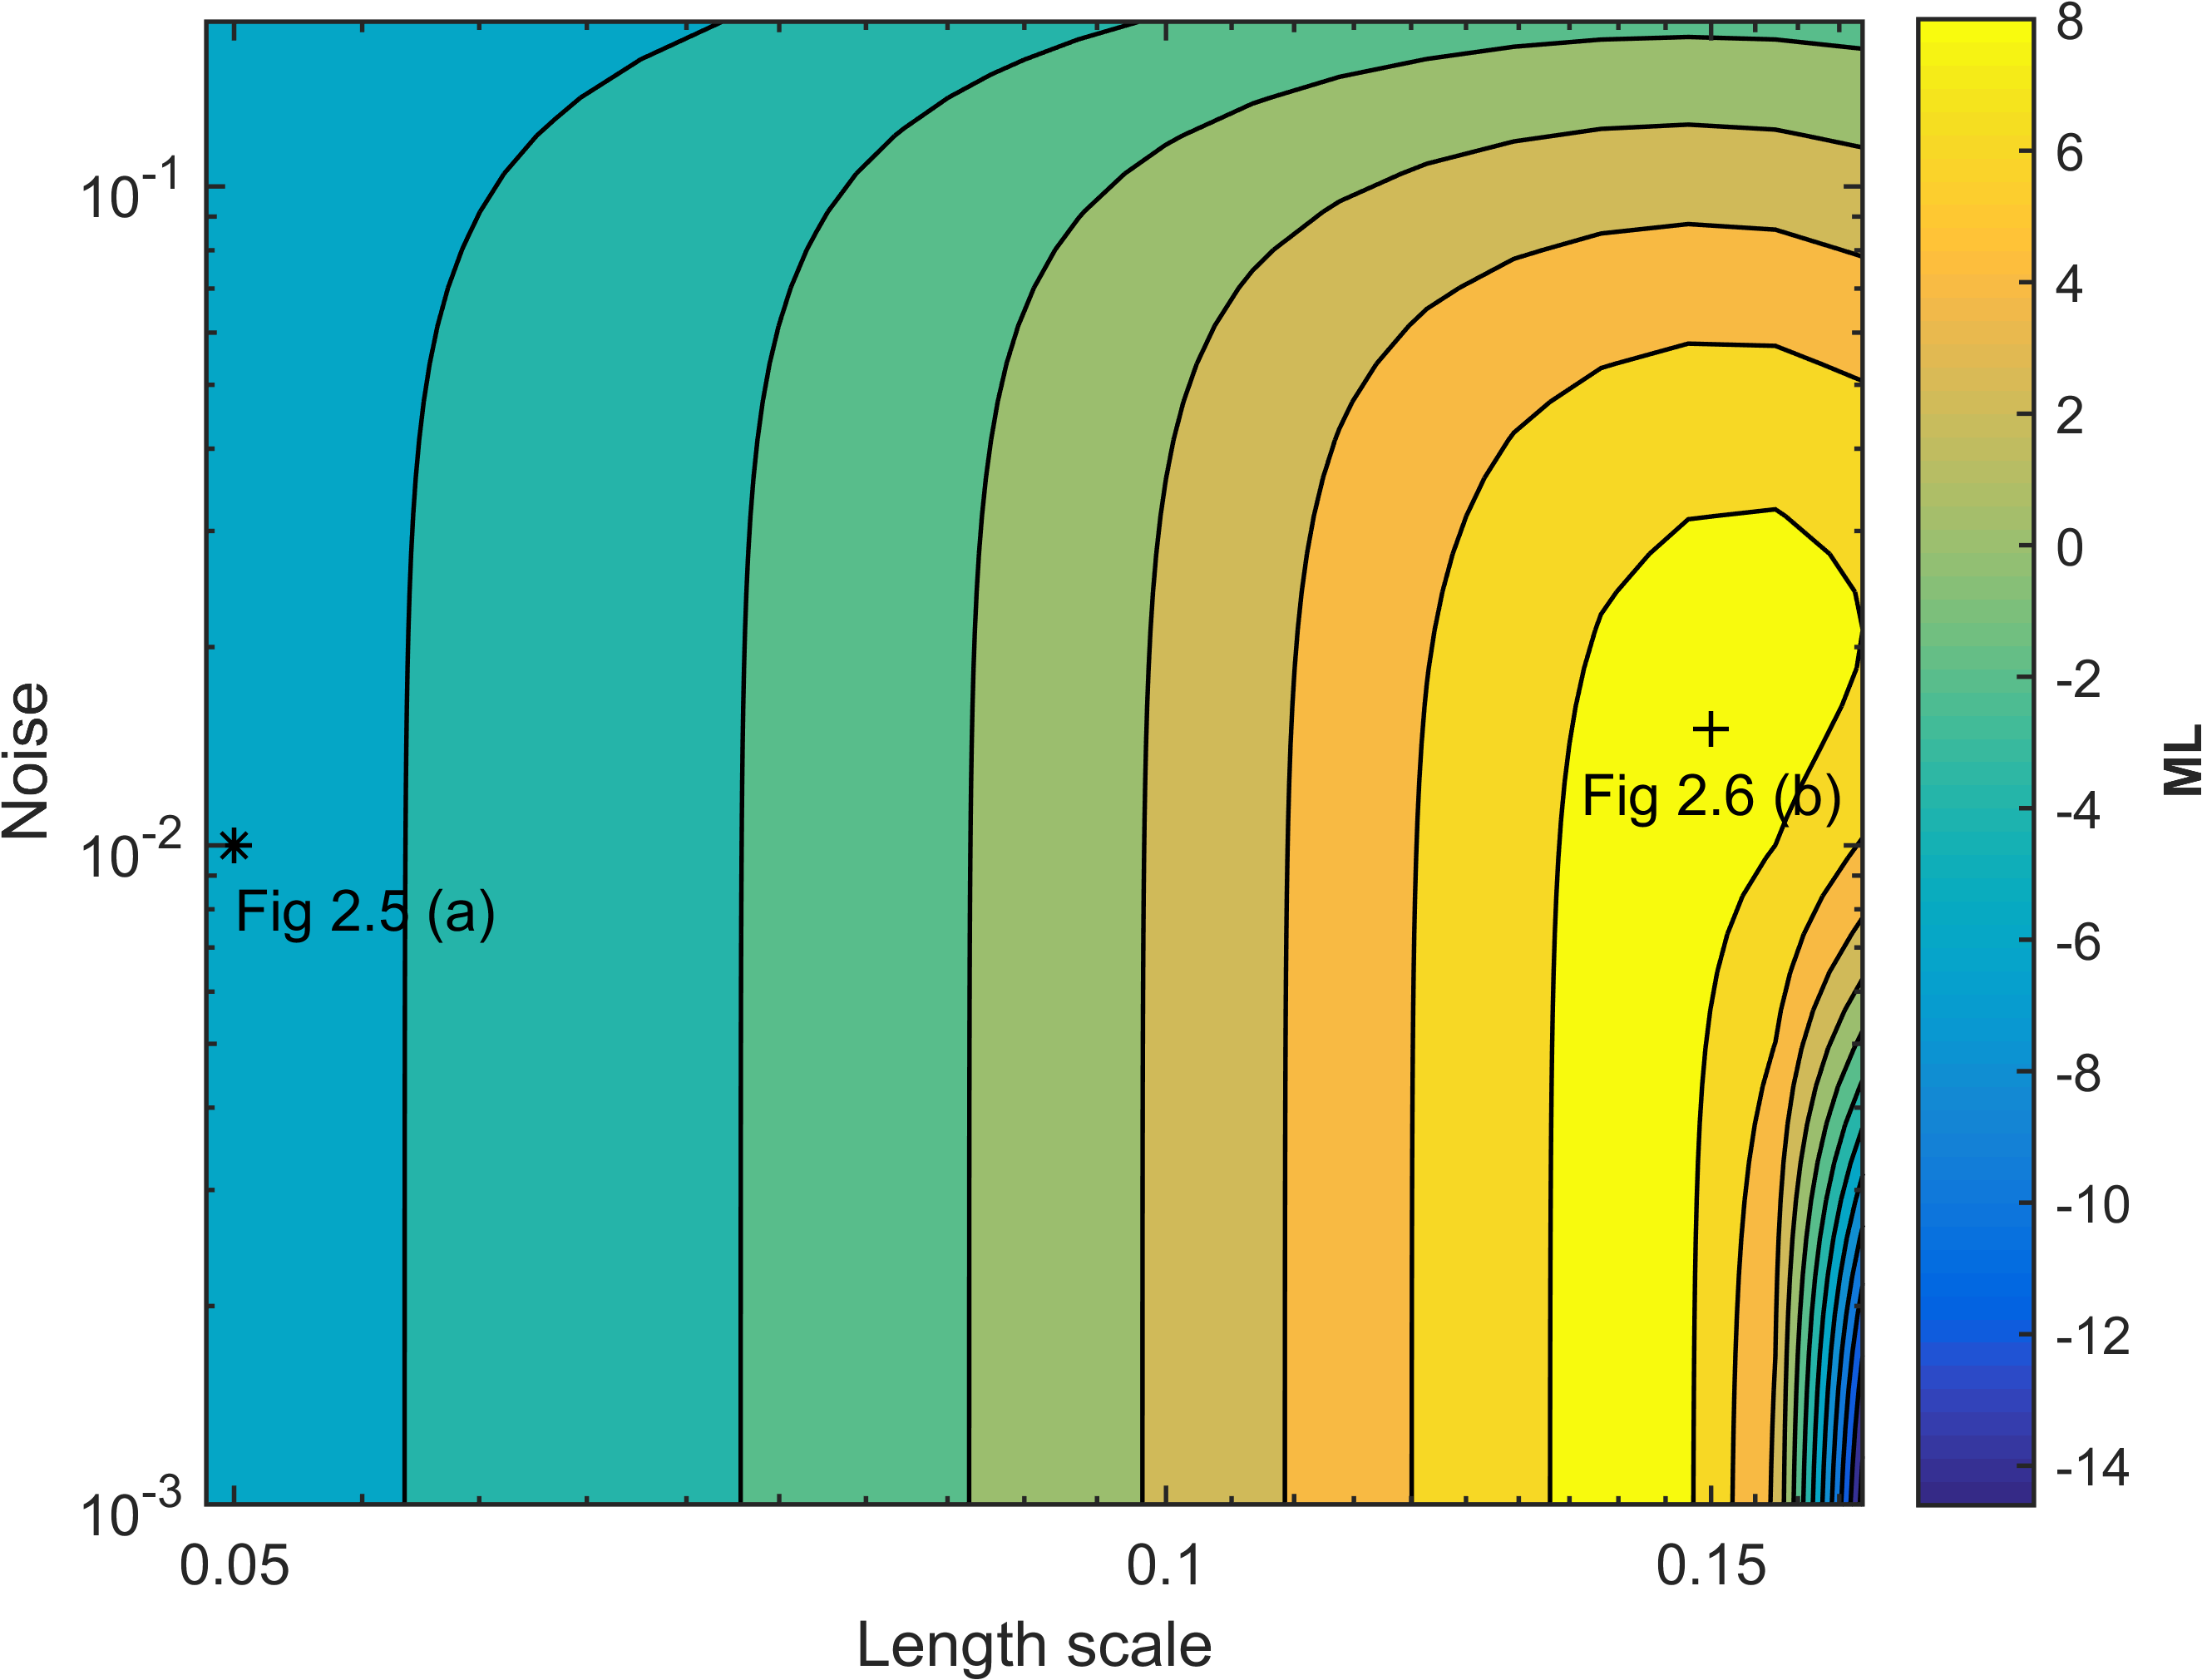
\includegraphics[width=0.45\textwidth]
        {images/maximizingMarginalLikelihood}
        \label{subFigmaximizingMarginalLikelihood}
  }\quad
  \subfigure[{Posterior between SE prior with optimized hyper-parameters $(\theta = [0.35, 0.15]; \sigma_{noise} = 0.015)$ and data. $\log( ML) = 8.04$. Solid black line defines the mean function, blue region defines 95\% confidence interval (2$\sigma$) distance away from mean.}]
  {
        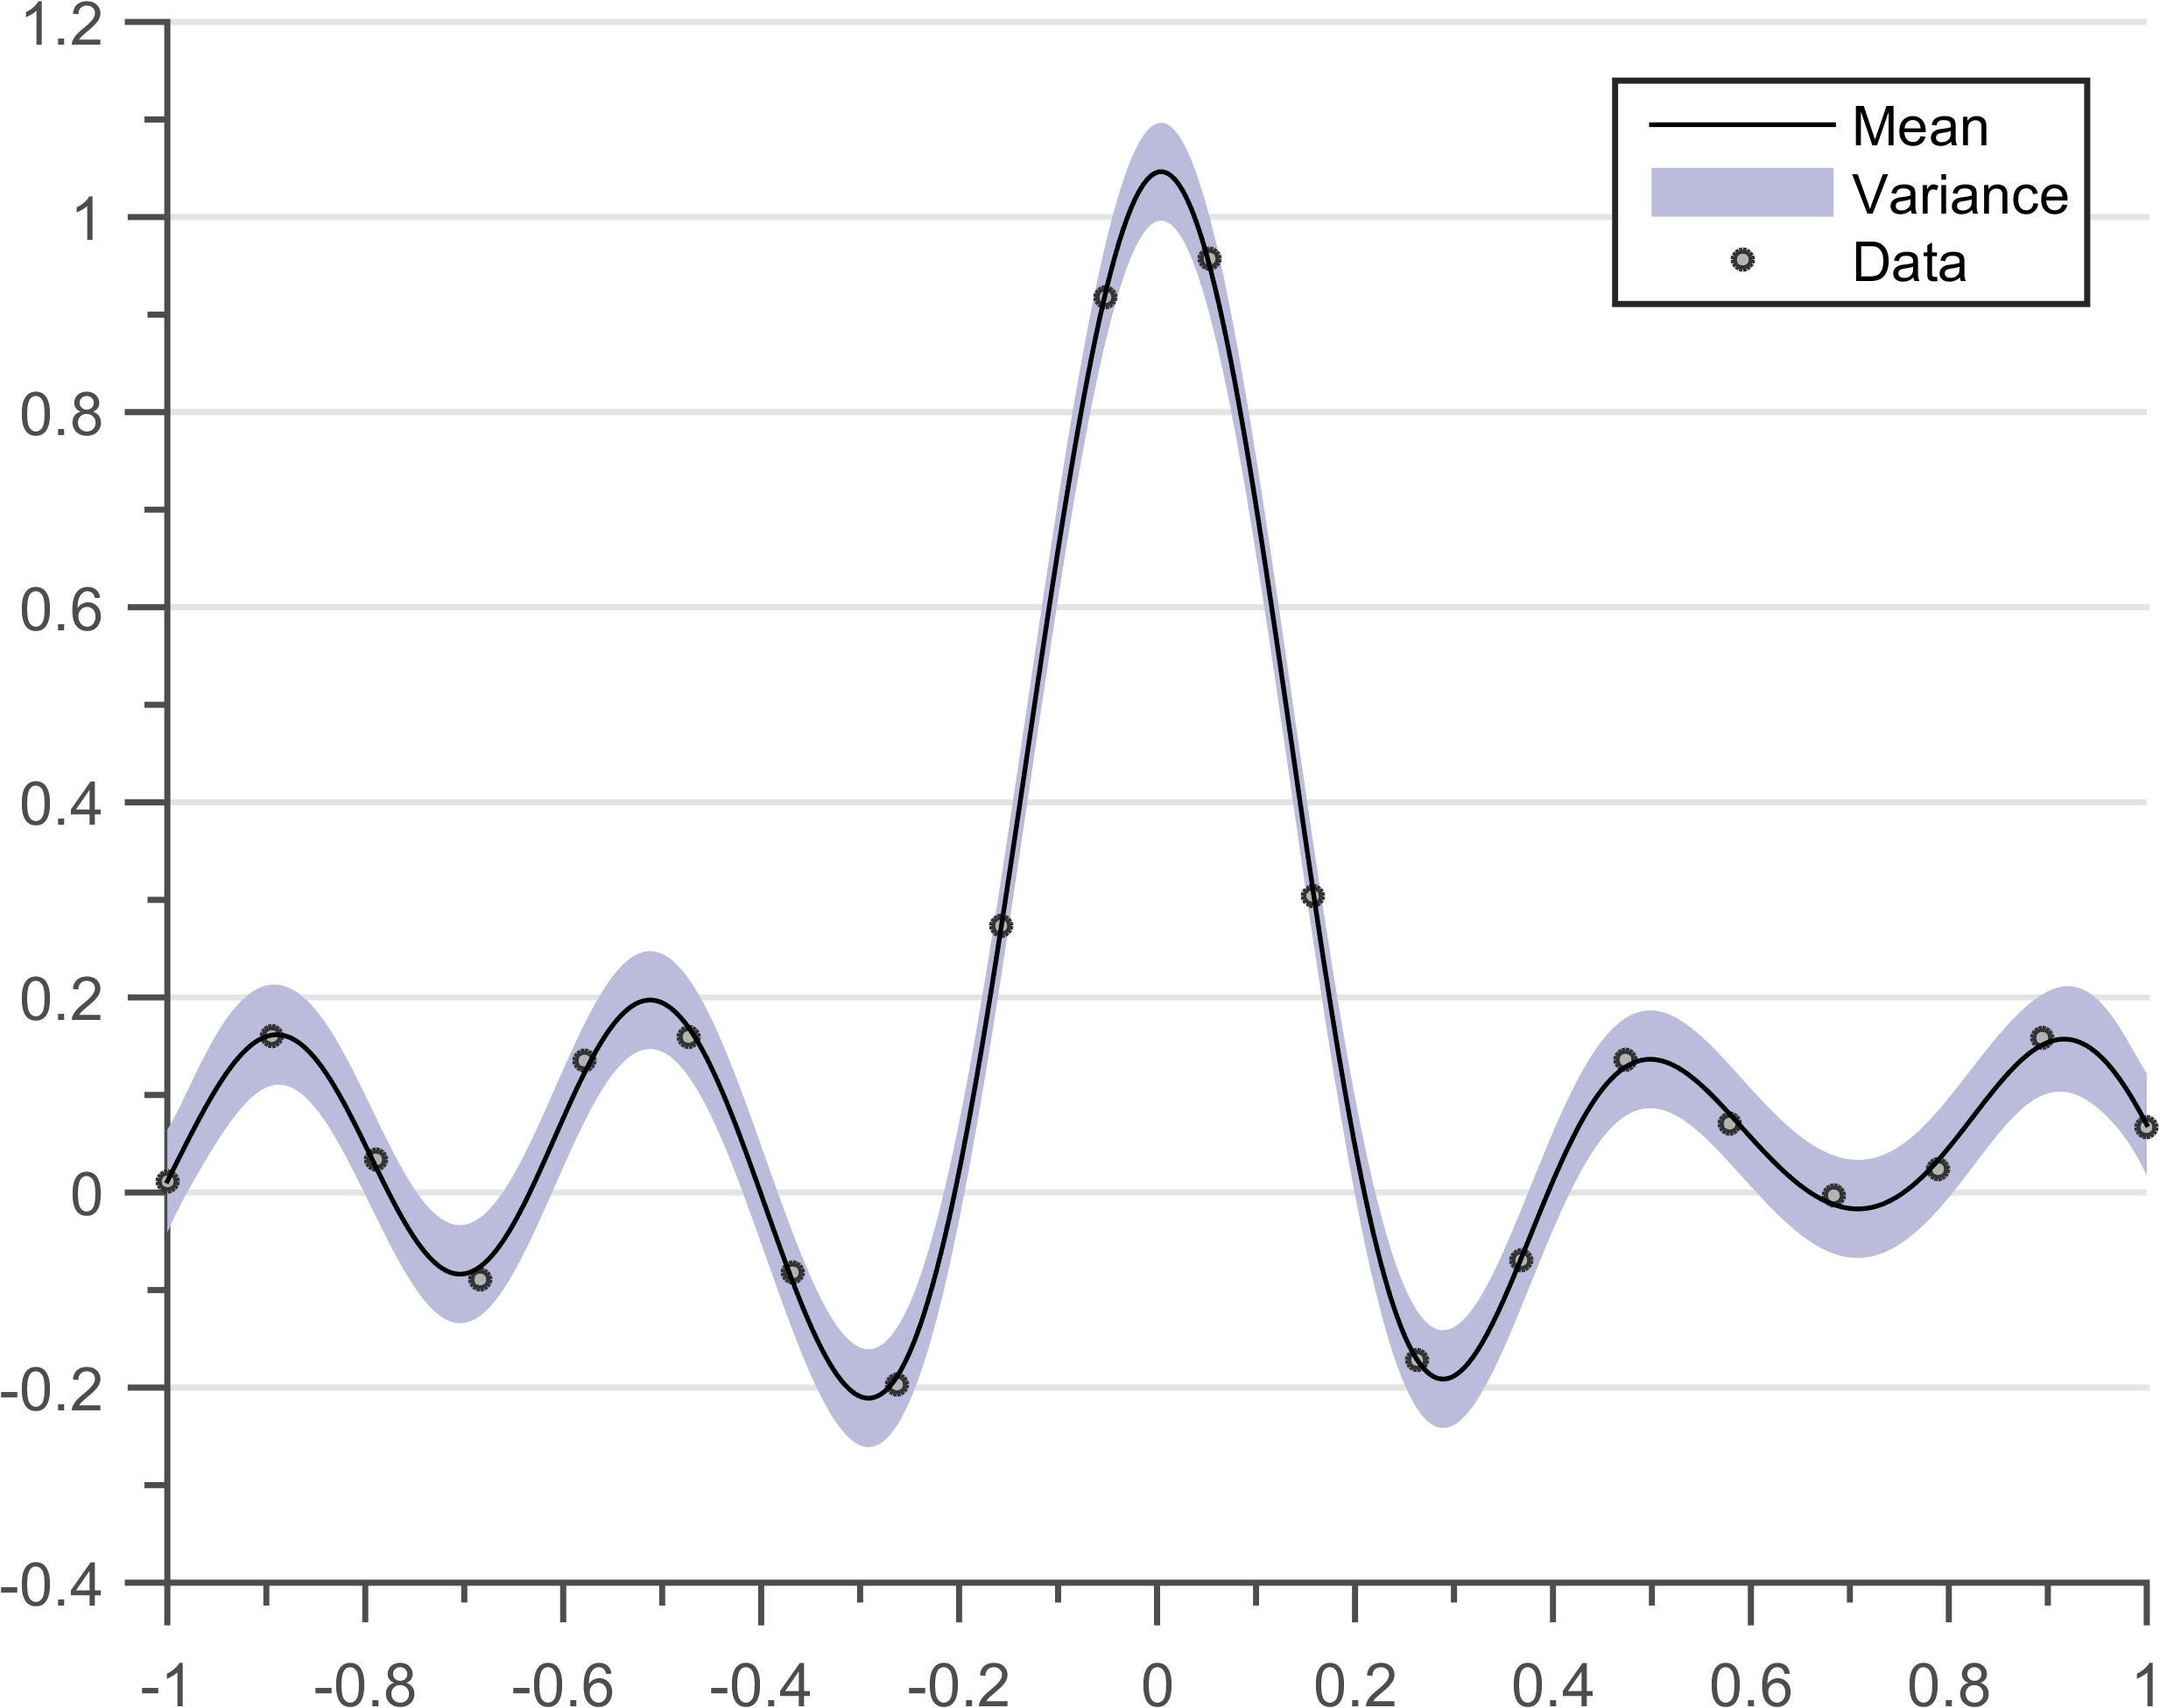
\includegraphics[width=0.45\textwidth]
        {images/posteriorSE}
        \label{subFigPosteriorOptimized}
  }\quad
       \caption{Maximizing marginal likelihood}\label{figGPRMarginalOptimized}
\end{figure}

\section{Discussion}\label{secCH2Discussion}
In this chapter we provide a brief introduction on how to perform Regression with GPs. GPs are the ideal candidate for regression due to their marginalization property, which makes them computationally tractable. Even if GPs define an infinite dimensional random vector, inference on a few points does not require the presence of infinitely other points. This makes drawing functions, calculating posterior distribution and automating selection of hyper-parameters computationally feasible. Thereby making GPs an ideal candidate for defining a Prior distribution in a Bayesian Regression framework. 

The section \ref{secPrior} details the key constituents of a GPs. A GP can be completely parametrized by its mean and covariance function. While, the trend of a GP is defined by its mean function, the structure of its constituent functions is defined by the covariance function. Normally the mean of a GP can be assumed to be zero, since an extra term in the covariance function can represent the mean function. Hence the problem of learning in a GP is exactly the problem of finding suitable properties of the covariance function (subsection \ref{subSecCH2Covariance}). Once a function form of covariance is chosen we can calculate the Gram matrix at desired points and use it to draw random functions from our prior (subsection \ref{subSecSamplingFunctionsGPPrior}). 

The next section \ref{secPosterior} describes how to calculate the posterior distribution. The posterior is the conditional distribution $(\Pr[f(x_{*}) \mid Y, X, \theta])$ for an assumed Prior distribution $(\Pr[f] = GP(0, k(x_{1}, x_{2}, \theta))$ and a set of observed data points $(\mathcal{D} = {X, Y})$. Again, due to the Gaussian assumption the conditional probabilities are all computationally tractable and can be calculated using a few matrix operations, side-stepping the computational burden of performing iterative sampling. Calculating the posterior is easy both in the absence (subsection \ref{subSecPosteriorNoiseFree})and presence (subsection \ref{subSecPosteriorNoisy}) of noise in observations. 

Given a functional form of the covariance, section \ref{secHyperParameter} shows the importance of choosing the correct hyper-parameters. In a pure Bayesian framework the posterior distribution of the hyper-parameters should be calculated ($\Pr[\theta \mid \mathcal{D}]$), but this is computationally intractable needing several iterations for calculation of integrals. A common practice in the community is maximizing the marginal likelihood to automatically choose the hyper-parameters. Marginal likelihood is the probability of a prior distribution $\Pr[f] = GP(0, k(x_{1}, x_{2}, \theta)$ generating the observations $\mathcal{D}$. Hence maximizing the marginal likelihood gives the optimal set of hyper-parameters for a functional form of covariance function (figure \ref{figGPRMarginalOptimized}). 

Calculating the precision matrix $[K_{XX}+ \sigma_{noise}^{2}I]^{-1}$ is an important task in calculating the marginal likelihood (equation \ref{}), posterior mean (equation \ref{}) and covariance (equation \ref{}). Unfortunately, this task has a computational complexity of $\mathcal{O}\left ( N^{3} \right )$ and memory footprint of $\mathcal{O}\left ( N^{2} \right )$. Putting an upper limit of $N \sim 10^4$ on the number of data points, a standard laptop cannot store such a big matrix for inversion \footnote{The computer runs out of memory before we run out of patience :p}. The next chapter describes few methods of performing approximating inference which scales GPs to $N \sim 10^6$ or more data points. 
\chapter{Scaling up Gaussian Process Regression}
\label{chapScalingGPR}

The GP regression approach as mentioned in earlier chapter is intractable for large data sets. For a data set of size \(N\) the covariance matrix \(K_{XX}\) is of size \(N \times N\),  where \(\mathcal{O}\left ( N^{3} \right )\) time is needed for calculating the precision matrix and \(\mathcal{O}\left ( N^{2} \right )\) memory for storage. Since, inverting the covariance matrix takes considerable amount of time and memory, almost all techniques to scale up GP regression try to approximate the inversion of Gram matrix \(K_{XX}\). 

Let us take the example of an SE kernel, for a large value of length-scale the Gram matrix (\(K_{XX}\)) is spread out and has a rank lower than  \(N\) (figure \ref{subFigSEPrior_2}). Due to this low-rank characteristic the Gram matrix can be approximated as a lower rank form reducing the cost of inverting the Gram matrix. In the GP literature sparse approximations (section \ref{secSparseApprox}) use a set of inducing points to compress the information of the several observations through the low-rank approximation. 

For the same SE kernel if the length-scale tends to a low value the Gram matrix is not of low-rank but tends to a diagonal matrix (figure \ref{subFigSEPrior_1}). In the GP literature the mixture of experts (section \ref{secDgp}) methodology exploits the block diagonal nature of the Gram matrix by distributing data points into a subset of experts, assuming independence across experts and distributing the calculations into several batches. The first regime suggests global (numerical) low-rank approximations while the second regime suggests local block-diagonal approximations \cite{march2015askit, chenhan2016inv}. 

The remaining chapter unfolds as follows, section \ref{secSparseApprox} describes the Sparse Approximations detailing several methods of choosing inducing points and then performing experiments on a toy dataset. Section \ref{secDgp} describes the Distributed GP methodology detailing several methods for merging of experts and then performing experiments on the same toy-dataset. 

\section{Sparse Approximations}\label{secSparseApprox}
Sparse methods use a small subset of input points as support or inducing points to approximate the Gram matrix. Suppose we use \(M\) inducing points \(X^{m} = \{x^{m}_{1}; x^{m}_{2}; \ldots; x^{m}_{M}\}\), such that \(M < N\). The points \(X^{m}\) can be a subset of training inputs in the input space. 


\subsection{Nystr\"{o}m Approximation}\label{subSecNystrom} 

Using Nystr\"{o}m approximation the Gram matrix can be approximated as equation \ref{eqnSparseNystormGram} \textbf{add more detail here as well}. Refer to \cite{quinonero2005unifying, seeger2003fast} for more detail. 

\begin{equation}\label{eqnSparseNystormGram}
K_{nystorm}(X, X) = K(X, X^{m})K(X^{m}, X^{m})^{-1}K(X^{m}, X)
\end{equation}

Here, \(K(X^{m}, X^{m})\) is a \(M \times M\) Gram matrix evaluated at inducing points \(X^{m}\), \(K(X, X^{m})\) is an \(N \times M\) Gram matrix between training points and inducing points. The inversion of approximate matrix takes \(\mathcal{O}\left ( NM^{2} \right )\) time to compute. Figure \ref{subFigNystormSEmatrix} is an approximate Gram matrix using Nystr\"{o}m approximation of the matrix in figure \ref{subFigcovSEmatrix_1} at the input points \(X^{*} = \{[0:0.02:1]\}\). The inducing points \(X^{m}\) were chosen randomly from the set of input points and their location is denoted by white lines. We can observe that if the gap between inducing points increases then accuracy of Gram matrix degrades (eg. at \(x \sim 0.5\)). Figure \ref{subFignystormSEmatrixUniform} is again an approximated Gram matrix using Nystr\"{o}m approximation of the matrix in figure \ref{subFigcovSEmatrix_1}. This time the equally spaced inducing points are chosen in the range of \(X^{*}\). Notice the significant improvement in the Gram matrix upon different set of inducing inputs.

\begin{figure}[!ht]
  \centering
    \subfigure[{Approximated Gram matrix using Nystr\"{o}m approximation for a Standard Exponential (SE) Kernel with \((\theta = [1, 0.2])\) (figure \ref{subFigcovSEmatrix_1}) at the input points \(X^{*} = \{[0:0.02:1]\}\). The inducing points were chosen randomly, the white lines denote the location of inducing points. }]
  {
        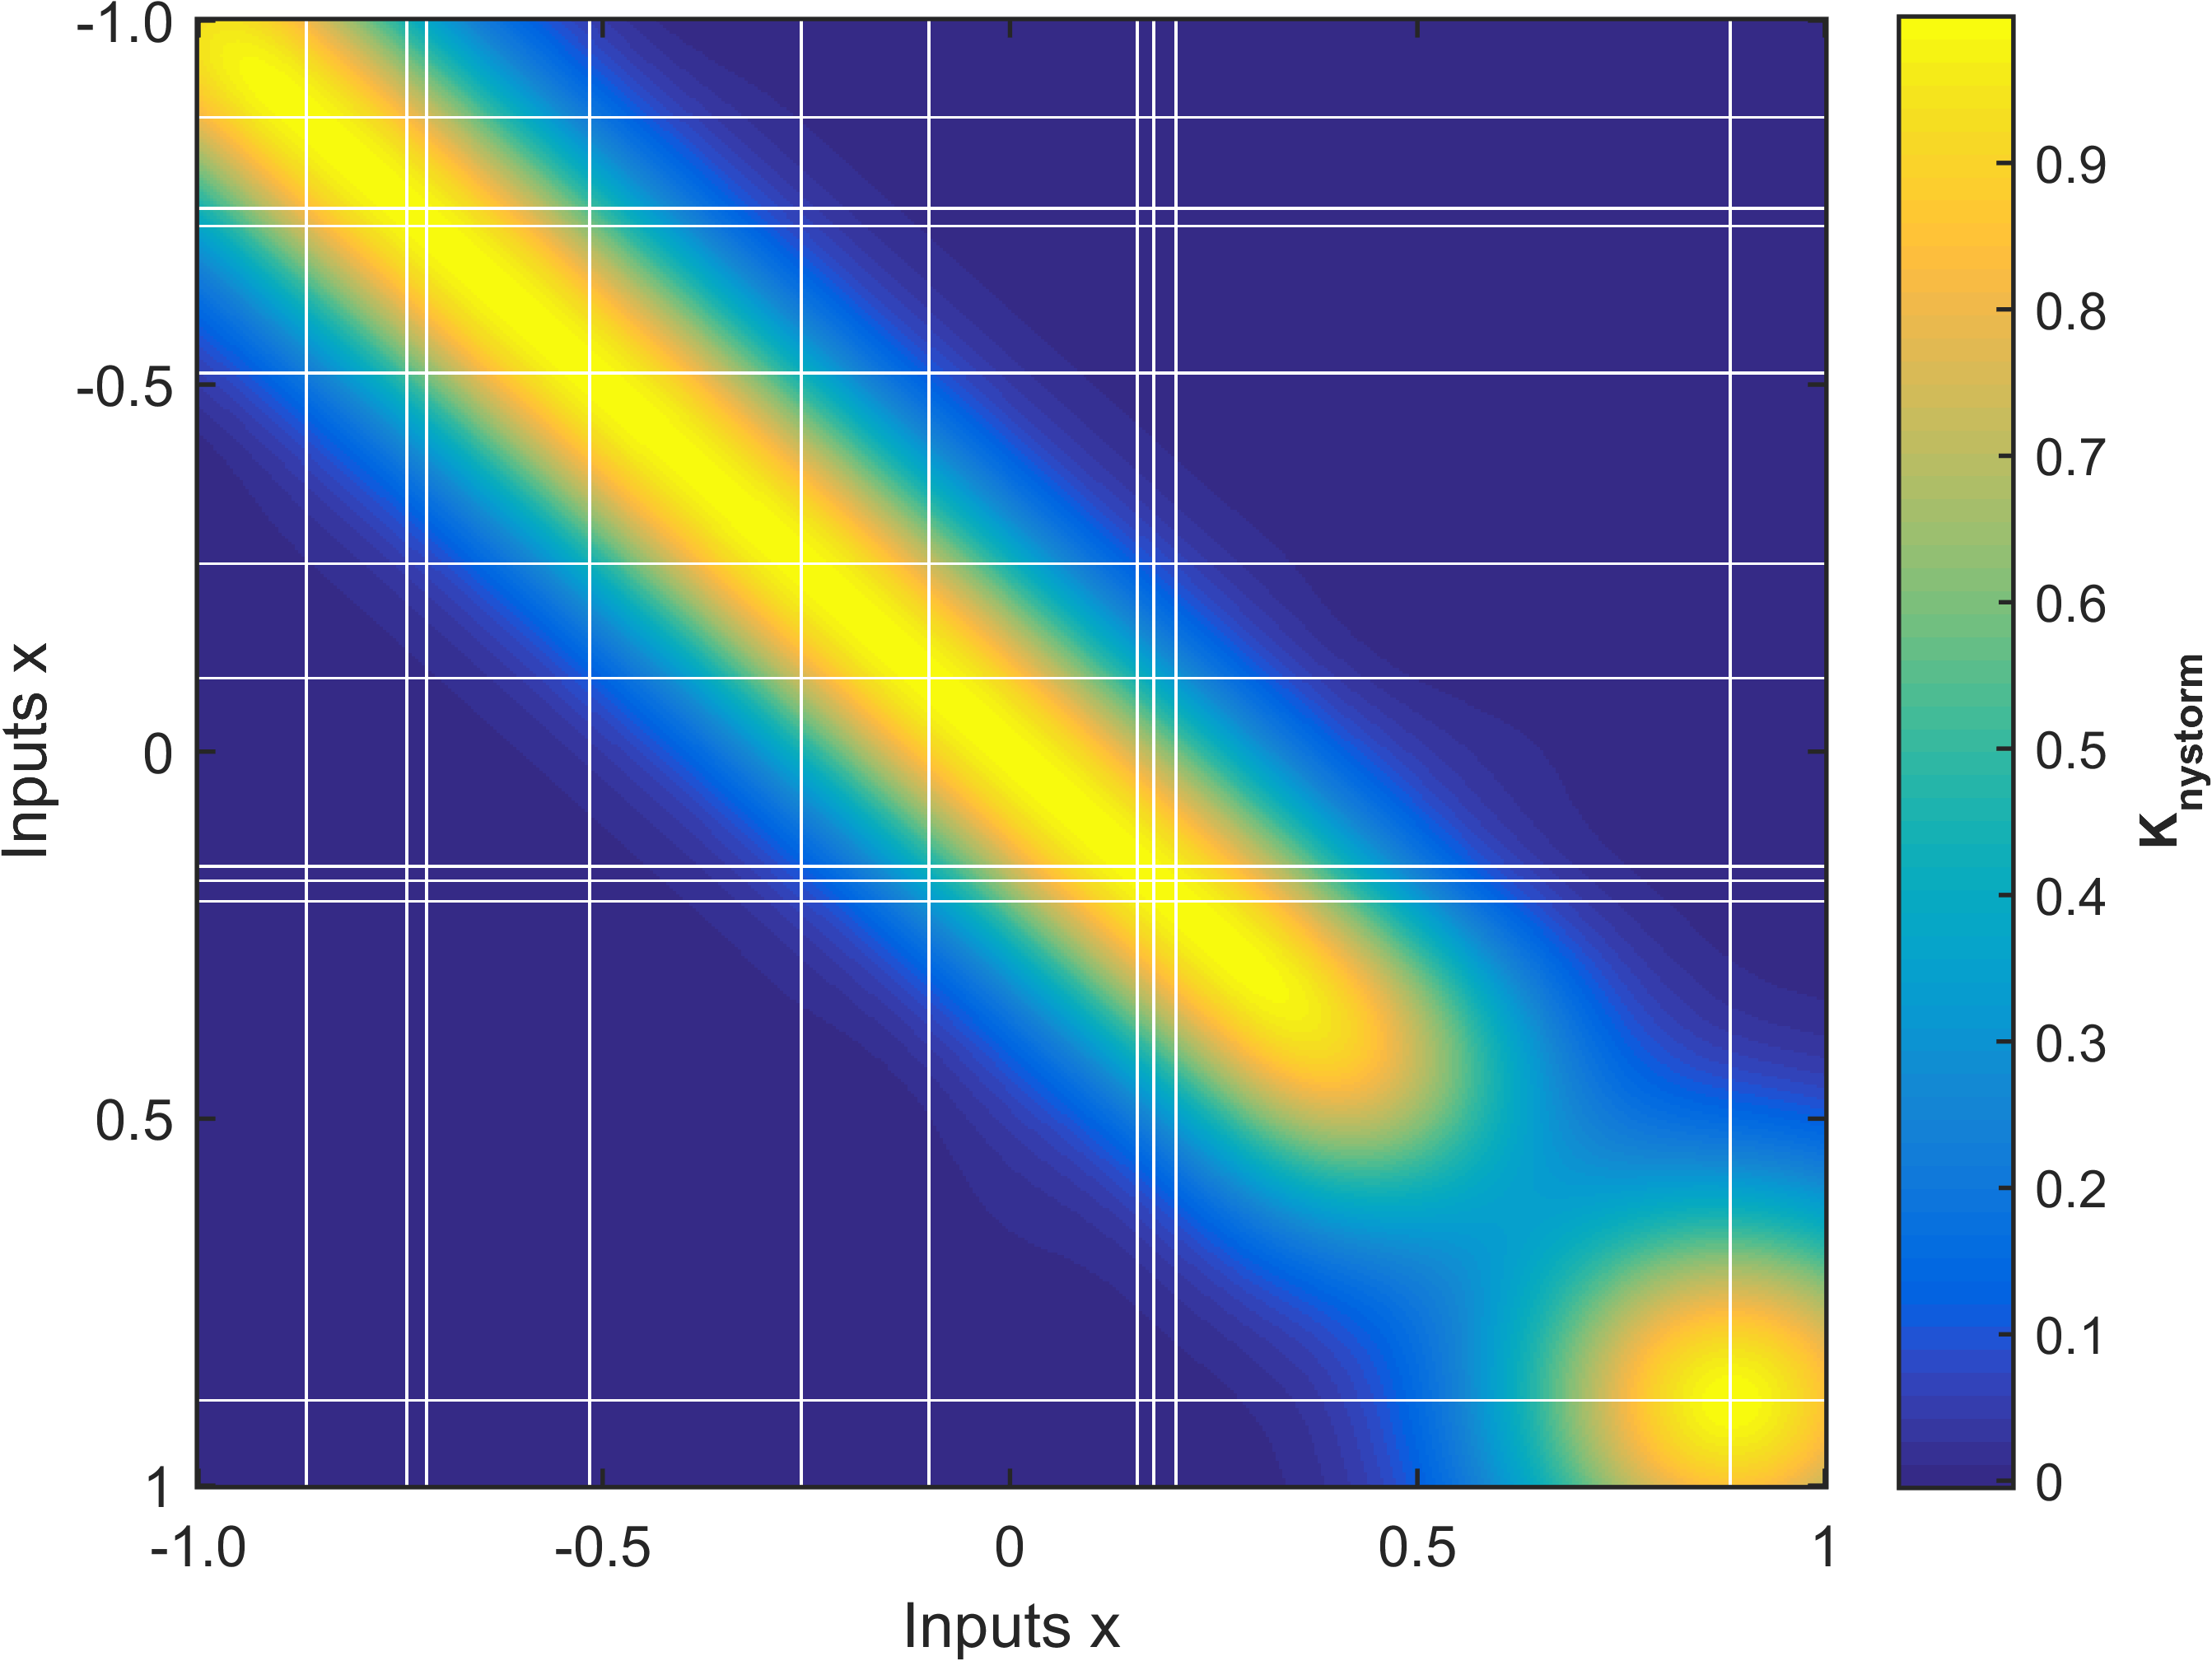
\includegraphics[width=0.45\textwidth]
        {images/nystormSEmatrix}
        \label{subFigNystormSEmatrix}
  }\quad
\subfigure[{Approximated Gram matrix using Nystr\"{o}m approximation for a Standard Exponential (SE) Kernel with \((\theta = [1, 0.2])\) (figure \ref{subFigcovSEmatrix_1}) at the input points \(X^{*} = \{[0:0.02:1]\}\). The white lines denote the location of inducing points, the inducing points are uniformly distributed. Notice the significant improvement in Gram matrix due to different inducing inputs}]
  {
        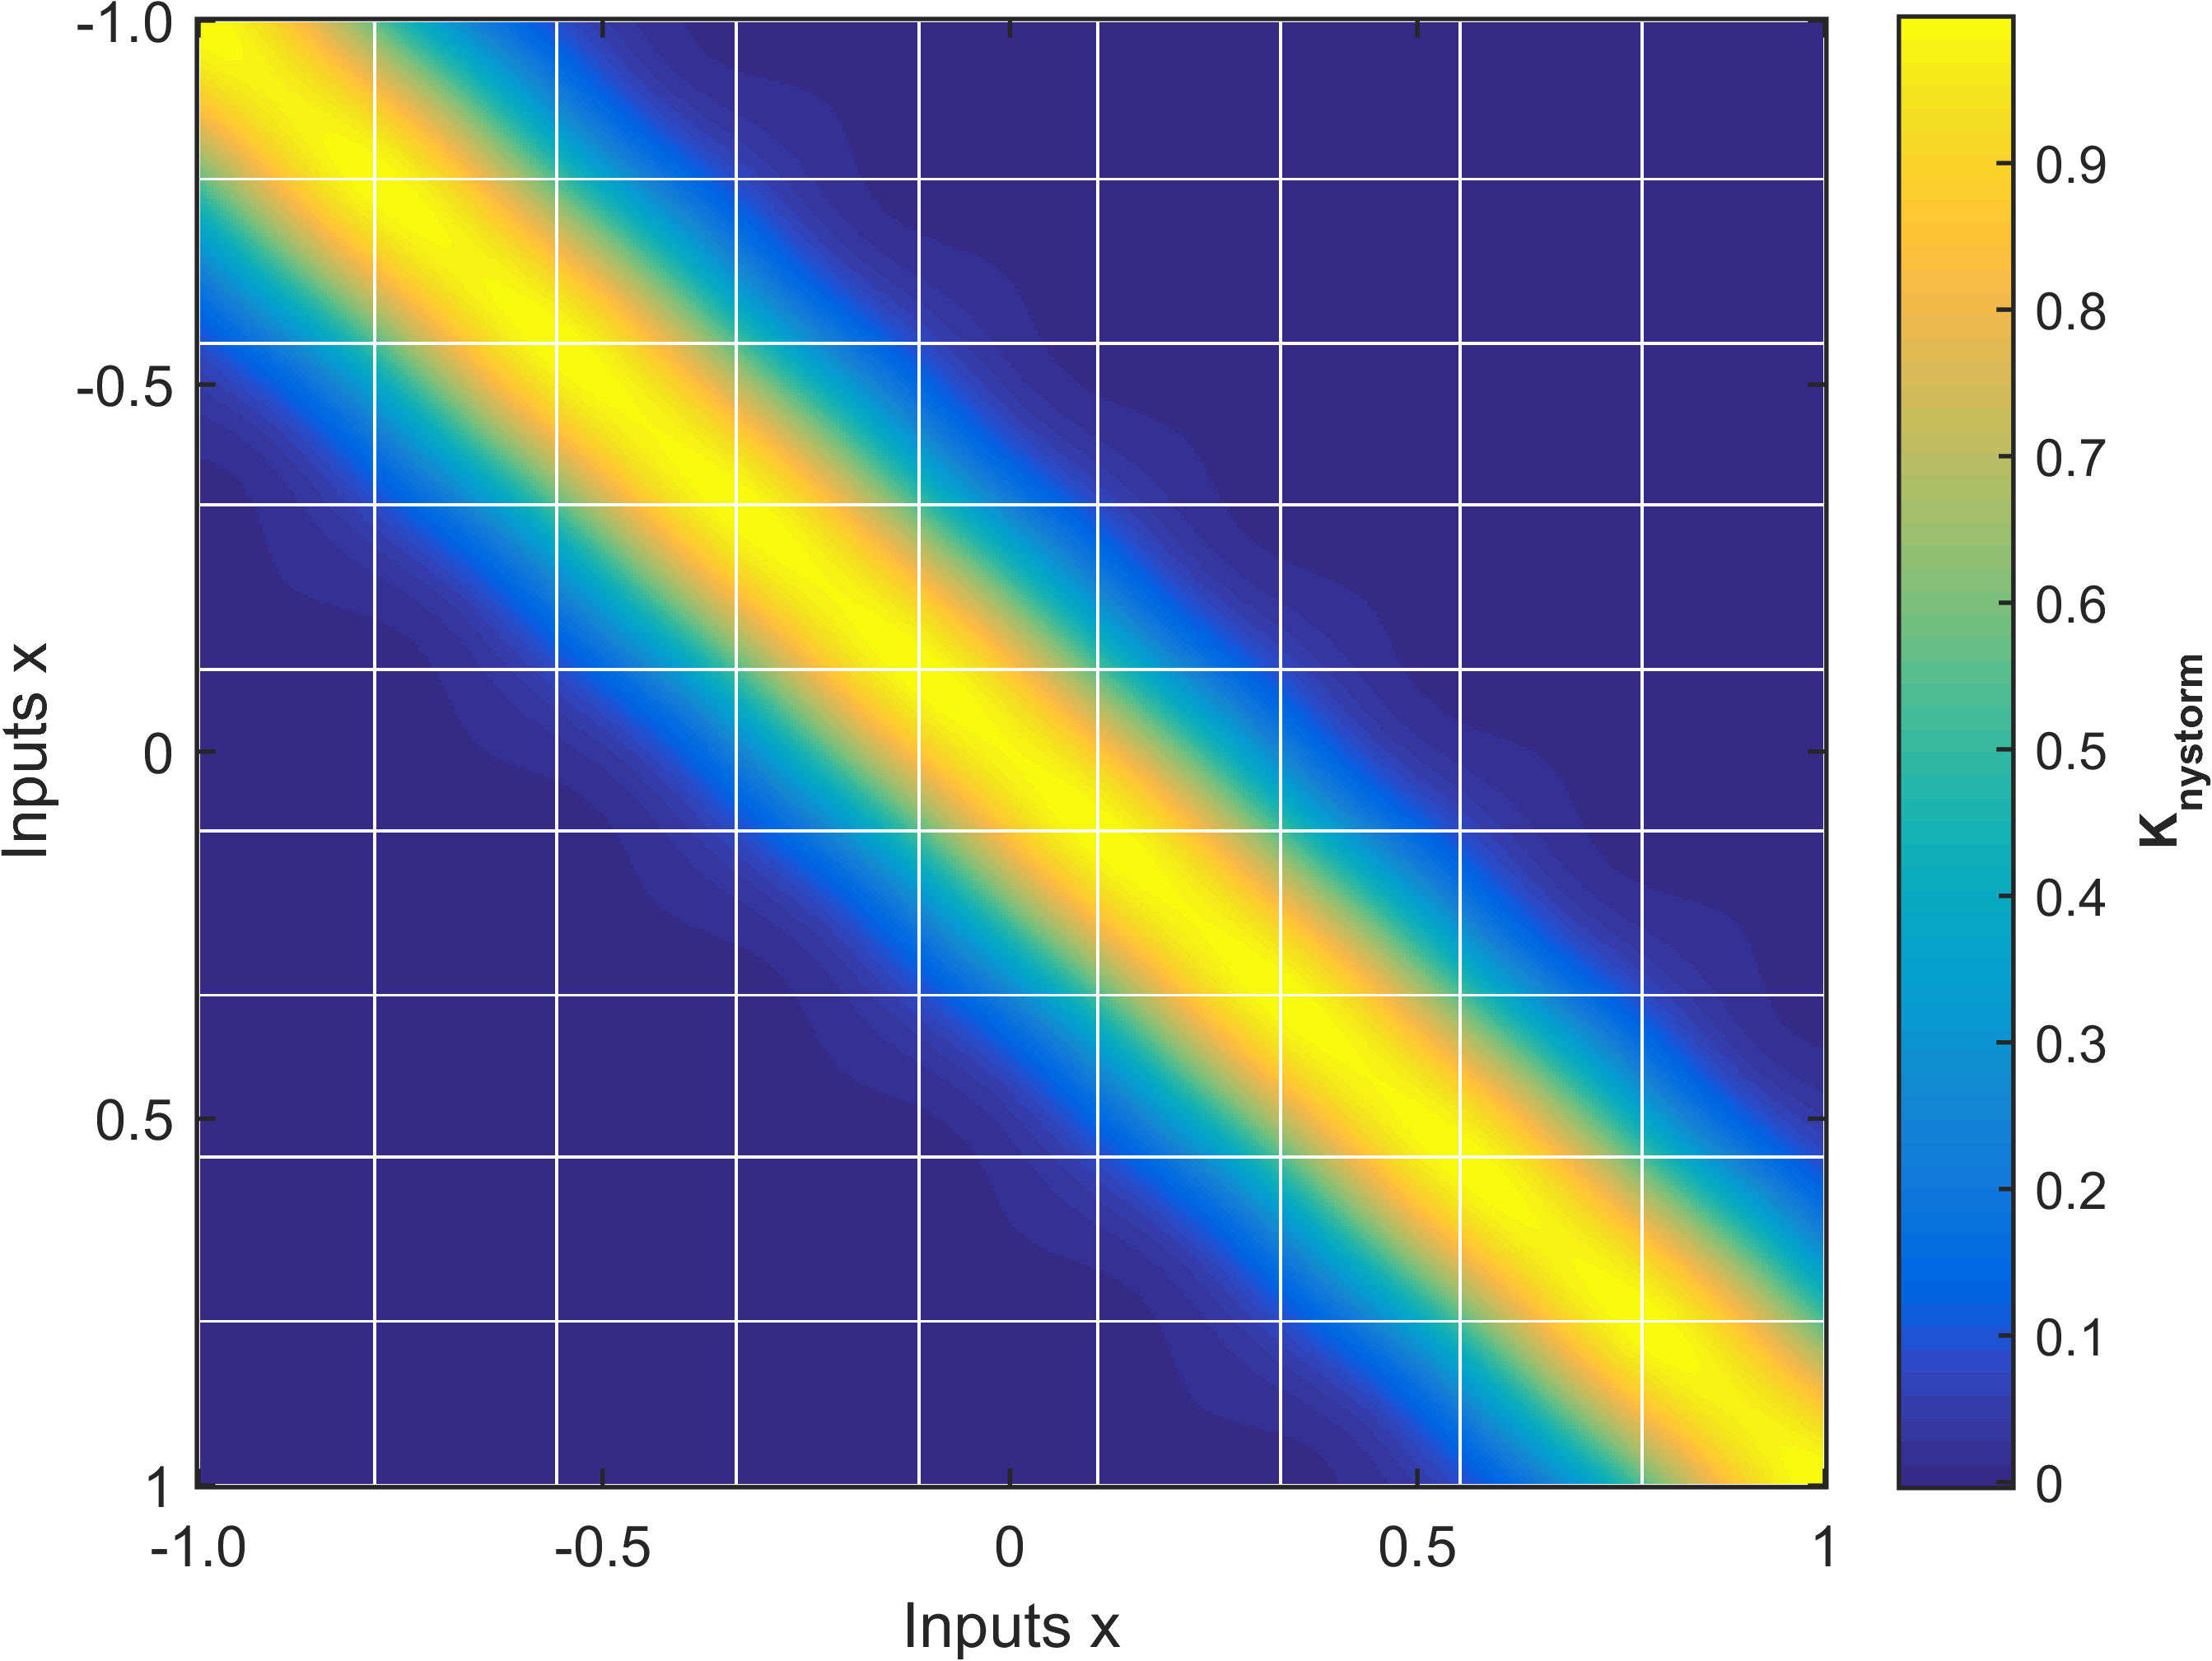
\includegraphics[width=0.45\textwidth]
        {images/nystormSEmatrixUniform}
        \label{subFignystormSEmatrixUniform}
  }\quad
  
       \caption{Approximate Gram matrix for a Standard Exponential kernel using Nystr\"{o}m approximation.}\label{figGPNystormGramMatrix}
\end{figure}

Later, \cite{Snelson06sparsegaussian} proposed the FITC approach which corrects the diagonal terms of the Gram matrix and improves the prediction capabilities (equation \ref{eqnSparseNystormGram}).

\begin{equation}\label{eqnSparseFITCGram}
K_{FITC}(X, X) = diag[K(X, X) - K_{nystorm}(X, X)] + K_{nystorm}(X, X)
\end{equation}

Note, calculating \(diag(K(X, X))\) is an \(\mathcal{O}\left ( N \right )\) operation and thus does not significantly impact the time taken. 


The posterior distribution for the approximate prior can be derived similarly as given in appendix \textbf{add appendix ref} and is a Gaussian. The predictive mean and predictive variance are written as equation \ref{eqNoisyNystormPredictiveMean} and equation \ref{eqNoisyNystormPredictiveCovariance}. Here, \(K_{approximate}(X, X')\) can be the approximated Gram matrix either from the Nystr\"{o}m approximation (equation \ref{eqnSparseNystormGram}) or the FITC approximation (equation \ref{eqnSparseFITCGram}). 
\begin{equation}\label{eqNoisyNystormPredictiveMean}
  \mathbf{E}[f_{approximate}(x_{*})] = K_{Xx_{*}}^{T}( K_{approximate}(X, X') + \sigma^{2}_{n}I)^{-1}Y
  \end{equation}
\begin{equation}\label{eqNoisyNystormPredictiveCovariance}
	Cov[f_{approximate}(x_{*})] = K_{x_{*}x_{*}} - K_{Xx_{*}}^{T}( K_{approximate}(X, X') + \sigma^{2}_{n}I )^{-1} K_{Xx_{*}}
  \end{equation}


By approximating the \(K(X, X)\) using the inducing points we have effectively changed the GP prior. This means that \(X^{m}\) have also become the hyper-parameters of our GP prior. Hence, we should fine-tune locations of \(X^{m}\) and the hyper-parameters \(\theta\) to obtain a good prediction of our data. The marginal likelihood for the approximate prior (equation \ref{equationApproximateML}) be written similarly as equation \ref{equationMarginalLikelihood}.

\begin{equation}\label{equationApproximateML}
    \Pr[Y(X) \mid X, X^{m}, \theta, \sigma_{n}] = \mathcal{N}(0 , K_{approximate}(X, X') + \sigma^{2}_{n}I)
\end{equation}


The maximization of the marginal likelihood in equation \ref{equationApproximateML} with respect to (\(X^{m}\); \(\theta\)), is prone to over-fitting especially when the number of inducing inputs is large. This means that if we keep on increasing the number of inducing points a time will come when we will tend to decrease the accuracy of our predictions on the test data set. The variational approximation (detailed next) approach overcomes this issue of over-fitting by adding a regularization term penalizing over-fitting.

\subsection{Variational Approximation}\label{subSecVariationalApprox} 
The variational approximation does not attempt to approximate the Gram matrix. Instead, it assumes a probability distribution \(q(f)\) of the true posterior distribution \(p(f \mid y)\) and minimizes the distance between the two \cite{Titsias09variationallearning}. 

The \(q(f)\) is written in terms of inducing points (\(X^{m}\)) and the KL divergence \(KL(q||p)\)\footnote{KL divergence is a measure of distance between two probability distributions} is minimized between the variational distribution \(q\) and true distribution \(p\). When we minimize the KL divergence we are making the assumed distribution closer to true distribution and hence improving the values of (\(X^{m}\)) and \(\theta \). This minimization of KL divergence is equivalently expressed as the maximization of the equation \ref{equationLowerBoundVarNLML}

\begin{equation}\label{equationLowerBoundVarNLML}
F_{V} = log(\mathcal{N}[0, \sigma_{n}^{2}I + K_{nystorm}(X, X)]) - \frac{1}{2\sigma_{n}^{2}}Tr(K_{XX} - K_{nystorm}(X, X))
\end{equation}

Notice, the similarity between equation \ref{equationLowerBoundVarNLML} and \ref{eqnSparseNystormGram}. The novelty of the above objective function is that it contains a regularization term: \(- \frac{1}{2\sigma ^{2}}Tr(K_{XX} - K_{nystorm}(X, X))\). Thus, \(F_{V}\) attempts to maximize the marginal likelihood as derived for Nystr\"{o}m approximation and simultaneously minimizes the trace. When the regularization term tends to zero \(K_{XX} - K_{nystorm}(X, X)\), which means that the inducing variables can exactly reproduce the full GP prediction. 

The posterior distribution for variational inference approximation is same as the one derived for Nystr\"{o}m approximation. The difference between Nystr\"{o}m approximation and variational approximation is the improvement in the evaluation parameter while optimizing \(X^{m}\) and \(\theta\). Due to the additional trace term variational inference reduces over-fitting.

\subsection{Experiments}\label{subsecNystromExperiments}
We here conduct experiments on a toy-data set to observe the accuracy of Nystr\"{o}m approximation for varying number and location of inducing points. The basic toolbox used for this paper is GPML provided with \cite{rasmussen2006gaussian} on MATLAB 2014b. All experiments were performed on an Intel quad-core processor with 4Gb RAM. 

10-fold Cross Validation (CV) will be used to assess the performance of the prediction. CV is a technique where the dataset is partitioned as the test set and training set. A model is learned using the training set and Root Mean Square Error (RMSE) is calculated between the prediction and test set as a measure of accuracy. In the 10-fold version of CV, the dataset will be randomly partitioned into 10 subsets containing an equal number of points. Of the 10 subsets, a single subset is retained as the test dataset, and the remaining 9 (10 - 1) subsets are used as training data. The cross-validation process is then repeated 10 times (the folds), with each of the k subsets used exactly once as the validation data.

The toy data set was generated at 1000 input points \(X = \{[-1:0.002:1]\}\) by sampling a random function from a GP\footnote{\((\Pr[Y \mid X, \theta, \sigma_{n}] = GP(0, K_{SE}(X, X', \theta = [1, 0.1]) + (0.3)^{2}I)\)} with zero mean, SE covariance function (\(\theta = [1, 0.1]\)) and noise \(\sigma_{n} = 0.3\). 

Figure \ref{predictionOfm10_242} is the prediction of the GP obtained after Nystr\"{o}m approximation using 10 inducing points. The solid black line defines the mean function, blue region defines 95\% confidence interval (2\(\sigma\)) distance away from the mean. The points denoted by `+' sign are initial locations of inducing points, while the points denoted by `*' sign are locations of inducing points after optimization. The points denoted by `.' are the test points for this fold of the 10-fold CV. 

Notice the inducing points, while initially randomly distributed are later uniformly distributed due to optimization of marginal likelihood. In this case, since the training points are randomly distributed, uniformly distributed inducing inputs are better approximations of the Gram matrix. In cases where training data set tends to be dense in one region and sparse in another region, lesser inducing points get allocated at the dense region and more get allocated at the sparse region. This happens because the information contained in a dense cluster of data-points can be approximated by a fewer data points (points in a neighbourhood are similar (section \ref{subSecCH2Covariance}) \cite{Snelson06sparsegaussian}.

Figure \ref{boxPlotsOfPerformance_242} are 10-fold RMSE box-plots for varying number of inducing points. The box-plots in red are cases when only the hyper-parameters were optimized while inducing inputs were distributed randomly.The box-plots in blue are the cases when both locations of inducing points and hyper-parameters are optimized. The accuracy of prediction improves with increasing number of inducing points. Accuracy is generally better when both locations of inducing points and hyper-parameters are optimized. Note, the noise in the generated toy-data is \(\sigma_{n}=0.3\), hence \(0.3\) is the best achievable RMSE value. Models constructed when optimizing both \(\theta, X^{m}\) reach this RMSE limit for \(M = 20\). After \(M=50\) accuracy is similar for both the optimization routines. As a thumb rule if \(M = \frac{N}{10}\) then randomly distributing the inducing points and optimizing \(\theta\) will be sufficient to give a good prediction \cite{cao2013efficient}. 

\begin{figure}[!ht]
  \centering
    \subfigure[{Posterior between a Nystorm approximated SE prior with 10 inducing inputs and training data. The solid black line defines the mean function, blue region defines 95\% confidence interval (2\(\sigma\)) distance away from the mean. The points denoted by `+' sign are initial locations of inducing points, while the points denoted by `*' sign are locations of inducing points after optimization.}]
  {
        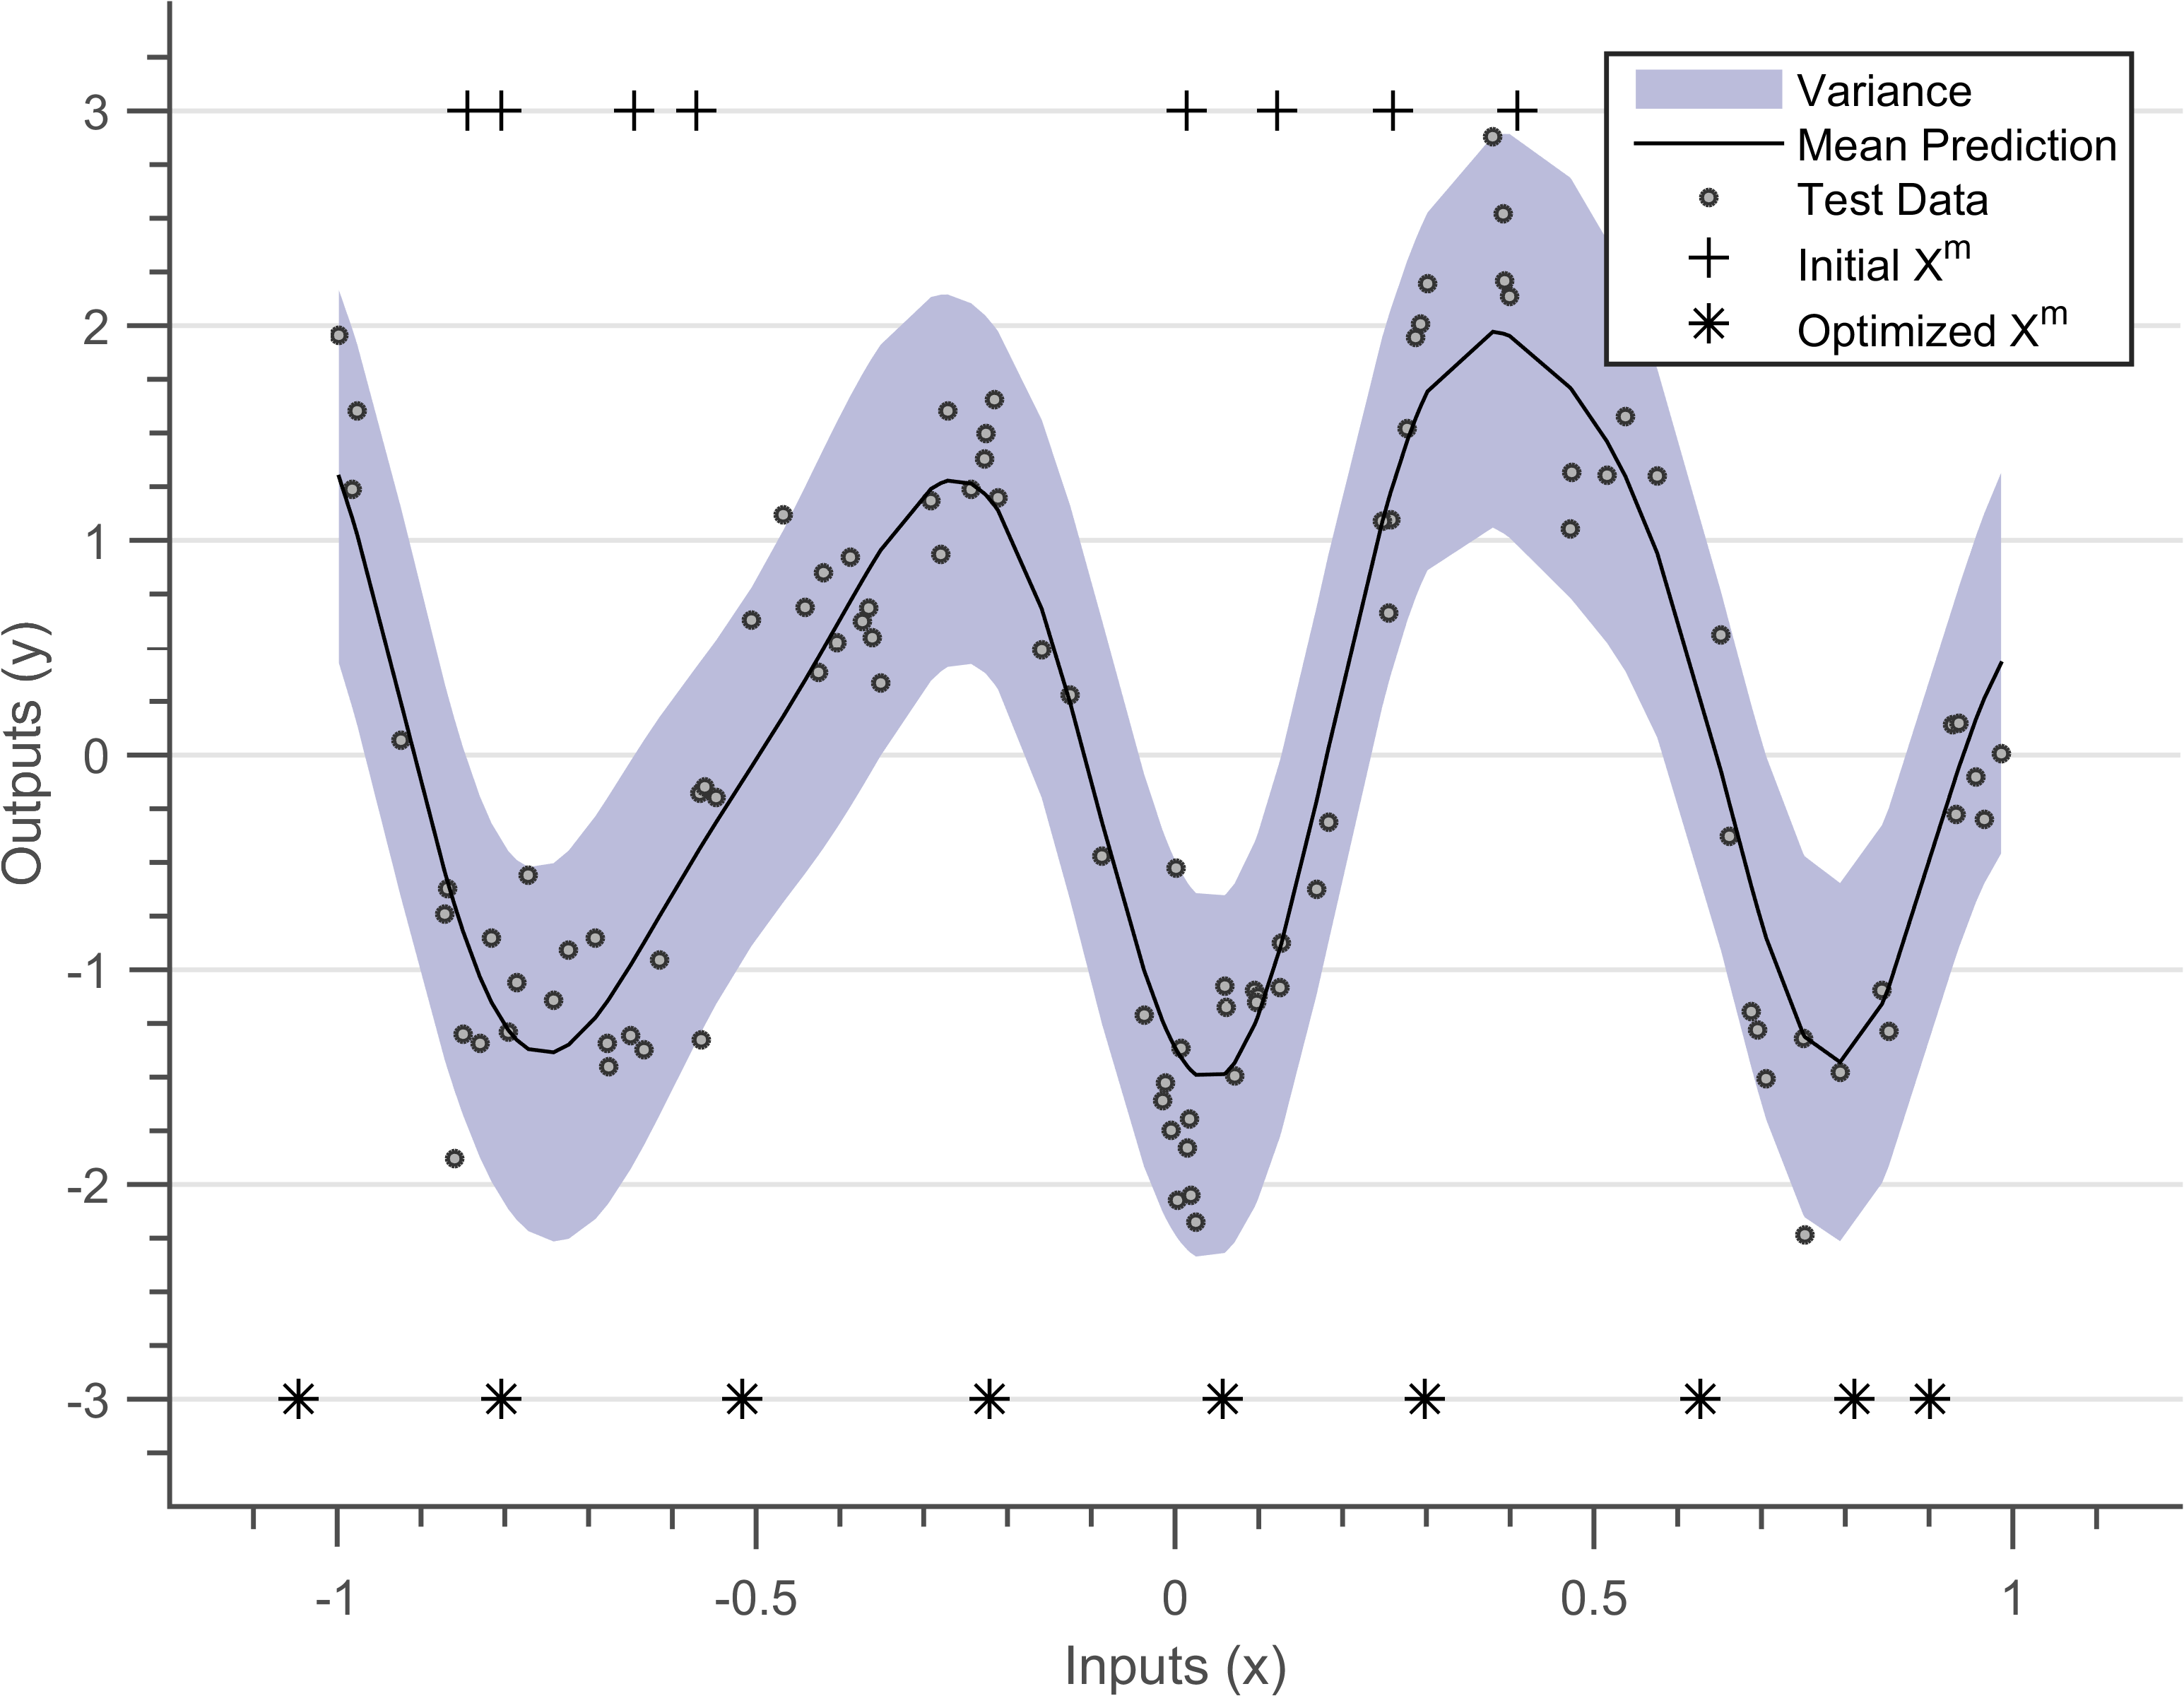
\includegraphics[width=0.45\textwidth]
        {images/predictionOfm10_242}
        \label{predictionOfm10_242}
  }\quad
\subfigure[{10-fold RMSE box-plots for varying number of inducing points. The box-plots in red are cases when only the hyper-parameters \(\theta\) were optimized while inducing inputs were distributed randomly. The box-plots in blue are the cases when both locations of inducing points \(X^{m}\) and hyper-parameters \(\theta\) are optimized. }]
  {
        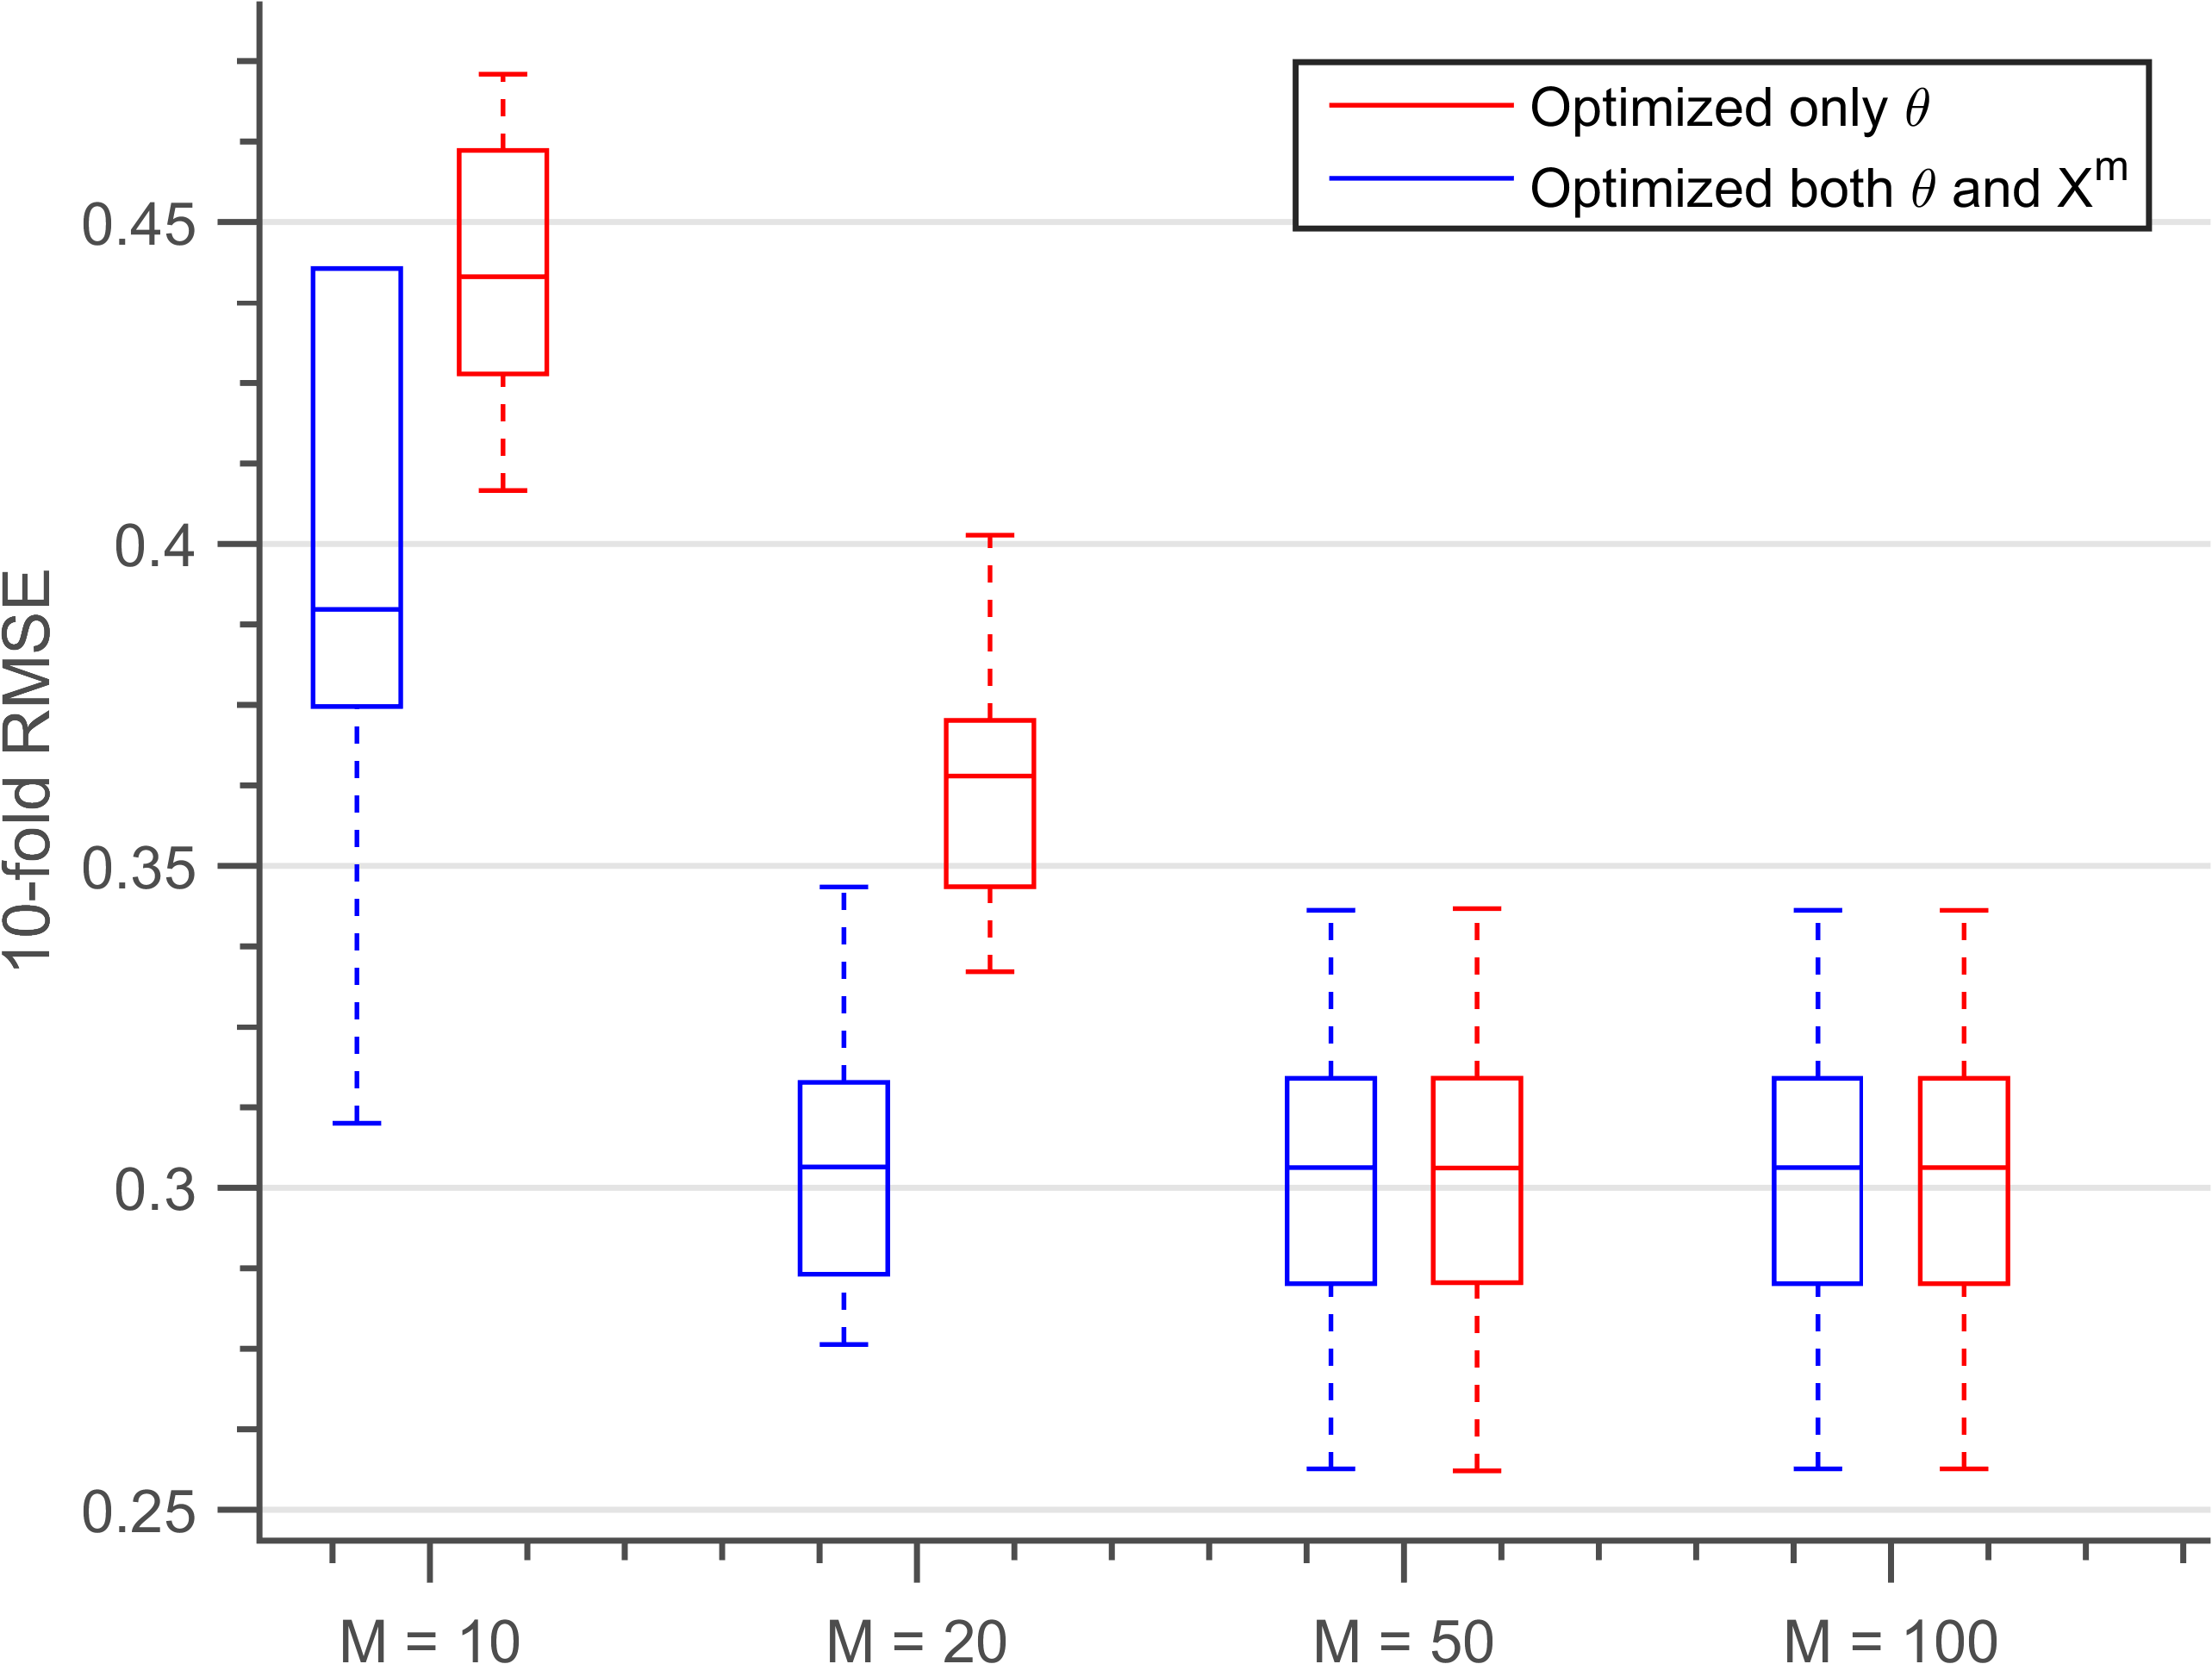
\includegraphics[width=0.45\textwidth]
        {images/boxPlotsOfPerformance_242}
        \label{boxPlotsOfPerformance_242}
  }\quad
  
       \caption{Results of Nystr\"{o}m Approximation on a toy-data set of size \(N=1000\) }\label{figGPPredictionNystorm}
\end{figure}

Global low-rank approximations are best suited for the case of spread out Gram matrices (example high length-scale SE priors). We have seen three types of low-rank approximation algorithms in this section. While Nystr\"{o}m and FITC approximations are the simplest method to approximate Gram matrix, finding optimal locations of the inducing points can often lead to over-fitting. We then, look at variational approximation procedure which adds a regularization term while finding inducing points thereby penalizing over-fitting. The lower computational cost due to sparse approximations, scales sparse GPs to the training set of sizes \(N \sim \mathcal{O}(5 \times 10^5)\). \cite{Gal2014Distributed} propose a distributed architecture for scaling variational sparse GPs. In the next section we look at how to approximate Gram matrices using mixture of experts, this enables us to massively scale GPs to sizes \(N > \mathcal{O}(10^6)\) by exploiting distributed architecture.

\section{Distributed Gaussian Process}\label{secDgp}
In the year 2006 Netflix prize was launched, teams from all over the world competed in the competition to make the best video recommendation algorithm. As the competition progressed teams figured out that performance increases upon combining algorithms developed by multiple teams. The winner and the runner-up were stacked learners of over 100 algorithms. Creating model ensembles (also called mixture of experts) is now a standard practice in many learning competitions \cite{bauer1998empirical}. 

Mixture of experts methods in GPs use bagging, where subsets of data are generated, individual GPs are trained on these subsets and their results are finally combined \cite{chen2009bagging}. If the data set is partitioned  into \(N_{experts}\) subsets such as $\mathcal{D}^{(i)} = {X^{(i)}, Y^{(i)}}, i \in 1, \ldots N_{experts}$. Each subset of data learns an individual GP model, which can be combined together to give final predictions . Due to individual learning choosing hyper-parameters and calculating prediction become easily parallel-able and indifferent to the computational infrastructure. 

Initially, this mixture of local models was used to highlight local features in the data \cite{rasmussen2002infinite}. \cite{ng2014hierarchical} propose to use the mixture of experts methodology to speed up prediction in a Gaussian Process. Instead of learning a different GP for each subset, we tie all the different experts using one single set of hyperparameters. This is equivalent to assuming one single GP for the whole data-set such that there is no correlation across experts, i.e. the experts are independent of each other. This tying of experts greatly reduces the number of hyper-parameters to optimize, acts as a regularization and inhibits over-fitting. Equation \ref{distributedGPPrior} denotes an independent GP prior for each expert \(\mathcal{D}^{(i)}\) such that the hyper-parameters \(\theta\) and \(\sigma_{n}\) are same for all experts.

\begin{equation}\label{distributedGPPrior}
    \Pr[y^{(i)} \mid x^{(i)}, \theta, \sigma_{n}] = GP(0, K(x^{(i)}, x^{(i)'}, \theta) + \sigma^{2}_{n}I) 
\end{equation}

Figure \ref{subFigdistributedKernelRandomExperts} is an approximate Gram matrix using distributed GP approximation for a Standard Exponential (SE) Kernel with \((\theta = [1, 0.2])\) (figure \ref{subFigcovSEmatrix_1}) at the input points \(X^{*} = \{[0:0.02:1]\}\). 5 experts each having 100 points are chosen, points in the experts are distributed randomly, this gives the approximate Gram matrix scattered shape. Figure \ref{subFigDistributedKernel} is an approximate Gram matrix using distributed GP approximation of the matrix in figure \ref{subFigcovSEmatrix_1} and uniformly distributed experts. 5 experts each having 100 points are chosen, The first expert has first set of 100 points, the second expert has the second set of 100 points and so on. The Gram matrix with randomly chosen experts has a more global nature but lacks many high variance regions. The Gram matrix for uniformly chosen experts retains more local features. Inversion of this Gram matrix is an operation of complexity \(\mathcal{O}(N_{experts}P^{3})\), where \(P\) is the number of points in an expert.

\begin{figure}[!ht]
  \centering
    \subfigure[{Approximated Gram matrix using distributed GP approximation for a Standard Exponential (SE) Kernel with \((\theta = [1, 0.2])\) (figure \ref{subFigcovSEmatrix_1}) at the input points \(X^{*} = \{[0:0.02:1]\}\). Points in the experts are distributed randomly, this gives the approximate Gram matrix scattered shape.}]
  {
        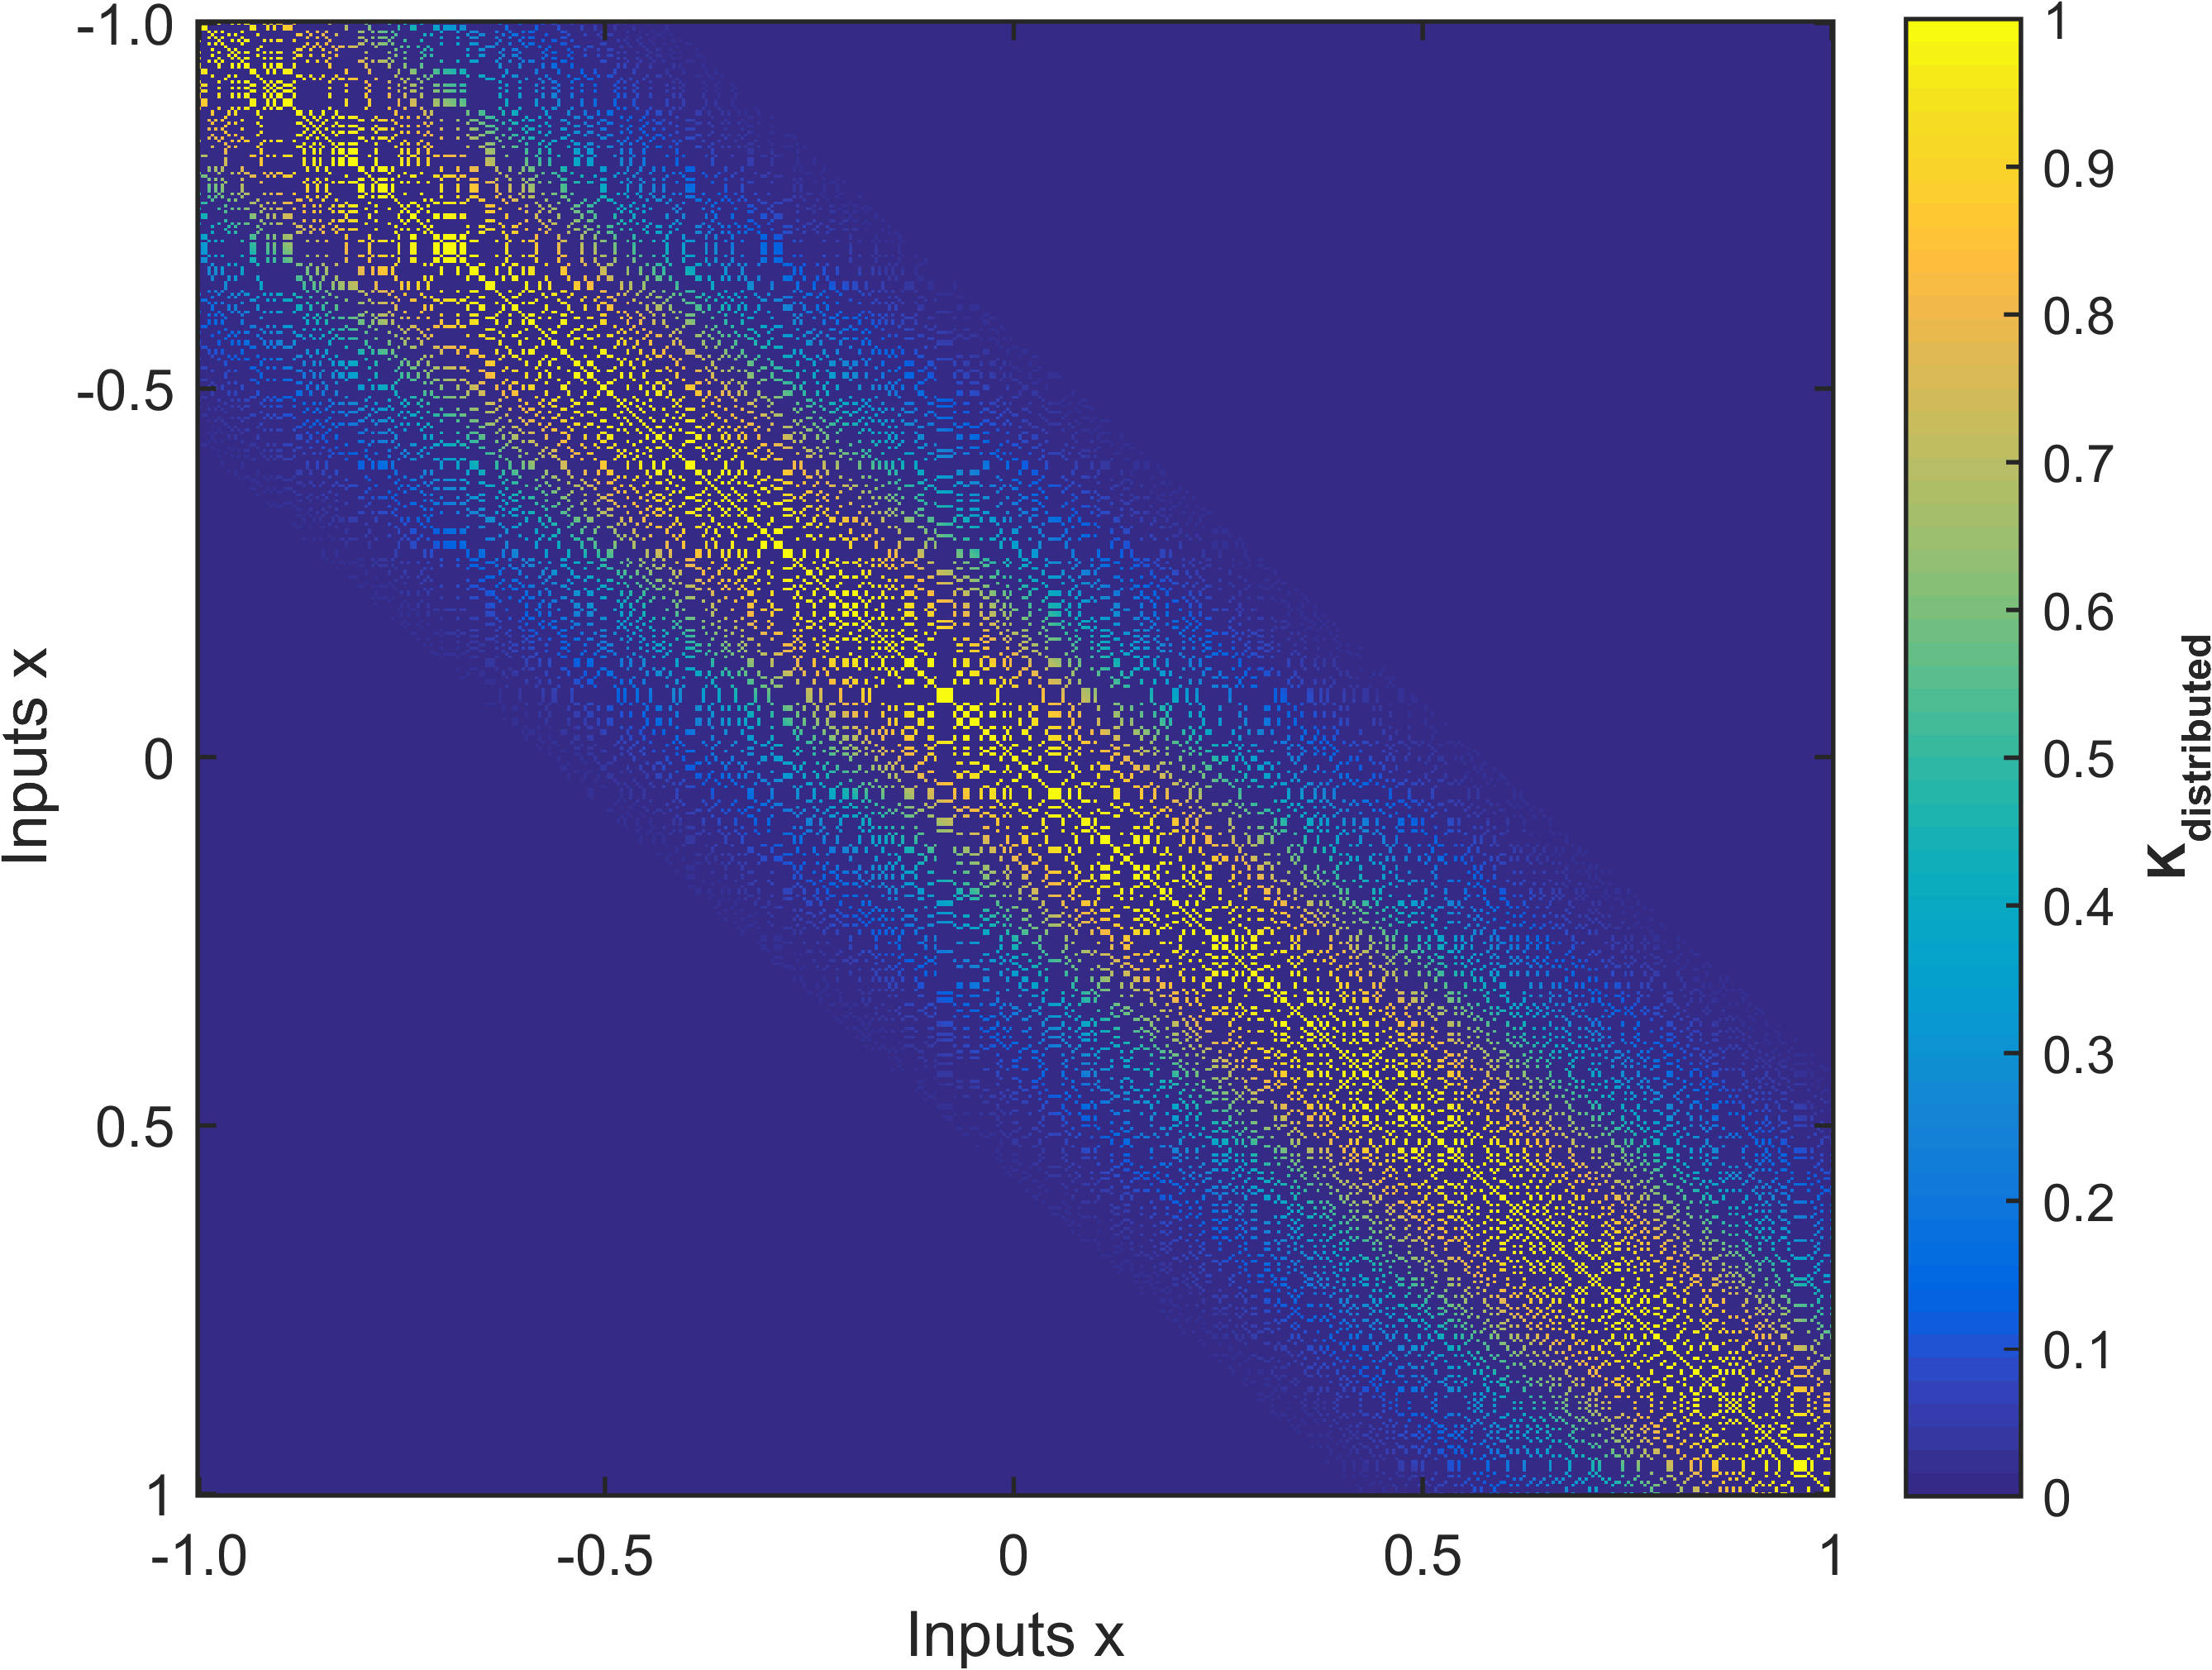
\includegraphics[width=0.45\textwidth]
        {images/distributedKernelRandomExperts}
        \label{subFigdistributedKernelRandomExperts}
  }\quad
\subfigure[{Approximated Gram matrix using distributed GP approximation for a Standard Exponential (SE) Kernel with \((\theta = [1, 0.2])\) (figure \ref{subFigcovSEmatrix_1}) at the input points \(X^{*} = \{[0:0.02:1]\}\). Points in the experts are distributed uniformly. We can observe that covariance across experts goes to zero.}]
  {
        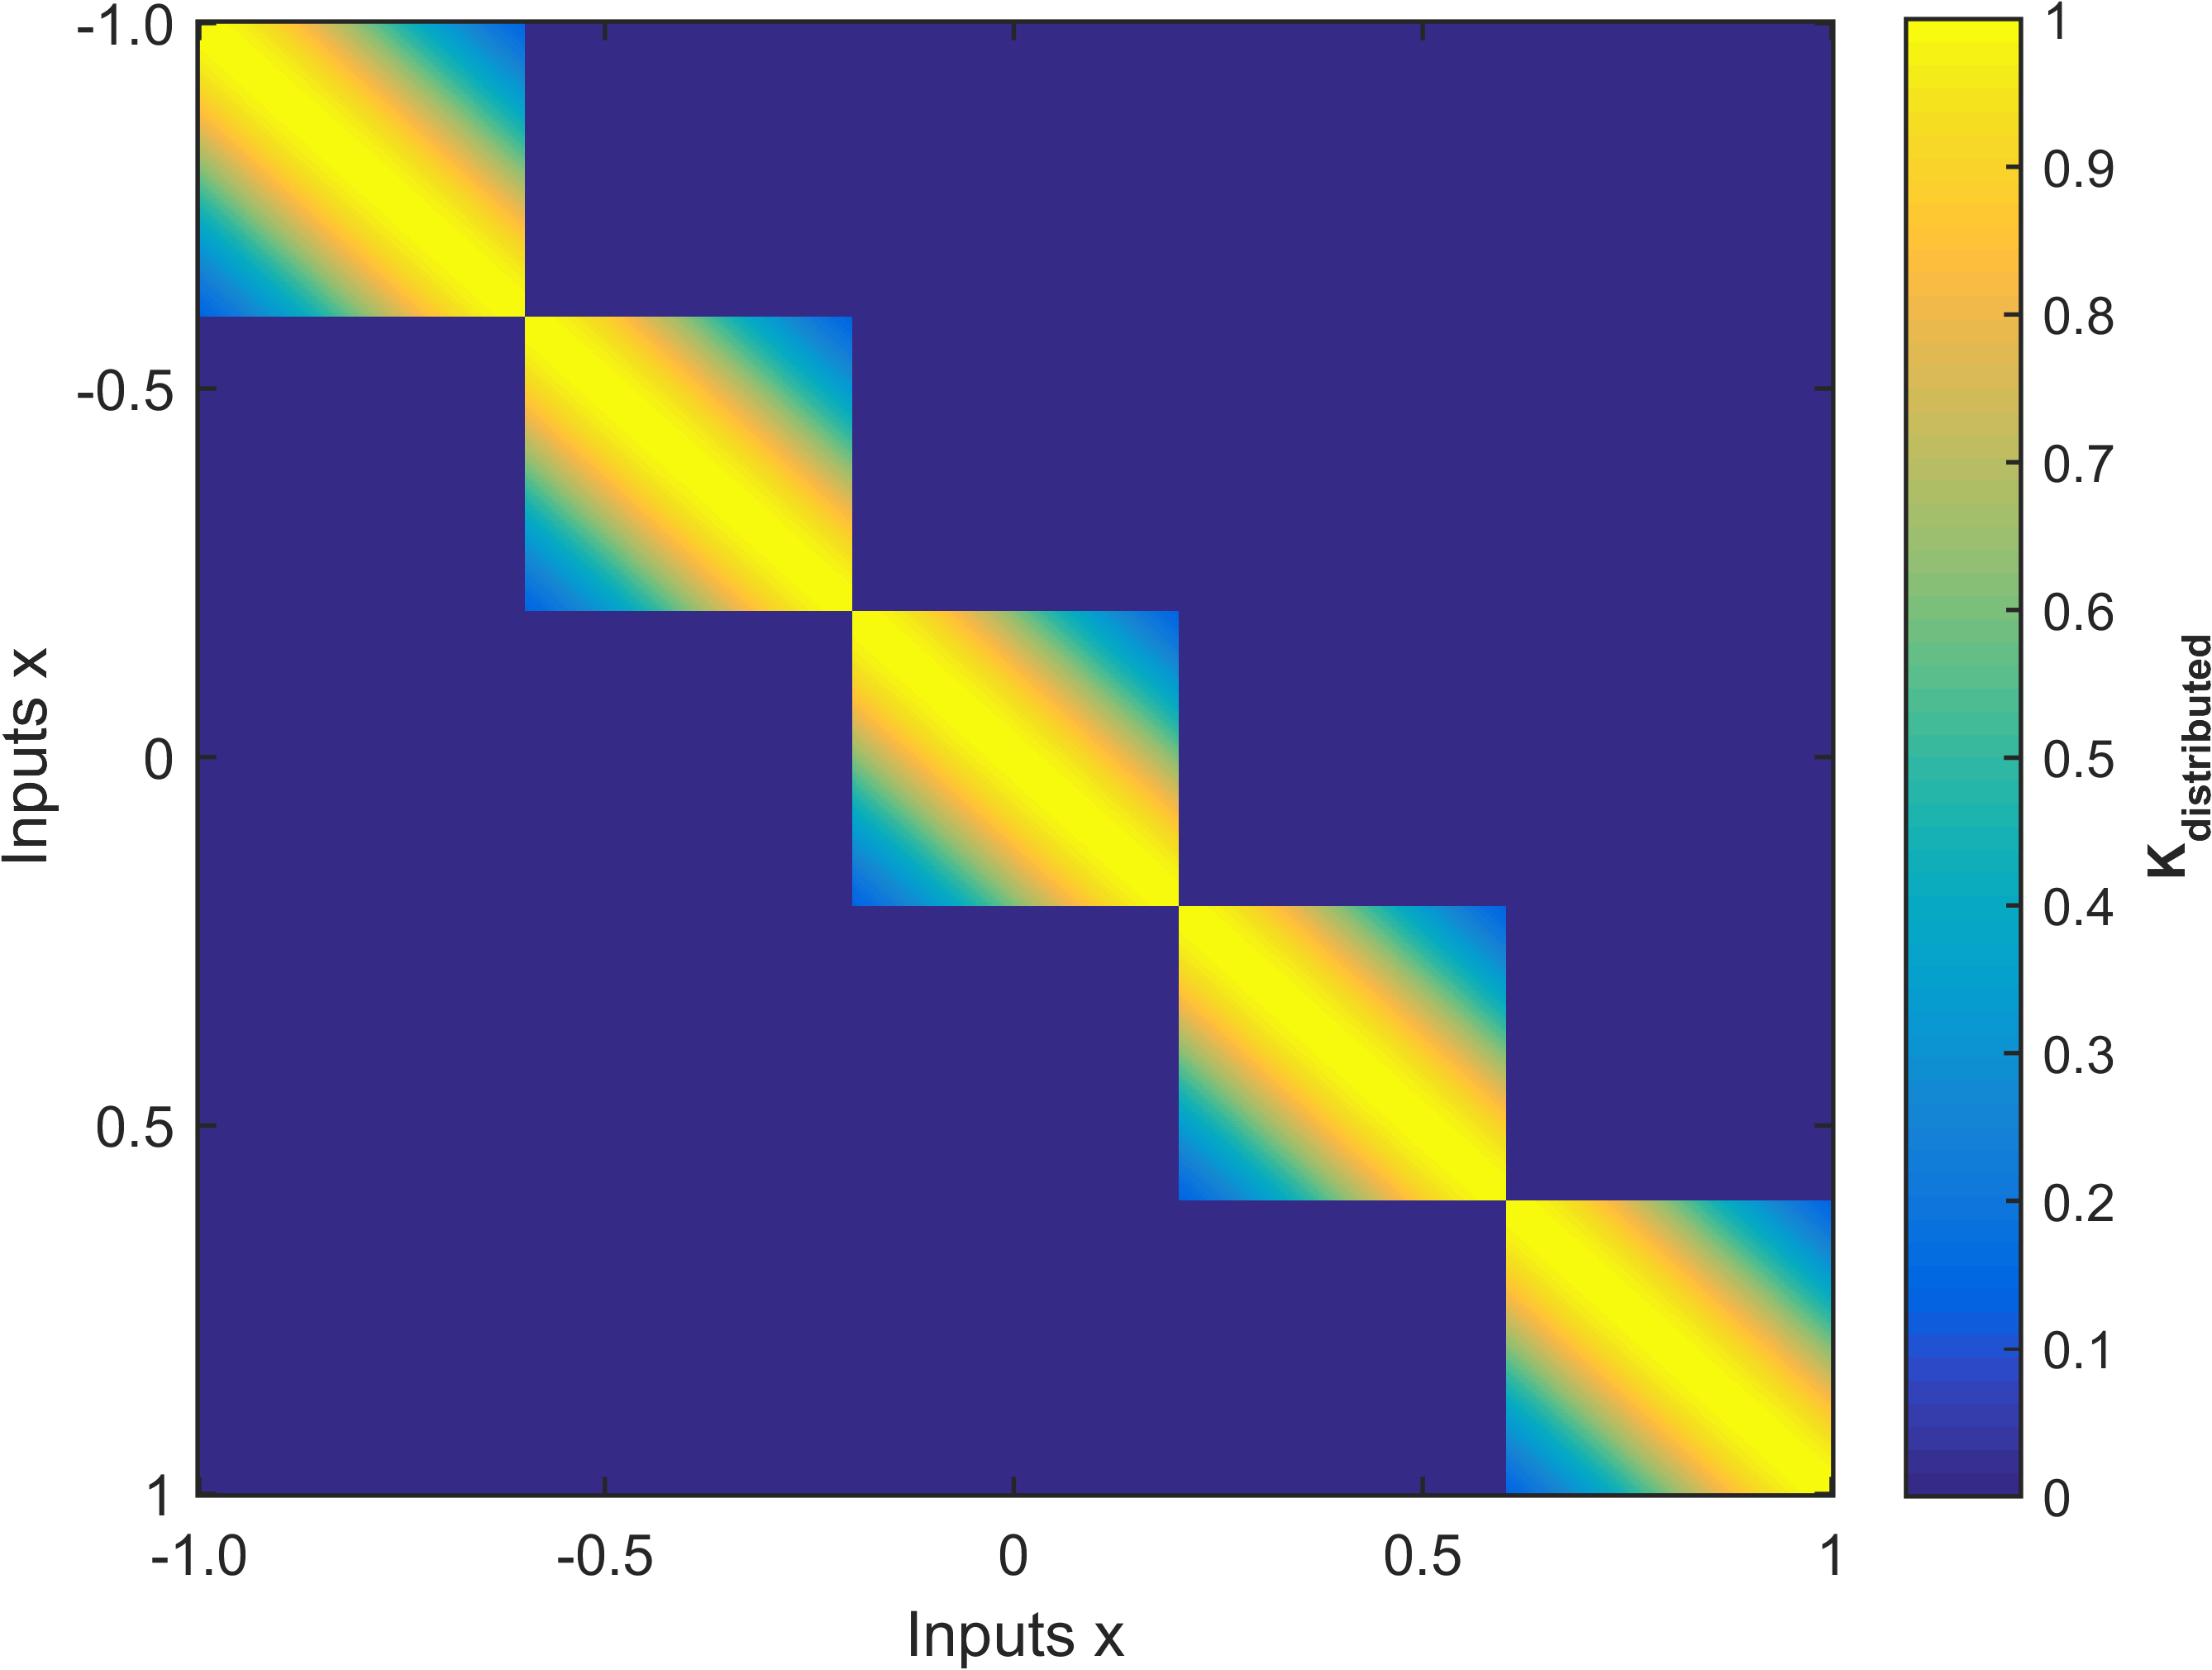
\includegraphics[width=0.45\textwidth]
        {images/distributedKernel}
        \label{subFigDistributedKernel}
  }\quad
  
       \caption{Approximate Gram matrix for a Standard Exponential kernel using mixture of experts.}\label{figGPApproximateDGPMatrix}
\end{figure}

Since the experts are independent of each other, we can construct a posterior distribution for each expert (equations \ref{eqPredictiveMeanIndividualExpert} and \ref{eqPredictiveCovarianceIndividualExpert}). In the following equations \(m^{(i)}(x_{*})\) and \(\sigma^{(i)}(x_{*})\) are the mean and covariance predictions from expert \(i\) at point \(x_{*}\).  

\begin{equation}\label{eqPredictiveMeanIndividualExpert}
  m^{(i)}(y(x_{*})) = K_{x^{(i)}x_{*}}^{T}( K_{x^{(i)}, x^{(i)'}} + \sigma^{2}_{n}I)^{-1}y^{(i)}
  \end{equation}
\begin{equation}\label{eqPredictiveCovarianceIndividualExpert}
	\sigma^{(i)}(y(x_{*})) = K_{x_{*}x_{*}} - K_{x^{(i)}x_{*}}^{T}( K_{x^{(i)}, x^{(i)'}} + \sigma^{2}_{n}I )^{-1} K_{x^{(i)}x_{*}}
  \end{equation}

\subsection{Combining experts}\label{subSecCombiningExperts}
There exist several methods in the literature on how to combine these individual posterior predictions of the experts to give the final posterior distribution. The Product of Experts model uses the independence assumption between experts and multiplies the individual posterior distribution\footnote{\(\Pr[y(x_{*}) \mid x_{*}, \mathcal{D}, \theta] \propto \prod \Pr[y^{(i)} \mid x^{(i)}, \mathcal{D}^{(i)}, \theta]\)}, but these predictions tend to be overconfident. Another method called the generalized Product of Experts (gPOE) assigns a participation factor to each expert based on the amount of uncertainty in prediction (more confident experts have higher say in prediction)\cite{cao2014generalized}. The Bayesian Committee Machine (BCM) imposes the independence assumption between each expert pair using Bayes Rule, but can result in bad predictions when leaving data regime \cite{tresp2000bayesian}. 

This thesis will use robust Bayesian Committee Machine (rBCM) model to combine the posterior distributions of experts \cite{deisenroth2015distributed}. The rBCM model is an amalgamation of all the above three mentioned methods, it combines the confidence weighting parameter of gPOE with the Bayesian formulation in BCM technique to generate the following posterior distributions.

\begin{equation}\label{eqCovarianceDGP}
    Cov(y(x_{*}))^{^-2} = \sum_{i} \beta_{i}\sigma_{(i)}^{-2} + (1- \sum_{i} \beta_{i})(K_{x_{*}x_{*}})^{-2}
\end{equation}
\begin{equation}\label{eqMeanDGP}
    m(y(x_{*})) = (Cov(y(x_{*})))^{-2}\sum_{i} \beta_{i}(\sigma^{(i)})^{-2}m^{(i)}(x_{*})
\end{equation}

\(K_{x_{*}x_{*}}\) is the auto-covariance of the prior at prediction point \(x_{*}\). \(\beta_{k}\) determines the influence of experts on the final predictions \cite{cao2014generalized} and is given as \(\beta_{i} = \frac{1}{2}(\log K_{x_{*}x_{*}}^{2} - \log(\sigma^{(i)})^{2})\). Experts which are very confident of their predictions at \(x_{*}\) will tend to have low \(\sigma^{(i)}\) thereby leading to a higher influence factor \(\beta_{i}\).

Due to the independence assumption, the marginal likelihood can be written as a sum of individual likelihoods and then can be optimized to find the best-fit hyperparameters. By approximating the \(K(X, X)\) in terms of \(\mathcal{D}^{(i)}\) and \(N_{experts}\) we have again changed the GP prior. This means that the number of experts \(N_{experts}\) and clustering of points in individual experts also impact the prediction capabilities of GP. The below equation \ref{eqDGPNLML} describes the formulation for marginal likelihood. 

\begin{align}\label{eqDGPNLML}
    \log \Pr[y \mid X, \mathcal{D}, \theta] \approx \sum_{k=1}^{N_{experts}} \log \Pr[y^{(i)}\mid X^{(i)}, \theta]
 \end{align}

Maximizing the above log-marginal likelihood will give the optimal values of hyper-parameters. Points in the experts can be distributed either randomly or using a clustering scheme (eg. k-means clustering\footnote{k-means algorithm clusters close by points in one cluster. The notion of closeness is defined by some measure of distance}) for stationary kernels\footnote{stationary kernels are only a function of d = |x-x'|} k-means clustering should be preferred. The k-means algorithm clusters points based on a measure of distance, points in separate clusters are far away from each other when compared to points in the same cluster. This means that the covariance (for stationary kernels) between separate clusters is significantly lower when compared to points in same cluster. Hence, the cross-covariance across separate clusters can be more easily assumed to be zero.

\subsection{Experiments}\label{subSecDistributedExperiments}
We again conduct experiments on a toy-data set, this time to observe the accuracy of distributed GP approximation for varying number of experts. 

Again the 10-fold Cross Validation (CV) will be used to assess the performance of the prediction. The same toy-data set as used in section \ref{subsecNystromExperiments} was used to perform the experiments in this section (1000 data-points from \(\Pr[y \mid X, \theta, \sigma_{n}] = GP(0, K_{SE}(X, X', \theta = [1, 0.1]) + (0.3)^{2}I)\).

Figure \ref{predictionOfm10_243} is the prediction of the GP obtained after distributed approximation using 9 experts and k-means clustering. The solid black line defines the mean function, blue region defines 95\% confidence interval (2\(\sigma\)) distance away from the mean. The colored points in the points denoted by `*' at the bottom show how different points are distributed across experts, similar colored points belong to one expert. The data denoted by `.' is the test data for one fold of the 10-fold CV. 

The points across experts are uniformly distributed, as can be observed by the coloring scheme. Since the training points are almost uniformly distributed, the k-means algorithm will cluster the points uniformly. Actually, the training and test set used in figures \ref{predictionOfm10_243} and \ref{predictionOfm10_242} are same. Notice how Nystr\"{o}m approximation has a global smooth shape while the distributed GP approximation retains the local features of the data set. 

Figure \ref{boxPlotsOfPerformance_243} are 10-fold RMSE box-plots for different number of \(P\). The box-plots in red are cases when the points are distributed using k-means clustering. The box-plots in blue are the cases when points are distributed randomly. The accuracy of prediction improves with increasing number of points in an expert. Note, the noise in the generated toy-data is \(\sigma_{n}=0.3\), hence \(0.3\) is the best achievable RMSE value. Accuracy is slightly better when experts are distributed using k-means clustering, both being very close to the \(0.3\) RMSE limit. As a thumb-rule setting \(P = N/10\) and optimizing the hyper-parameters (\(\theta\)) is a good enough approximation. 


\begin{figure}[!ht]
  \centering
    \subfigure[{Prediction of the GP obtained after distributed approximation using 9 experts and k-means clustering. The solid black line defines the mean function, blue region defines 95\% confidence interval (2\(\sigma\)) distance away from the mean. The colored points in the points denoted by `*' at the bottom show how different points are distributed across experts, similar colored points belong to one expert. The data denoted by `.' is the test data for one fold of the 10-fold CV. }]
  {
        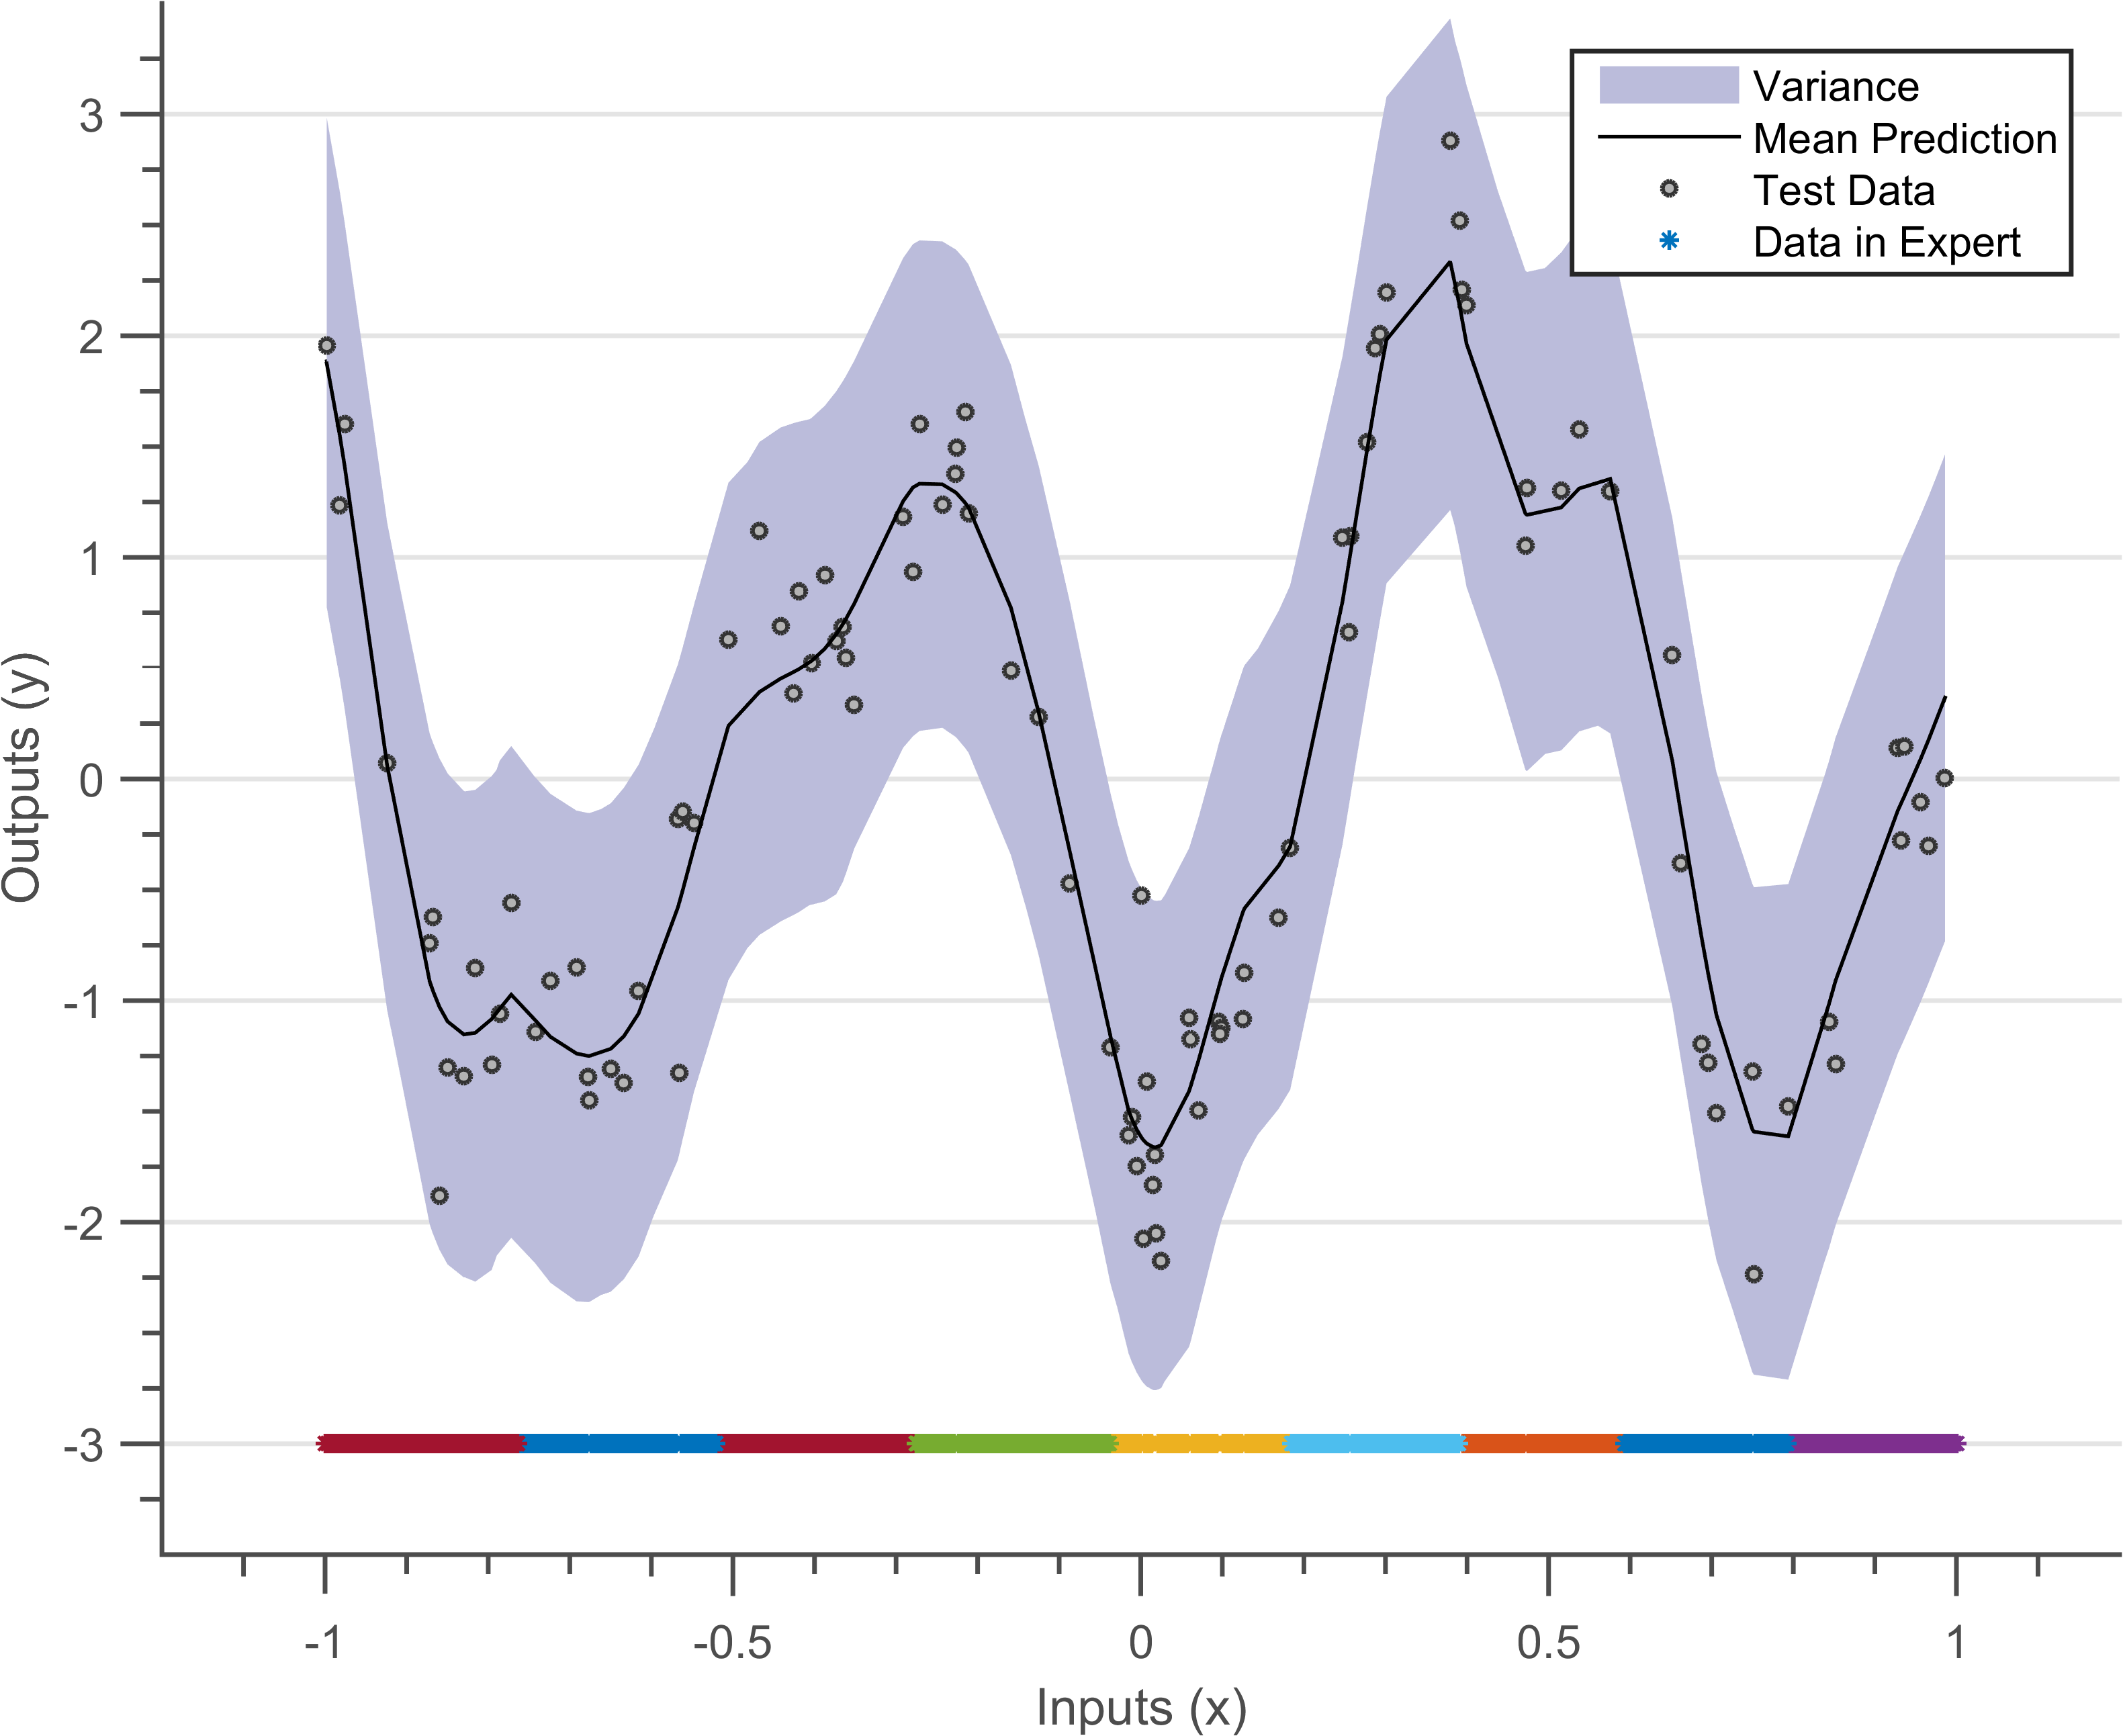
\includegraphics[width=0.45\textwidth]
        {images/predictionOfm10_243}
        \label{predictionOfm10_243}
  }\quad
\subfigure[{10-fold RMSE box-plots for different number of points across. The box-plots in red are cases when only the hyper-parameters when the points are distributed using k-means clustering. The box-plots in blue are the cases when points are distributed randomly. The accuracy of prediction improves with increasing number of points in an expert}]
  {
        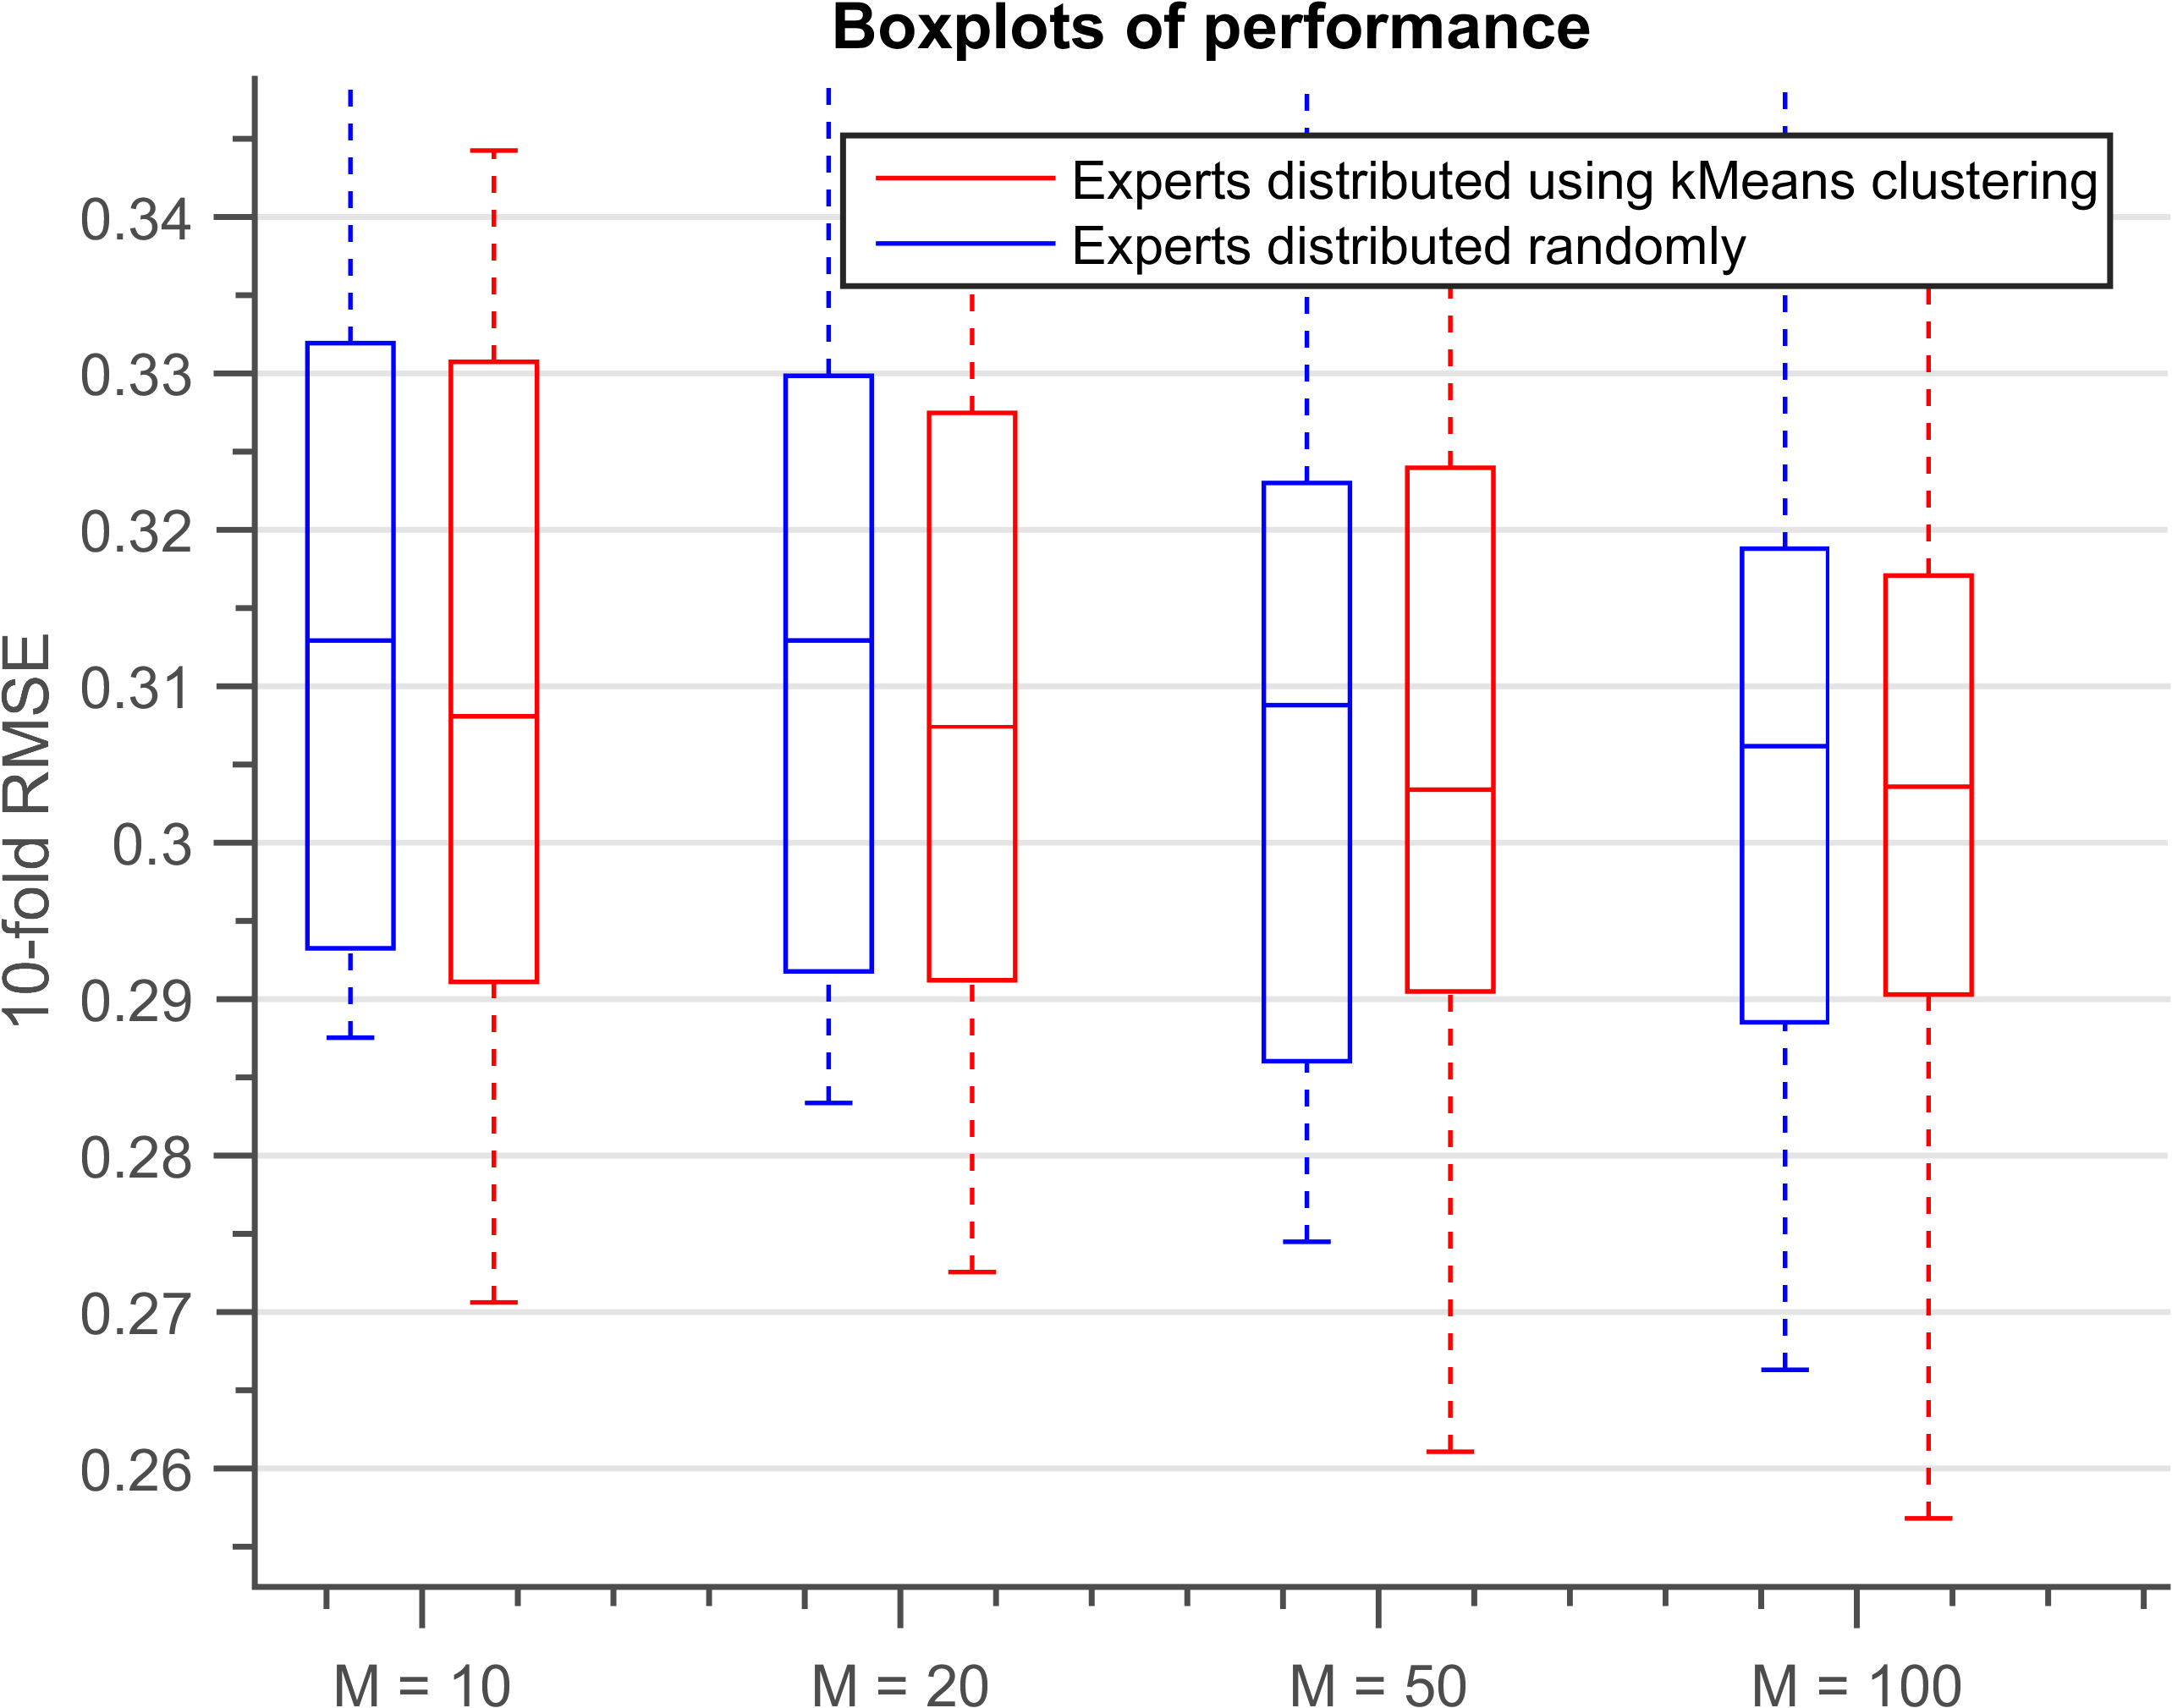
\includegraphics[width=0.45\textwidth]
        {images/boxPlotsOfPerformance_243}
        \label{boxPlotsOfPerformance_243}
  }\quad
  
       \caption{Results of distributed GP Approximation on a toy-data set of size \(N= 1000\)}\label{figGPPredictionDistributed}
\end{figure}

\section{Discussion}
The calculation of posterior distribution in GPs becomes computationally intractable for large data sets. Calculating the precision matrix is an operation of computational complexity \(\mathcal{O}(N^{3})\), putting a limit of \(N \sim 10^4\) data points for model building. This chapter \ref{chapSparseGPRegression} describes the state of art for scaling up GPs for regression tasks. There exist two methods to scale up GPs, the first called sparse methods which uses a set of inducing inputs to reduce the computational cost of calculating the precision matrix. The second called distributed GP which divides the data set into another set of smaller datasets called experts, distributing the model building into several batches. 

Sparse methods use Nystr\"{o}m approximation rewriting the Gram matrix as equation \ref{subSecSamplingFunctionsGPPrior}, thereby reducing the computational complexity to \(\mathcal{O}(NM^{2})\) (M << N), \(M\) being the number of inducing points. Through experiments on a toy-dataset it can be shown that we can set \(M \sim N/10\) for randomly distributed inducing points and \(M \sim N/50\) when we optimize the locations of inducing points. This approximation pushes the limit of GP Regression to \(N \sim 10^6\) data points. Distributed GPs distributes the GP Regression tasks into several batches, thereby reducing the computational complexity to \(\mathcal{O}(NP^{3})\) (P<<N), \(P\) being the number of points in an expert. Through experiments on a toy-dataset we demonstrate that \(P \sim N/100\) does not effects the regression task significantly. In fact we can further reduce \(P\) if we enable repetition of points between experts. This enables to scale GPs to any number of data-points, we will demonstrate this by running a GP regression on millions of data-points in this manuscript (section \ref{}). 

There are several reasons why GPs should be preferred to perform regression tasks. GPs provide a probabilistic framework to define a family of functions, while the covariance functions allows to incorporate a wide range of assumptions (Chapter \ref{chapStructureWithCovariance}). GPs are computationally tractable, given a covariance function and observations, the predictive distribution can be calculated exactly. By providing a closed form expression of marginal likelihood GPs provide a powerful method to automatically select hyperparameters. Although GPs suffer in presence of large data sets, there exist several approximate methods to scale GPs to millions of data points. 






\part{Incorporating structure in Gaussian Process Regression}
\include{04-structureThroughCovariance}

\part{Incorporating multiple outputs Gaussian Process Regression}
\include{05-addingEquations}
\include{06-multiTaskExtrapolation}

\appendix

\bibliographystyle{authoryear-fr}
\bibliography{references}

\clearpage

%%%%%%%%%%%%%%%%
%%% Abstract %%%
%%%%%%%%%%%%%%%%

\thispagestyle{empty}

\vspace*{\fill}
\noindent\rule[2pt]{\textwidth}{0.5pt}\\
{\textbf{Résumé ---}}
Lorem ipsum dolor sit amet, consectetur adipiscing elit. Sed non risus. Suspendisse lectus tortor, dignissim sit amet, adipiscing nec, ultricies sed, dolor. Cras elementum ultrices diam. Maecenas ligula massa, varius a, semper congue, euismod non, mi. Proin porttitor, orci nec nonummy molestie, enim est eleifend mi, non fermentum diam nisl sit amet erat. Duis semper. Duis arcu massa, scelerisque vitae, consequat in, pretium a, enim. Pellentesque congue. Ut in risus volutpat libero pharetra tempor. Cras vestibulum bibendum augue. Praesent egestas leo in pede. Praesent blandit odio eu enim. Pellentesque sed dui ut augue blandit sodales. Vestibulum ante ipsum primis in faucibus orci luctus et ultrices posuere cubilia Curae; Aliquam nibh. Mauris ac mauris sed pede pellentesque fermentum. Maecenas adipiscing ante non diam sodales hendrerit. Ut velit mauris, egestas sed, gravida nec, ornare ut, mi. Aenean ut orci vel massa suscipit pulvinar. Nulla sollicitudin. Fusce varius, ligula non tempus aliquam, nunc turpis ullamcorper nibh, in tempus sapien eros vitae ligula. Pellentesque rhoncus nunc et augue. Integer id felis.

{\textbf{Mots clés :}}
Lorem ipsum dolor sit amet, consectetur adipiscing elit. Sed non risus. Suspendisse lectus tortor.
\\
\noindent\rule[2pt]{\textwidth}{0.5pt}
\begin{center}
  ISAE\\
  10, avenue Édouard Belin\\
  BP 54032\\
  31055 Toulouse CEDEX 4
\end{center}
\vspace*{\fill}

\end{document}